\documentclass[11pt, a4paper, oneside, openany]{report}
% %%%%%%%%%%%%%%%%%%%%%%%%%%%%%%%%%%%%%%%%%
% % LaTeX Template
% % Version 2.0 - Elaborato ASDI
% %
% % This template originates from:
% % http://www.LaTeXTemplates.com
% %
% % Authors:
% % Rocco Lo Russo (https://github.com/roccolr)
% %%%%%%%%%%%%%%%%%%%%%%%%%%%%%%%%%%%%%%%%%
%
% Indice dei comandi e degli ambienti definiti qui (esempi d'uso in capitoli/):
%
%   INTESTAZIONE     \corso, \docente, \annoaccademico, \studente{Nome}{Matricola}
%   BOZZA            \todo{...}            (nascosto con \bozzafalse in main.tex)
%   CODICE           \begin{vhdl}[opzioni] ... \end{vhdl}
%                    \begin{xdc}[opzioni]  ... \end{xdc}
%                    \begin{tcl}[opzioni]  ... \end{tcl}
%                    \vhdlfile[opzioni]{percorso}{didascalia}{etichetta}
%                    \xdcfile[opzioni]{percorso}{didascalia}{etichetta}
%                    \sig{nome}   \ent{nome}   (segnali ed entity nel testo)
%   RIQUADRI         traccia, scelta, osservazione, attenzione, risultato
%                    (+ commandline, file, question, warn, info della v1.0)
%   INTERFACCE       \begin{porte} \porta{nome}{dir}{larghezza}{descrizione} \end{porte}
%   FIGURE           \screenshot[larghezza]{file}{didascalia}{etichetta}
%   SCHEMI TIKZ      stili: blocco, mux, reg, fsmstate, seg, bus, ctrl
%   SEZIONI STANDARD \progetto \implementazione \simulazione \sintesiboard \timinganalysis
%
%----------------------------------------------------------------------------------------


%----------------------------------------------------------------------------------------
%	PACKAGES AND OTHER DOCUMENT CONFIGURATIONS
%----------------------------------------------------------------------------------------

\usepackage[utf8]{inputenc} % Required for inputting international characters
\usepackage[T1]{fontenc} % Output font encoding for international characters
\usepackage[italian]{babel}

\usepackage{amsmath,amsfonts,stmaryrd,amssymb} % Math packages

\usepackage[ddmmyyyy]{datetime}
\usepackage{enumerate} % Custom item numbers for enumerations
\usepackage{enumitem}

\usepackage[ruled,linesnumbered,italiano]{algorithm2e} % Algorithms (parole chiave in italiano)

\usepackage{xcolor}
\usepackage{graphicx}
\graphicspath{{figure/}{figure/screenshot/}{../pics/}}

\usepackage{booktabs}  % Tabelle professionali (\toprule, \midrule, \bottomrule)
\usepackage{tabularx}
\usepackage{array}
\usepackage{multirow}
\usepackage{float}
\usepackage{caption}
\usepackage{subcaption}
\captionsetup{font=small, labelfont=bf, format=hang}

\usepackage[per-mode=symbol]{siunitx} % Unità di misura: \SI{10}{\nano\second}, \SI{100}{\mega\hertz}
\sisetup{output-decimal-marker={,}}

\usepackage[framemethod=tikz]{mdframed} % Allows defining custom boxed/framed environments

\usepackage{tikz}
\usetikzlibrary{positioning, arrows.meta, automata, shapes.geometric, shapes.misc, calc, fit, backgrounds}

\usepackage{listings} % File listings, with syntax highlighting

\usepackage{fancyhdr}
\usepackage{titlesec}

\usepackage[hidelinks]{hyperref}

%----------------------------------------------------------------------------------------
%	DOCUMENT MARGINS
%----------------------------------------------------------------------------------------

\usepackage{geometry} % Required for adjusting page dimensions and margins

\geometry{
	paper=a4paper, % Paper size, change to letterpaper for US letter size
	top=2.5cm, % Top margin
	bottom=3cm, % Bottom margin
	left=2.5cm, % Left margin
	right=2.5cm, % Right margin
	headheight=14pt, % Header height
	footskip=1.5cm, % Space from the bottom margin to the baseline of the footer
	headsep=1.2cm, % Space from the top margin to the baseline of the header
	%showframe, % Uncomment to show how the type block is set on the page
}

%----------------------------------------------------------------------------------------
%	FONTS
%----------------------------------------------------------------------------------------

\usepackage{XCharter} % Use the XCharter fonts
\usepackage[varqu,varl,scaled=0.95]{inconsolata} % Monospazio con grassetto per il codice
\usepackage[scaled=0.9]{helvet}  % Sans-serif per titoli e riquadri (XCharter non ne ha uno)

%----------------------------------------------------------------------------------------
%	COLORI
%----------------------------------------------------------------------------------------

\definecolor{codebg}{gray}{0.97}
\definecolor{accento}{HTML}{1F4E79}     % blu scuro: titoli, scelte progettuali
\definecolor{osservcol}{HTML}{2E7D32}   % verde: osservazioni
\definecolor{attcol}{HTML}{C62828}      % rosso: attenzione
\definecolor{riscol}{HTML}{6A1B9A}      % viola: risultati
\definecolor{traccol}{gray}{0.45}       % grigio: testo della traccia

%----------------------------------------------------------------------------------------
%	DATI DEL DOCUMENTO
%----------------------------------------------------------------------------------------

\newcommand{\corso}[1]{\def\thecorso{#1}}
\newcommand{\docente}[1]{\def\thedocente{#1}}
\newcommand{\annoaccademico}[1]{\def\theannoaccademico{#1}}
\def\thestudenti{}
% \studente{Nome Cognome}{Matricola}: può essere ripetuto per ogni componente del gruppo
\newcommand{\studente}[2]{\expandafter\def\expandafter\thestudenti\expandafter{\thestudenti #1 & \texttt{#2} \\}}

%----------------------------------------------------------------------------------------
%	MODALITÀ BOZZA
%----------------------------------------------------------------------------------------

% \todo{testo} evidenzia in rosso le parti ancora da scrivere.
% Con \bozzafalse in main.tex i \todo scompaiono dalla versione finale.
\newif\ifbozza
\bozzatrue
\newcommand{\todo}[1]{\ifbozza{\color{attcol}\sffamily\small[\textbf{TODO:} #1]}\fi}

%----------------------------------------------------------------------------------------
%	TITOLI, INTESTAZIONI
%----------------------------------------------------------------------------------------

\titleformat{\chapter}[display]
	{\normalfont\sffamily\color{accento}}
	{\large\MakeUppercase{\chaptertitlename}~\thechapter}
	{0.3em}
	{\Huge\bfseries}
	[\vspace{0.4em}{\color{accento}\titlerule[1pt]}]
\titlespacing*{\chapter}{0pt}{-1.5cm}{1.2cm}

\titleformat{\section}{\normalfont\Large\bfseries\sffamily\color{accento}}{\thesection}{0.8em}{}
\titleformat{\subsection}{\normalfont\large\bfseries\sffamily}{\thesubsection}{0.8em}{}
\titleformat{\subsubsection}{\normalfont\normalsize\bfseries\sffamily\color{black!75}}{}{0em}{}

\setcounter{secnumdepth}{2}  % numerati fino a \subsection (Esercizio 1.1)
\setcounter{tocdepth}{2}

% Sezioni standard richieste dal template dell'elaborato (non numerate, non nell'indice)
\newcommand{\progetto}{\subsubsection*{Progetto e architettura}}
\newcommand{\implementazione}{\subsubsection*{Implementazione}}
\newcommand{\simulazione}{\subsubsection*{Simulazione}}
\newcommand{\sintesiboard}{\subsubsection*{Sintesi su board di sviluppo}}
\newcommand{\timinganalysis}{\subsubsection*{Timing analysis}}

\pagestyle{fancy}
\fancyhf{}
\renewcommand{\chaptermark}[1]{\markboth{\thechapter.\ #1}{}}
\renewcommand{\sectionmark}[1]{\markright{\thesection\ #1}}
\fancyhead[L]{\small\sffamily\color{black!60}\leftmark}
\fancyhead[R]{\small\sffamily\color{black!60}\rightmark}
\fancyfoot[C]{\small\sffamily\thepage}
\renewcommand{\headrulewidth}{0.4pt}
\fancypagestyle{plain}{\fancyhf{}\fancyfoot[C]{\small\sffamily\thepage}\renewcommand{\headrulewidth}{0pt}}

%----------------------------------------------------------------------------------------
%	LISTINGS: STILI DI BASE
%----------------------------------------------------------------------------------------

\renewcommand{\lstlistingname}{Listato}
\renewcommand{\lstlistlistingname}{Elenco dei listati}

% Caratteri accentati nei listati (listings non gestisce UTF-8 da solo)
\lstset{
  literate=
    {à}{{\`a}}1 {è}{{\`e}}1 {é}{{\'e}}1 {ì}{{\`i}}1 {ò}{{\`o}}1 {ù}{{\`u}}1
    {À}{{\`A}}1 {È}{{\`E}}1 {É}{{\'E}}1 {Ì}{{\`I}}1 {Ò}{{\`O}}1 {Ù}{{\`U}}1
    {→}{{$\rightarrow$}}1 {←}{{$\leftarrow$}}1,
}

\lstdefinestyle{base}{
  basicstyle=\ttfamily\small\color{black},
  numbers=left,
  numberstyle=\scriptsize\color{gray},
  stepnumber=1,
  numbersep=6pt,
  frame=single,
  rulecolor=\color{black!30},
  backgroundcolor=\color{codebg},
  framesep=5pt,
  xleftmargin=20pt,
  framexleftmargin=15pt,
  breaklines=true,
  postbreak=\mbox{\textcolor{gray}{$\hookrightarrow$}\space},
  showstringspaces=false,
  tabsize=4,
  columns=flexible,
  keepspaces=true,
  captionpos=t,
  abovecaptionskip=4pt,
  keywordstyle=\color{purple}\bfseries,
  commentstyle=\color{teal},
  stringstyle=\color{orange},
  identifierstyle=\color{black},
  emphstyle=\color{blue}\bfseries,
}

% Stile C (quello originale della v1.0)
\lstdefinestyle{c}{
  style=base,
  language=C,
  emph={size_t, uint32_t, uint64_t, TAS, RTE},
  morekeywords={uint8_t, uint16_t, uint32_t, uint64_t, int8_t, int16_t, int32_t, int64_t, bool, true, false},
  morecomment=[l]{//},
  morecomment=[s]{/*}{*/},
}
\lstset{style=c}

\lstdefinelanguage{RISCAsm}{
  morekeywords={
    ADDQ, SUM, ANDI, MOVE,MOVEA, MOVEM, DC, DS, sra,
    lw, sw, li, la, mv,
    BEQ, BNE, JMP, CMP, jalr, ret,
    NOP, lui, RTE, RTS,
    ecall, ebreak, ORG, EQU, JSR, CLR, TAS
  },
  sensitive=true,
  morecomment=[l]{\*},
  morestring=[b]",
}

%----------------------------------------------------------------------------------------
%	LISTINGS: VHDL, XDC, TCL
%----------------------------------------------------------------------------------------

\lstdefinestyle{vhdl}{
  style=base,
  language=VHDL,
  sensitive=false,
  morekeywords={
    rising_edge, falling_edge, others, generate, generic, map, port,
    downto, to, when, else, elsif, select, with, case, is, of, range,
    wait, until, for, loop, report, severity, assert, note, warning, error, failure
  },
  % tipi e funzioni di libreria in blu
  emph={
    std_logic, std_logic_vector, std_ulogic, std_ulogic_vector,
    unsigned, signed, integer, natural, positive, boolean, bit, bit_vector,
    time, string, character,
    to_unsigned, to_signed, to_integer, resize, shift_left, shift_right,
    rotate_left, rotate_right, std_logic_1164, numeric_std, ieee, work
  },
  emphstyle=\color{blue}\bfseries,
}

\lstdefinestyle{xdc}{
  style=base,
  language=tcl,
  morekeywords={set_property, get_ports, get_cells, get_nets, create_clock, current_design,
    create_generated_clock, set_input_delay, set_output_delay, set_false_path},
  emph={PACKAGE_PIN, IOSTANDARD, LVCMOS33, LVCMOS18, CONFIG_VOLTAGE, CFGBVS, VCCO},
  emphstyle=\color{blue}\bfseries,
  morecomment=[l]{\#},
}

\lstdefinestyle{tcl}{
  style=base,
  language=tcl,
  morekeywords={read_vhdl, read_xdc, synth_design, opt_design, place_design, route_design,
    write_bitstream, report_timing_summary, report_utilization, report_timing,
    open_hw_manager, connect_hw_server, open_hw_target, program_hw_devices},
}

% Ambienti per il codice scritto direttamente nel .tex
\lstnewenvironment{vhdl}[1][]{\lstset{style=vhdl,#1}}{}
\lstnewenvironment{xdc}[1][]{\lstset{style=xdc,#1}}{}
\lstnewenvironment{tcl}[1][]{\lstset{style=tcl,#1}}{}

% Cartella in cui si trovano i sorgenti da includere (relativa a main.tex)
\newcommand{\codedir}{codice}

% Inclusione di sorgenti da file: il codice nell'elaborato resta allineato a quello simulato.
%   \vhdlfile[firstline=10, lastline=30]{es1/mux16.vhd}{Mux 16:1 strutturale}{lst:mux16}
\newcommand{\vhdlfile}[4][]{\lstinputlisting[style=vhdl, caption={#3}, label={#4}, #1]{\codedir/#2}}
\newcommand{\xdcfile}[4][]{\lstinputlisting[style=xdc, caption={#3}, label={#4}, #1]{\codedir/#2}}

% Nomi di segnali, porte ed entity nel testo
\newcommand{\sig}[1]{\texttt{#1}}
\newcommand{\ent}[1]{\texttt{\textbf{#1}}}

%----------------------------------------------------------------------------------------
%	RIQUADRI DELL'ELABORATO
%----------------------------------------------------------------------------------------

% Stile comune: barra verticale colorata a sinistra, sfondo tenue, titolo in grassetto.
\newcommand{\definisciriquadro}[3]{% #1 = nome stile, #2 = colore, #3 = sfondo (% di colore)
	\mdfdefinestyle{#1}{
		topline=false, bottomline=false, rightline=false,
		linewidth=3pt, linecolor=#2,
		backgroundcolor=#2!#3!white,
		innerleftmargin=10pt, innerrightmargin=10pt,
		innertopmargin=7pt, innerbottommargin=7pt,
		leftmargin=0pt, rightmargin=0pt,
		skipabove=\medskipamount, skipbelow=\medskipamount,
		startcode={\setlength{\parindent}{0pt}\setlength{\parskip}{0.4em}},
	}%
}

\definisciriquadro{stile-traccia}{traccol}{6}
\definisciriquadro{stile-scelta}{accento}{6}
\definisciriquadro{stile-osservazione}{osservcol}{6}
\definisciriquadro{stile-attenzione}{attcol}{6}
\definisciriquadro{stile-risultato}{riscol}{5}

% Usage: \begin{traccia} testo ufficiale dell'esercizio \end{traccia}
\newenvironment{traccia}
	{\begin{mdframed}[style=stile-traccia]\noindent{\sffamily\bfseries\color{traccol}Traccia}\par\smallskip\itshape}
	{\end{mdframed}}

% Scelte progettuali numerate per capitolo, citabili con \ref
% Usage: \begin{scelta}[Titolo breve]\label{sc:...} ... \end{scelta}
\newcounter{scelta}[chapter]
\renewcommand{\thescelta}{\thechapter.\arabic{scelta}}
\newenvironment{scelta}[1][]
	{\refstepcounter{scelta}\begin{mdframed}[style=stile-scelta]%
	 \noindent{\sffamily\bfseries\color{accento}Scelta progettuale \thescelta\if\relax\detokenize{#1}\relax\else\ --- #1\fi}\par\smallskip}
	{\end{mdframed}}

% Variante non numerata: \begin{scelta*}[Titolo] ... \end{scelta*}
\newenvironment{scelta*}[1][]
	{\begin{mdframed}[style=stile-scelta]%
	 \noindent{\sffamily\bfseries\color{accento}Scelta progettuale\if\relax\detokenize{#1}\relax\else\ --- #1\fi}\par\smallskip}
	{\end{mdframed}}

% Usage: \begin{osservazione}[titolo opzionale] ... \end{osservazione}
\newenvironment{osservazione}[1][Osservazione]
	{\begin{mdframed}[style=stile-osservazione]\noindent{\sffamily\bfseries\color{osservcol}#1}\par\smallskip}
	{\end{mdframed}}

% Usage: \begin{attenzione}[titolo opzionale] ... \end{attenzione}
\newenvironment{attenzione}[1][Attenzione]
	{\begin{mdframed}[style=stile-attenzione]\noindent{\sffamily\bfseries\color{attcol}#1}\par\smallskip}
	{\end{mdframed}}

% Esito di una simulazione / prova su board
% Usage: \begin{risultato}[titolo opzionale] ... \end{risultato}
\newenvironment{risultato}[1][Risultato]
	{\begin{mdframed}[style=stile-risultato]\noindent{\sffamily\bfseries\color{riscol}#1}\par\smallskip}
	{\end{mdframed}}

%----------------------------------------------------------------------------------------
%	TABELLA DELLE PORTE (interfaccia di una entity)
%----------------------------------------------------------------------------------------

% Usage:
% \begin{porte}[Interfaccia di \ent{mux16}]
%   \porta{d}{in}{16}{dati in ingresso}
% \end{porte}
\newcolumntype{Y}{>{\raggedright\arraybackslash}X}
\newenvironment{porte}[1][]
	{\begin{table}[H]\centering\small
	 \if\relax\detokenize{#1}\relax\else\caption{#1}\fi
	 \begin{tabular}{@{}l c c >{\raggedright\arraybackslash}p{0.58\linewidth}@{}}\toprule
	 \textbf{Porta} & \textbf{Direzione} & \textbf{Bit} & \textbf{Descrizione} \\ \midrule}
	{\bottomrule\end{tabular}\end{table}}
\newcommand{\porta}[4]{\texttt{#1} & \texttt{#2} & #3 & #4 \\}

%----------------------------------------------------------------------------------------
%	SCREENSHOT E IMMAGINI
%----------------------------------------------------------------------------------------

% Inserisce un'immagine se il file esiste, altrimenti un segnaposto con il nome del file
% atteso: il documento compila anche prima di aver fatto gli screenshot.
% Usage: \screenshot[0.9\linewidth]{sim_mux16.png}{Simulazione del mux 16:1}{fig:sim-mux16}
\newcommand{\screenshot}[4][\linewidth]{%
	\begin{figure}[H]\centering
	\IfFileExists{figure/screenshot/#2}{%
		\fbox{\includegraphics[width=#1]{figure/screenshot/#2}}%
	}{%
		\begin{tikzpicture}
			\node[draw=black!40, dashed, fill=black!3, minimum width=#1, minimum height=4.5cm,
			      align=center, font=\sffamily\small\color{black!55}]
			     {Screenshot da inserire\\[2pt]\texttt{figure/screenshot/\detokenize{#2}}};
		\end{tikzpicture}%
	}
	\caption{#3}\label{#4}
	\end{figure}}

%----------------------------------------------------------------------------------------
%	STILI TIKZ PER SCHEMI A BLOCCHI, FSM E DIAGRAMMI TEMPORALI
%----------------------------------------------------------------------------------------

\tikzset{
	>={Stealth[length=2mm]},
	% blocco generico (componente)
	blocco/.style={draw, thick, rectangle, fill=accento!5, minimum width=2cm, minimum height=1cm,
	               align=center, font=\sffamily\small},
	% multiplexer (trapezio)
	mux/.style={draw, thick, trapezium, trapezium angle=70, shape border rotate=270,
	            fill=accento!5, minimum width=1.6cm, minimum height=0.8cm, font=\sffamily\scriptsize,
	            inner sep=1pt},
	% registro
	reg/.style={draw, thick, rectangle, fill=osservcol!8, minimum width=1.4cm, minimum height=0.8cm,
	            font=\sffamily\small},
	% unità di controllo
	ctrl/.style={draw, thick, rounded corners=4pt, fill=attcol!6, minimum width=2.4cm, minimum height=1cm,
	             align=center, font=\sffamily\small},
	% stato di una FSM
	fsmstate/.style={state, thick, fill=accento!5, minimum size=1.2cm, font=\sffamily\small, align=center},
	% bus (più bit)
	bus/.style={->, very thick},
	% segnale di controllo
	seg/.style={->, thin},
	% barretta con larghezza del bus:  \draw[bus] (a) -- node[larghezza=8]{/} (b);
	larghezza/.style={inner sep=0pt, font=\small,
	                  label={[font=\scriptsize, inner sep=1pt]above:#1}},
	% diagrammi temporali
	onda/.style={thick, accento},
	grigliatempo/.style={black!15, thin},
}

% Numero cerchiato per le fasi di un protocollo, utilizzabile anche nelle didascalie: \fase{1}
\DeclareRobustCommand{\fase}[1]{\tikz[baseline=(c.base)]\node[circle, draw, inner sep=0.6pt, font=\scriptsize\sffamily](c){#1};}

%----------------------------------------------------------------------------------------
%	COMMAND LINE ENVIRONMENT
%----------------------------------------------------------------------------------------

% Usage:
% \begin{commandline}
%	\begin{verbatim}
%		$ ls
%
%		Applications	Desktop	...
%	\end{verbatim}
% \end{commandline}

\mdfdefinestyle{commandline}{
	leftmargin=10pt,
	rightmargin=10pt,
	innerleftmargin=15pt,
	middlelinecolor=black!50!white,
	middlelinewidth=2pt,
	frametitlerule=false,
	backgroundcolor=black!5!white,
	frametitle={Command Line},
	frametitlefont={\normalfont\sffamily\color{white}\hspace{-1em}},
	frametitlebackgroundcolor=black!50!white,
	nobreak,
}

% Define a custom environment for command-line snapshots
\newenvironment{commandline}{
	\medskip
	\begin{mdframed}[style=commandline]
}{
	\end{mdframed}
	\medskip
}

%----------------------------------------------------------------------------------------
%	FILE CONTENTS ENVIRONMENT
%----------------------------------------------------------------------------------------

% Usage:
% \begin{file}[optional filename, defaults to "File"]
%	File contents, for example, with a listings environment
% \end{file}

\mdfdefinestyle{file}{
    innertopmargin=1.6\baselineskip,
    innerbottommargin=0.8\baselineskip,
    topline=false, bottomline=false,
    leftline=false, rightline=false,
    leftmargin=2cm,
    rightmargin=2cm,
    singleextra={
        \draw[fill=black!10!white](P)++(0,-1.2em)rectangle(P-|O);
        \node[anchor=north west] at(P-|O){\ttfamily\mdfilename};
        \def\l{3em}
        \draw(O-|P)++(-\l,0)--++(\l,\l)--(P)--(P-|O)--(O)--cycle;
        \draw(O-|P)++(-\l,0)--++(0,\l)--++(\l,0);
    },
}

% Comando per tab a 4 spazi all’interno dell’ambiente file.
% Il tab attivo va definito in un gruppo con il catcode già cambiato, altrimenti
% \def^^I verrebbe letto come \def seguito da uno spazio.
\begingroup
\catcode`\^^I=\active
\gdef\attivatab{\catcode`\^^I=\active\def^^I{\hspace*{4ex}}}
\endgroup

\newenvironment{file}[1][File]{%
    \medskip
    \newcommand{\mdfilename}{#1}
    \attivatab
    \begin{mdframed}[style=file]
}{%
    \end{mdframed}
    \medskip
}

%----------------------------------------------------------------------------------------
%	NUMBERED QUESTIONS ENVIRONMENT
%----------------------------------------------------------------------------------------

% Usage:
% \begin{question}[optional title]
%	Question contents
% \end{question}

\mdfdefinestyle{question}{
	innertopmargin=1.2\baselineskip,
	innerbottommargin=0.8\baselineskip,
	roundcorner=5pt,
	nobreak,
	singleextra={%
		\draw(P-|O)node[xshift=1em,anchor=west,fill=white,draw,rounded corners=5pt]{%
		Domanda \theQuestion\questionTitle};
	},
}

\newcounter{Question} % Stores the current question number that gets iterated with each new question

% Define a custom environment for numbered questions
\newenvironment{question}[1][\unskip]{
	\bigskip
	\stepcounter{Question}
	\newcommand{\questionTitle}{~#1}
	\begin{mdframed}[style=question]
}{
	\end{mdframed}
	\medskip
}

%----------------------------------------------------------------------------------------
%	WARNING TEXT ENVIRONMENT
%----------------------------------------------------------------------------------------

% Usage:
% \begin{warn}[optional title, defaults to "Warning:"]
%	Contents
% \end{warn}

\mdfdefinestyle{warning}{
	topline=false, bottomline=false,
	leftline=false, rightline=false,
	nobreak,
	singleextra={%
		\draw(P-|O)++(-0.5em,0)node(tmp1){};
		\draw(P-|O)++(0.5em,0)node(tmp2){};
		\fill[black,rotate around={45:(P-|O)}](tmp1)rectangle(tmp2);
		\node at(P-|O){\color{white}\scriptsize\bf !};
		\draw[very thick](P-|O)++(0,-1em)--(O);%--(O-|P);
	}
}

% Define a custom environment for warning text
\newenvironment{warn}[1][Attenzione:]{
	\medskip
	\begin{mdframed}[style=warning]
		\noindent{\textbf{#1}}
}{
	\end{mdframed}
}

%----------------------------------------------------------------------------------------
%	INFORMATION ENVIRONMENT
%----------------------------------------------------------------------------------------

% Usage:
% \begin{info}[optional title, defaults to "Info:"]
% 	contents
% 	\end{info}

\mdfdefinestyle{info}{%
	topline=false, bottomline=false,
	leftline=false, rightline=false,
	nobreak,
	singleextra={%
		\fill[black](P-|O)circle[radius=0.4em];
		\node at(P-|O){\color{white}\scriptsize\bf i};
		\draw[very thick](P-|O)++(0,-0.8em)--(O);%--(O-|P);
	}
}

% Define a custom environment for information
\newenvironment{info}[1][Info:]{
	\medskip
	\begin{mdframed}[style=info]
		\noindent{\textbf{#1}}
}{
	\end{mdframed}
}
 % Pacchetti, stili, ambienti e comandi personalizzati

% ----------------------------------------------------------------------------------------
% DATI DELL'ELABORATO
% ----------------------------------------------------------------------------------------
\corso{Architettura dei Sistemi Digitali}
\docente{Proff. Nicola Mazzocca e Alessandra De Benedictis}
\annoaccademico{2025/2026}
\studente{Rocco Lo Russo}{M63001865}
% \studente{Secondo Componente}{N00000001}   % un \studente per ogni componente del gruppo

% Commentare per la versione finale: nasconde tutti i \todo{...}
% \bozzafalse

% ----------------------------------------------------------------------------------------
% elaborato-macro.tex — generato dall'orchestratore, incluso alla fine del preambolo.
% graphicx, xcolor, float, listings, caption, subcaption e hyperref sono già caricati da structure.tex.
% Lo stile VHDL è quello del template (\lstdefinestyle{vhdl} in structure.tex): qui non si ridefinisce.
\makeatletter
\@ifpackageloaded{graphicx}{}{\usepackage{graphicx}}
\@ifpackageloaded{xcolor}{}{\usepackage{xcolor}}
\@ifpackageloaded{float}{}{\usepackage{float}}
\@ifpackageloaded{listings}{}{\usepackage{listings}}
\makeatother

% --- Sezionamento (classe report: \chapter / \section / \subsection)
\newcommand{\esCapitolo}{\chapter}
\newcommand{\esSezione}{\section}
\newcommand{\esSottosezione}{\subsection}

% --- Esercizio non ancora implementato
\newcommand{\esercizioDaSvolgere}[2]{%
  \esSezione{#1}\label{sec:#2}%
  \begin{center}
    \fbox{\parbox{0.85\linewidth}{\centering\itshape
      Esercizio non ancora implementato: sezione da completare.}}
  \end{center}}

\begin{document}

% ----------------------------------------------------------------------------------------
% FRONTESPIZIO
% ----------------------------------------------------------------------------------------
\pagenumbering{Alph} % numerazione "nascosta" per il frontespizio (evita link duplicati)
\begin{titlepage}
	\begin{tikzpicture}[remember picture, overlay]
		\node[opacity=0.9] at (current page.center) {
\includegraphics[width=0.85\paperwidth]{logo_unina.png}};
	\end{tikzpicture}
	\centering\sffamily
	{\large\bfseries UNIVERSITÀ DEGLI STUDI DI NAPOLI FEDERICO II\par}
	\vspace{0.3em}
	{\normalsize Scuola Politecnica e delle Scienze di Base\par}
	{\normalsize Dipartimento di Ingegneria Elettrica e delle Tecnologie dell'Informazione\par}
	\vspace{0.3em}
	{\small Corso di Laurea Magistrale in Ingegneria Informatica\par}

	\vfill
	{\color{accento}\rule{\linewidth}{1pt}\par}
	\vspace{0.8em}
	{\Huge\bfseries\color{accento} Elaborato di\\[0.2em] \thecorso\par}
	\vspace{0.6em}
	{\color{accento}\rule{\linewidth}{1pt}\par}
	\vfill

	{\large \thedocente\par}
	\vspace{2em}
	\begin{tabular}{l l}
		\multicolumn{2}{l}{\textbf{Studenti}} \\[0.3em]
		\thestudenti
	\end{tabular}
	\vfill
	{\large Anno Accademico \theannoaccademico\par}
\end{titlepage}

% ----------------------------------------------------------------------------------------
% INDICI
% ----------------------------------------------------------------------------------------
\pagenumbering{roman}
\tableofcontents
\clearpage
\pagenumbering{arabic}

% ----------------------------------------------------------------------------------------
% CAPITOLI
% ----------------------------------------------------------------------------------------
\esCapitolo{Multiplexer 16:1 e rete di interconnessione}\label{cap:multiplexer}
\esSezione{Multiplexer 16:1}\label{sec:esercizio1-1}

\begin{traccia}
Progettare, implementare in VHDL e testare mediante simulazione un multiplexer indirizzabile 16:1, utilizzando un approccio di progettazione per composizione a partire da multiplexer 4:1.
\end{traccia}

\progetto

Realizziamo il multiplexer 16:1 con un'architettura modulare ad albero, ovvero attraverso due livelli di multiplexer 4:1. Al primo livello troviamo quattro componenti: ognuno riceve un gruppo di quattro ingressi consecutivi e i due bit meno significativi della selezione. Le loro uscite alimentano un quinto multiplexer 4:1, pilotato dai due bit più significativi della selezione, e l'uscita di quest'ultimo è quella del top module. Il top module ha quindi venti ingressi complessivi, sedici dati e quattro di selezione, e un'unica uscita. Lo schema è visibile in figura~\ref{fig:esercizio1-1:schema}.

\begin{figure}[H]
  \centering
  \begin{tikzpicture}[node distance=1cm]
    % primo livello
    \node[blocco, minimum width=2.2cm] (m0) at (0,0)    {\texttt{M0}\\mux\_4\_1};
    \node[blocco, minimum width=2.2cm] (m1) at (0,-2.8) {\texttt{M1}\\mux\_4\_1};
    \node[blocco, minimum width=2.2cm] (m2) at (0,-5.6) {\texttt{M2}\\mux\_4\_1};
    \node[blocco, minimum width=2.2cm] (m3) at (0,-8.4) {\texttt{M3}\\mux\_4\_1};
    % secondo livello
    \node[blocco, minimum width=2.2cm, minimum height=2.4cm] (m4) at (6.2,-4.2) {\texttt{M4}\\mux\_4\_1};
    % ingressi dati
    \foreach \n in {m0,m1,m2,m3}
      \draw[bus] ($(\n.west)+(-1.9,0)$) -- node[pos=0.65, sloped, inner sep=1pt]{/} node[pos=0.65, above=3pt, font=\scriptsize]{4} (\n.west);
    \node[font=\scriptsize\ttfamily, anchor=east] at ($(m0.west)+(-1.9,0)$) {a(0 to 3)};
    \node[font=\scriptsize\ttfamily, anchor=east] at ($(m1.west)+(-1.9,0)$) {a(4 to 7)};
    \node[font=\scriptsize\ttfamily, anchor=east] at ($(m2.west)+(-1.9,0)$) {a(8 to 11)};
    \node[font=\scriptsize\ttfamily, anchor=east] at ($(m3.west)+(-1.9,0)$) {a(12 to 15)};
    % selezione primo livello
    \foreach \n in {m0,m1,m2,m3}
      \draw[bus] ($(\n.south)+(0,-1.4)$) -- node[pos=0.35, sloped, inner sep=1pt]{/} node[pos=0.35, left=3pt, font=\scriptsize]{2} (\n.south);
    \foreach \n in {m0,m1,m2,m3}
      \node[font=\scriptsize\ttfamily, anchor=west] at ($(\n.south)+(0.15,-0.9)$) {s(1 downto 0)};
    % uscite primo livello: bus u
    \draw[seg] (m0.east) -| ($(m4.west)+(-0.4,0.9)$) -- ($(m4.west)+(0,0.9)$);
    \draw[seg] (m1.east) -| ($(m4.west)+(-0.8,0.3)$) -- ($(m4.west)+(0,0.3)$);
    \draw[seg] (m2.east) -| ($(m4.west)+(-0.8,-0.3)$) -- ($(m4.west)+(0,-0.3)$);
    \draw[seg] (m3.east) -| ($(m4.west)+(-0.4,-0.9)$) -- ($(m4.west)+(0,-0.9)$);
    \node[font=\scriptsize\ttfamily, anchor=south] at ($(m0.east)+(1.0,0)$) {u(0)};
    \node[font=\scriptsize\ttfamily, anchor=south] at ($(m1.east)+(1.0,0)$) {u(1)};
    \node[font=\scriptsize\ttfamily, anchor=south] at ($(m2.east)+(1.0,0)$) {u(2)};
    \node[font=\scriptsize\ttfamily, anchor=south] at ($(m3.east)+(1.0,0)$) {u(3)};
    % selezione secondo livello e uscita
    \draw[bus] ($(m4.south)+(0,-1.4)$) -- node[pos=0.35, sloped, inner sep=1pt]{/} node[pos=0.35, left=3pt, font=\scriptsize]{2} (m4.south);
    \node[font=\scriptsize\ttfamily, anchor=west] at ($(m4.south)+(0.15,-0.9)$) {s(3 downto 2)};
    \draw[seg] (m4.east) -- ++(1.2,0) node[right, font=\scriptsize\ttfamily] {y};
  \end{tikzpicture}
  \caption{MUX 16:1}
  \label{fig:esercizio1-1:schema}
\end{figure}

Nello schema \texttt{u} indica il segnale interno di quattro bit che raccoglie le uscite del primo livello e ne costituisce il vettore di ingresso per \texttt{M4}.

\implementazione

Partiamo dal componente elementare, l'entità \texttt{mux\_4\_1}, che ha come porte \texttt{a}, vettore di quattro ingressi dati indicizzato da 0 a 3, \texttt{s}, selezione a due bit, e \texttt{y}, uscita a un bit. L'architettura \texttt{dataflow} usa un'assegnazione \texttt{with select}: a ogni valore di \texttt{s} corrisponde un ingresso, mentre per i valori non validi l'uscita assume \texttt{'-'}. 

\vhdlfile{esercizio1-1/mux_4_1.vhd}{Implementazione MUX 4:1}{lst:esercizio1-1:mux-4-1}

Definito tale componente, vediamo il top module \texttt{mux\_16\_1}, che ha come porte il vettore \texttt{a} di sedici ingressi (indici da 0 a 15), la selezione \texttt{s} a quattro bit e l'uscita \texttt{y}. L'architettura è \texttt{structural}: il segnale interno \texttt{u}, di quattro bit, raccoglie le uscite dei componenti \texttt{M0}, \texttt{M1}, \texttt{M2} ed \texttt{M3}, istanziati con port mapping sui gruppi \texttt{a(0 to 3)}, \texttt{a(4 to 7)}, \texttt{a(8 to 11)} e \texttt{a(12 to 15)} e con \texttt{s(1 downto 0)} come selezione. Il componente \texttt{M4} riceve \texttt{u} come vettore di ingressi, ha \texttt{s(3 downto 2)} come selezione e produce \texttt{y}. 

\vhdlfile{esercizio1-1/mux_16_1.vhd}{Implementazione MUX 16:1}{lst:esercizio1-1:mux-16-1}

\simulazione

Il testbench \texttt{mux\_16\_1\_tb} ha un'entità priva di porte, poiché non deve essere istanziato. Contiene un'istanza del top module con port mapping sui segnali \texttt{i} (sedici bit, indici da 0 a 15), \texttt{s} (quattro bit) e \texttt{y}. Il process \texttt{stimuli} attende \SI{100}{ns}, assegna a \texttt{i} il valore \texttt{"0010110101001010"} e poi percorre con un ciclo \texttt{for} i valori di \texttt{j} da 0 a 15: a ogni iterazione pone \texttt{s} pari a \texttt{j} (conversione con \texttt{to\_unsigned}), attende \SI{10}{ns} e verifica con un \texttt{assert} che \texttt{y} coincida con \texttt{i(j)}; in caso contrario la simulazione termina con \texttt{severity failure}. Il \texttt{wait} finale sospende il process. Si riporta di seguito il testbench.

\vhdlfile{esercizio1-1/mux_16_1_tb.vhd}{Testbench MUX 16:1}{lst:esercizio1-1:mux-16-1-tb}

La figura~\ref{fig:esercizio1-1:simulazione} mostra il risultato della simulazione. L'ingresso \texttt{i} resta costante al valore 0x2D4A ($0010\,1101\,0100\,1010_2$), mentre la selezione \texttt{s} assume in successione i valori da 0x0 a 0xF con un passo di \SI{10}{ns}, a partire da \SI{100}{ns}.

\begin{figure}[H]
  \centering
  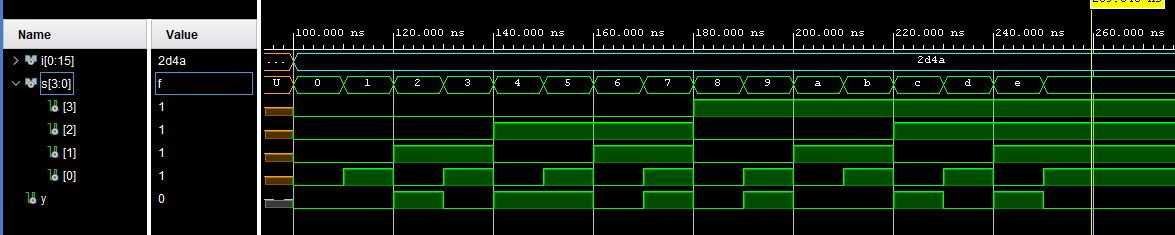
\includegraphics[width=0.95\linewidth]{figure/esercizio1-1/simulazione}
  \caption{Simulazione MUX 16:1}
  \label{fig:esercizio1-1:simulazione}
\end{figure}


\esSezione{Rete di interconnessione 16:4}\label{sec:esercizio1-2}

\begin{traccia}
Utilizzando il componente sviluppato al punto precedente, progettare, implementare in VHDL e testare mediante simulazione una rete di interconnessione a 16 sorgenti e 4 destinazioni.
\end{traccia}

\progetto

La rete comprende due componenti: il multiplexer \texttt{mux\_16\_1}, che seleziona uno dei 16 ingressi mediante il segnale \texttt{s\_i} a 4 bit, e il demultiplexer \texttt{demux\_1\_4}, che ripropone il bit selezionato su una delle 4 uscite in base al segnale \texttt{s\_o} a 2 bit. Il bit intermedio transita nel segnale interno \texttt{q}, di un solo bit. Il multiplexer 16:1 è già stato presentato nell'esercizio~1.1, insieme al multiplexer 4:1 su cui è costruito, ed è qui riutilizzato senza modifiche. La figura~\ref{fig:esercizio1-2:schema} ne riporta lo schema.

\begin{figure}[H]
  \centering
  \begin{tikzpicture}[node distance=2.4cm]
    \node[blocco, minimum height=1.6cm] (mux) {\texttt{mux\_16\_1}};
    \node[blocco, minimum height=1.6cm, right=of mux] (dmux) {\texttt{demux\_1\_4}};
    \draw[bus] ($(mux.west)+(-2.4,0)$) -- node[pos=0.75, sloped, inner sep=1pt]{/} node[pos=0.75, below=3pt, font=\scriptsize]{16} node[pos=0.25, above=3pt, font=\small] {\texttt{x}} (mux.west);
    \draw[seg] (mux.east) -- node[above, font=\small] {\texttt{q}} (dmux.west);
    \draw[bus] (dmux.east) -- node[pos=0.75, sloped, inner sep=1pt]{/} node[pos=0.75, below=3pt, font=\scriptsize]{4} node[pos=0.3, above=3pt, font=\small] {\texttt{y}} ($(dmux.east)+(2.4,0)$);
    \draw[bus] ($(mux.south)+(0,-1.8)$) -- node[pos=0.35, sloped, inner sep=1pt]{/} node[pos=0.35, left=3pt, font=\scriptsize]{4} node[pos=0.35, right=4pt, font=\small] {\texttt{s\_i}} (mux.south);
    \draw[bus] ($(dmux.south)+(0,-1.8)$) -- node[pos=0.35, sloped, inner sep=1pt]{/} node[pos=0.35, left=3pt, font=\scriptsize]{2} node[pos=0.35, right=4pt, font=\small] {\texttt{s\_o}} (dmux.south);
  \end{tikzpicture}
  \caption{Rete di interconnessione 16:4}
  \label{fig:esercizio1-2:schema}
\end{figure}

Il multiplexer riceve il vettore \texttt{x} e la selezione \texttt{s\_i}, mentre il demultiplexer riceve il segnale \texttt{q} e la selezione \texttt{s\_o}: le due selezioni sono indipendenti, per cui ogni ingresso può essere collegato a ogni uscita.

\implementazione

Per il multiplexer 16:1 e per il multiplexer 4:1 si rimanda ai listati~\ref{lst:esercizio1-1:mux-16-1} e~\ref{lst:esercizio1-1:mux-4-1} dell'esercizio~1.1. Rimane da presentare il demultiplexer 1:4.

L'entità \texttt{demux\_1\_4} ha tre porte: l'ingresso \texttt{a} di un bit, la selezione \texttt{s} a 2 bit e l'uscita \texttt{y}, vettore di 4 bit con indici crescenti da 0 a 3. L'architettura è di tipo dataflow: ciascun bit di \texttt{y} è assegnato con un'espressione condizionale \texttt{when ... else}, che porta su di esso il valore di \texttt{a} se \texttt{s} coincide con l'indice del bit e \texttt{'0'} negli altri casi. Le uscite non selezionate restano quindi a zero. Di seguito viene riportato il codice.

\vhdlfile{esercizio1-2/demux_1_4.vhd}{Implementazione DEMUX 1:4}{lst:esercizio1-2:demux-1-4}

Il top module \texttt{interconn16\_4} ha come ingressi il vettore \texttt{x} di 16 bit, la selezione \texttt{s\_i} di 4 bit e la selezione \texttt{s\_o} di 2 bit, e come uscita il vettore \texttt{y} di 4 bit. L'architettura è di tipo structural: il segnale interno \texttt{q}, inizializzato a \texttt{'0'}, collega l'uscita del multiplexer, istanziato con il port mapping \texttt{a => x}, \texttt{s => s\_i}, \texttt{y => q}, all'ingresso \texttt{a} del demultiplexer, il cui port mapping è \texttt{a => q}, \texttt{s => s\_o}, \texttt{y => y}. 

\vhdlfile{esercizio1-2/interconn16_4.vhd}{Implementazione della rete di interconnessione 16:4}{lst:esercizio1-2:interconn16-4}

\simulazione

Il testbench \texttt{interconn16\_4\_tb} ha un'entità senza porte e istanzia il top module con il nome \texttt{INT}. I segnali \texttt{input}, \texttt{ctrl\_in}, \texttt{ctrl\_out} e \texttt{output} sono collegati rispettivamente a \texttt{x}, \texttt{s\_i}, \texttt{s\_o} e \texttt{y}. Il process \texttt{stimuli} verifica il collegamento tra l'ingresso di indice 1 e le quattro uscite: applica a \texttt{input} il valore \texttt{"0101010011000110"}, mantiene per \SI{10}{ns} le selezioni a zero, poi porta \texttt{ctrl\_in} a \texttt{"0001"} e, con un ciclo \texttt{for}, fa variare \texttt{ctrl\_out} da 0 a 3, attendendo \SI{10}{ns} a ogni passo. Al termine di ciascuna attesa un \texttt{assert} controlla che \texttt{output(j)} sia uguale a \texttt{input(1)}, con \texttt{severity failure} in caso contrario; il \texttt{wait} finale sospende il process.

\vhdlfile{esercizio1-2/interconn16_4_tb.vhd}{Testbench rete di interconnessione 16:4}{lst:esercizio1-2:tb}

La simulazione è riportata in figura~\ref{fig:esercizio1-2:simulazione}.

\begin{figure}[H]
  \centering
  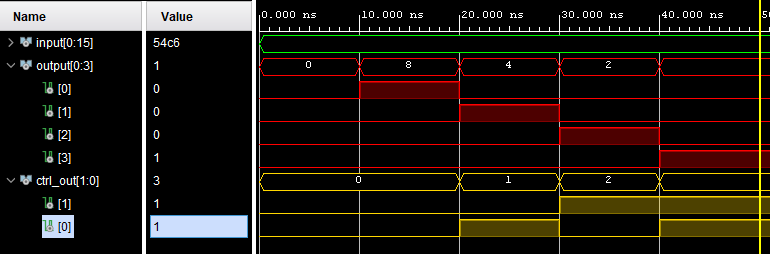
\includegraphics[width=0.9\linewidth]{figure/esercizio1-2/simulazione}
  \caption{Simulazione della rete di interconnessione 16:4}
  \label{fig:esercizio1-2:simulazione}
\end{figure}

L'ingresso \texttt{input[0:15]} vale 0x54C6 ($0101\,0100\,1100\,0110_2$) per tutta la durata mostrata, e il suo bit di indice 1 è \texttt{'1'}. Fino a \SI{10}{ns} le selezioni sono nulle: viene propagato \texttt{input(0)}, pari a \texttt{'0'}, e \texttt{output[0:3]} vale 0x0. A \SI{10}{ns} \texttt{ctrl\_in} diventa $0001_2$, quindi il multiplexer seleziona \texttt{input(1)}. Con \texttt{ctrl\_out} pari a $0_{10}$ l'uscita è 0x8 ($1000_2$), ossia \texttt{output(0)} a \texttt{'1'}; con $1_{10}$ è 0x4 ($0100_2$), con $2_{10}$ è 0x2 ($0010_2$) e con $3_{10}$ è 0x1 ($0001_2$). In ogni intervallo di \SI{10}{ns} è quindi attivo il solo bit selezionato, come richiesto dagli \texttt{assert} del testbench.

\esercizioDaSvolgere{Rete di interconnessione 16:4 su board}{esercizio1-3}


\esCapitolo{Sistema ROM + M}\label{cap:rom-m}
\esSezione{Sistema ROM + M}\label{sec:esercizio2-1}

\begin{traccia}
Progettare, implementare in VHDL e testare mediante simulazione un sistema $S$ composto da una ROM puramente combinatoria di 16 locazioni da 8 bit e da una macchina combinatoria $M$. Fornito un indirizzo $A$ di 4 bit, il sistema restituisce il contenuto della ROM all'indirizzo $A$ trasformato da $M$. Il comportamento di $M$ è a scelta, con il solo vincolo di 8 bit in ingresso e 4 bit in uscita.
\end{traccia}

\progetto

Il sistema è formato da due componenti collegati in cascata: la ROM, che riceve l'indirizzo a 4 bit e fornisce il dato a 8 bit, e la macchina combinatoria $M$, che riduce tale dato a 4 bit. Il sistema è puramente combinatorio, senza clock né reset. Come funzione di $M$ è stata scelta l'AND tra coppie di bit adiacenti del dato letto: ciascuno dei quattro bit di uscita è l'AND di due bit consecutivi dell'ingresso.

Il top module \texttt{systemS} istanzia i due componenti e li collega tramite un segnale interno a 8 bit. Rispetto alla soluzione proposta, l'implementazione usa nomi diversi (\texttt{rom16\_8}, \texttt{systemM}, \texttt{systemS}) e istanzia i componenti in modo diretto (\texttt{entity work.\ldots}) anziché con dichiarazione di \texttt{component}. La struttura del sistema è riassunta in figura~\ref{fig:esercizio2-1:schema}.

\begin{figure}[H]
  \centering
  \begin{tikzpicture}[node distance=2.2cm]
    \node[blocco, minimum width=2.6cm, minimum height=1.4cm] (rom) {\texttt{rom16\_8}\\ (\texttt{MEM})};
    \node[blocco, minimum width=2.6cm, minimum height=1.4cm, right=of rom] (m) {\texttt{systemM}\\ (\texttt{SYSTEM\_M})};
    \node[draw, dashed, thick, inner xsep=0.6cm, inner ysep=0.5cm, fit=(rom)(m), label={[font=\sffamily\small]above:\texttt{systemS}}] (s) {};
    \draw[bus] ($(s.west |- rom)+(-2.4,0)$) -- node[pos=0.2, above=3pt, font=\scriptsize] {\texttt{input}} node[pos=0.5, sloped, inner sep=1pt]{/} node[pos=0.5, below=3pt, font=\scriptsize]{4} (rom.west);
    \draw[bus] (rom) -- node[pos=0.5, sloped, inner sep=1pt]{/} node[pos=0.5, below=3pt, font=\scriptsize]{8} node[pos=0.5, above=3pt, font=\scriptsize] {\texttt{q}} (m);
    \draw[bus] (m.east) -- node[pos=0.5, sloped, inner sep=1pt]{/} node[pos=0.5, below=3pt, font=\scriptsize]{4} node[pos=0.88, above=3pt, font=\scriptsize] {\texttt{output}} ($(s.east |- m)+(2.4,0)$);
  \end{tikzpicture}
  \caption{Schema a blocchi del sistema ROM + M}
  \label{fig:esercizio2-1:schema}
\end{figure}

\implementazione

L'entità \texttt{rom16\_8} ha come ingresso \texttt{address} (4 bit) e come uscita \texttt{data} (8 bit). Nell'architettura \texttt{Behavioral} si trova un array di 16 elementi da 8 bit, inizializzato con valori esadecimali, e un process, sensibile ad \texttt{address}, assegna a \texttt{data} l'elemento indicato dall'indirizzo convertito in intero. L'attributo \texttt{rom\_style} è impostato a \texttt{"block"}. Il contenuto della ROM (da 0x4A a 0xED) differisce da quello della soluzione proposta (0xA8, 0xBD, \ldots), che ripete due volte la stessa serie di otto valori.

\vhdlfile{esercizio2-1/rom16_8.vhd}{Implementazione ROM 16x8}{lst:esercizio2-1:rom16-8}

L'entità \texttt{systemM} ha l'ingresso \texttt{data\_in} (8 bit) e l'uscita \texttt{data\_out} (4 bit). L'architettura \texttt{dataflow} assegna a ciascun bit di uscita l'AND di due bit adiacenti: \texttt{data\_out(0)} da \texttt{data\_in(0)} e \texttt{data\_in(1)}, \texttt{data\_out(1)} da \texttt{data\_in(2)} e \texttt{data\_in(3)}, e così via fino a \texttt{data\_out(3)}. A differenza della soluzione proposta, le porte sono dichiarate con indici decrescenti (\texttt{7 downto 0}).

\vhdlfile{esercizio2-1/systemm.vhd}{Implementazione macchina combinatoria M}{lst:esercizio2-1:systemm}

Definite le due entità, il top module \texttt{systemS} ha l'ingresso \texttt{input} e l'uscita \texttt{output}, entrambi a 4 bit. L'architettura \texttt{structural} dichiara il segnale \texttt{q}, a 8 bit, che porta il dato dalla ROM a $M$, e istanzia \texttt{rom16\_8} (etichetta \texttt{MEM}) e \texttt{systemM} (etichetta \texttt{SYSTEM\_M}) con port mapping per nome.

\vhdlfile{esercizio2-1/systems.vhd}{Implementazione del sistema ROM + M}{lst:esercizio2-1:systems}

\simulazione

Il testbench \texttt{systemS\_tb} ha entità senza porte. Istanzia il sistema sotto test (\texttt{SYSTEM\_S}) e una seconda istanza di \texttt{systemM}, usata come riferimento, alimentata con i valori di una copia della ROM (\texttt{ref\_mem}) dichiarata nel testbench. Il process \texttt{stim\_proc} attende \SI{10}{ns}, poi con un ciclo \texttt{for} da 0 a 15 applica l'indirizzo \texttt{x} e carica in \texttt{ref\_in} il dato corrispondente. Dopo \SI{10}{ns} confronta \texttt{y} con \texttt{ref\_out} tramite \texttt{assert}, con \texttt{severity failure} in caso di differenza, e termina con \texttt{wait;}.

\vhdlfile{esercizio2-1/systems_tb.vhd}{Testbench sistema ROM + M}{lst:esercizio2-1:systems-tb}

Il risultato della simulazione è mostrato in figura~\ref{fig:esercizio2-1:simulazione}.

\begin{figure}[H]
  \centering
  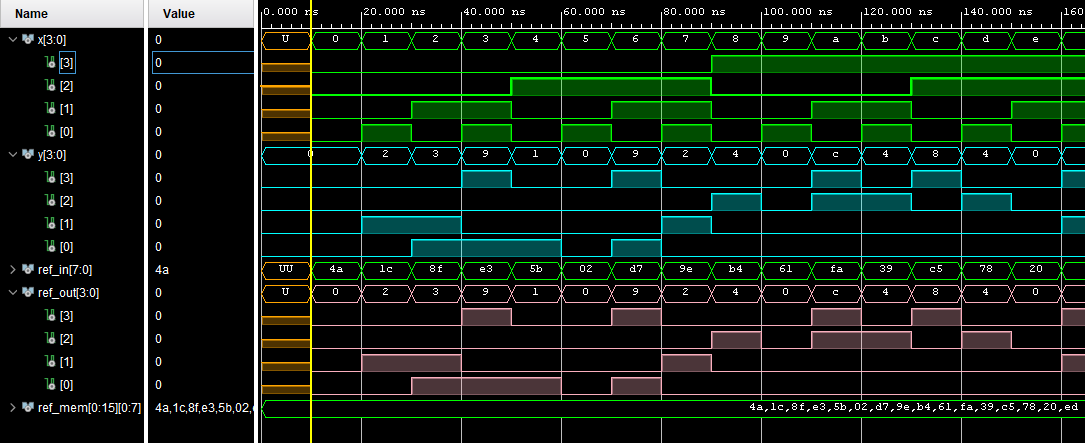
\includegraphics[width=0.95\linewidth]{figure/esercizio2-1/simulazione}
  \caption{Simulazione sistema ROM + M}
  \label{fig:esercizio2-1:simulazione}
\end{figure}

Per l'indirizzo \texttt{x} $= 1$ ($0001_2$) il sistema legge dalla ROM il valore 0x1C ($00011100_2$), presente in \texttt{ref\_in}. Le coppie di bit adiacenti, dalla meno significativa, valgono $00$, $11$, $01$, $00$: l'uscita \texttt{y} è quindi $0010_2$, cioè 2 in esadecimale, uguale a \texttt{ref\_out}. Lo stesso vale per tutti i sedici indirizzi e l'\texttt{assert} non segnala errori.

\begin{risultato}
Per i sedici indirizzi, \texttt{y} coincide con \texttt{ref\_out} (ad esempio 0x2 per l'indirizzo 1 e 0x3 per l'indirizzo 2).
\end{risultato}

\esSezione{Sistema ROM + M su board}\label{sec:esercizio2-2}

\begin{traccia}
Sintetizzare ed implementare su board il progetto del sistema ROM+M sviluppato al punto 2.1, utilizzando gli switch per fornire l'indirizzo della ROM da cui leggere i valori da trasformare e i led per visualizzare i 4 bit di uscita.
\end{traccia}

\progetto

Il sistema $S$ è già stato progettato e descritto nell'esercizio~\ref{sec:esercizio2-1}: non viene modificato. Per portarlo su board si aggiunge un solo componente, un top module che espone le porte fisiche della scheda e le collega a quelle di \texttt{systemS}. Il sistema è puramente combinatorio, quindi usiamo solo switch e led.

\implementazione

I componenti \texttt{rom16\_8}, \texttt{systemM} e \texttt{systemS} sono quelli presentati nell'esercizio~\ref{sec:esercizio2-1} (listati~\ref{lst:esercizio2-1:rom16-8}, \ref{lst:esercizio2-1:systemm} e~\ref{lst:esercizio2-1:systems}) e non vengono ivi riportati.

L'entità \texttt{systemS\_tl} ha l'ingresso \texttt{SW} e l'uscita \texttt{LED}, entrambi a 4 bit. L'architettura \texttt{structural} non dichiara segnali interni e contiene una sola istanza di \texttt{systemS}, con etichetta \texttt{SYSTEM\_S}, il cui port mapping per nome collega \texttt{input} a \texttt{SW} e \texttt{output} a \texttt{LED}. 

\vhdlfile{esercizio2-2/systems_tl.vhd}{Implementazione del top module su board}{lst:esercizio2-2:systems-tl}

\sintesiboard

Gli interruttori \texttt{SW[0]}--\texttt{SW[3]} della scheda Nexys A7-100T forniscono l'indirizzo $A$ della ROM, mentre i LED \texttt{LED[0]}--\texttt{LED[3]} mostrano il valore a 4 bit prodotto da $M$. Cambiando la configurazione degli interruttori si ottiene sui LED il risultato dell'AND tra coppie di bit adiacenti del contenuto della locazione selezionata.

% TODO: foto della scheda e verifica del comportamento su board, non disponibili nel progetto

Nel file dei constraint sono state decommentate le seguenti righe, che assegnano ai quattro interruttori e ai quattro LED i rispettivi pin della scheda, con standard di I/O \texttt{LVCMOS33}.

\xdcfile{esercizio2-2/vincoli.xdc}{Constraint}{lst:esercizio2-2:vincoli}

\begin{figure}[H]
  \centering
  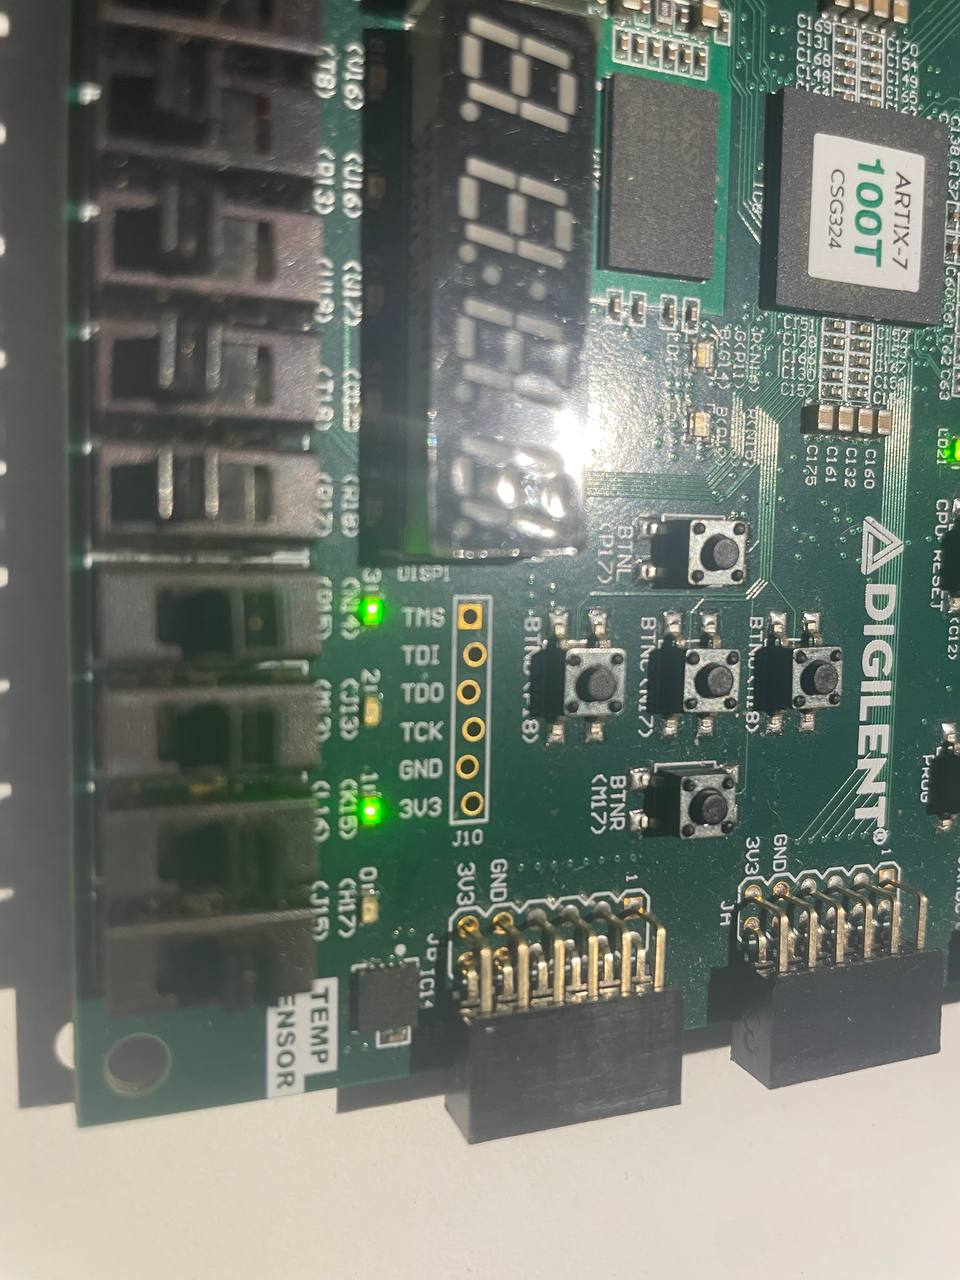
\includegraphics[width=0.7\linewidth]{figure/esercizio2-2/irl.jpg}
  \caption{Realizzazione sistema ROM + M}
  \label{fig:esercizio2-2:realizzazione}
\end{figure}


\esCapitolo{Riconoscitore di sequenza}\label{cap:riconoscitore-sequenza}
\esSezione{Riconoscitore della sequenza 101}\label{sec:esercizio3-1}

\begin{traccia}
Progettare, implementare in VHDL e testare mediante simulazione una macchina che riconosce la sequenza \texttt{101}. La macchina riceve un dato binario seriale $i$, un segnale di tempificazione $A$ e un segnale di modo $M$, e porta a '1' l'uscita $Y$ quando la sequenza viene riconosciuta. Se $M=0$ i bit sono valutati a gruppi di tre, senza sovrapposizione; se $M=1$ i bit sono valutati uno alla volta e la macchina torna allo stato iniziale a ogni riconoscimento (sequenze parzialmente sovrapposte).
\end{traccia}

\progetto

Il riconoscitore è una macchina a stati finiti di tipo Mealy, dal momento che l'uscita \texttt{y} dipende sia dallo stato corrente sia dall'ingresso \texttt{i}. È descritta con due process: uno combinatorio per la funzione di stato prossimo e di uscita, uno sincrono per il registro di stato. Il segnale di tempificazione \texttt{a} svolge il ruolo di clock della macchina e il reset \texttt{rst} è sincrono rispetto ad esso.

Gli stati sono sette, divisi in due sottografi, uno per modo, con lo stato iniziale \texttt{S0} in comune:
\begin{enumerate}
  \item modo 1 (un bit alla volta): \texttt{S0} (nessun bit utile), \texttt{S1} (visto '1'), \texttt{S2} (visto "10");
  \item modo 0 (gruppi di tre bit): \texttt{G1} (primo bit del gruppo pari a '1'), \texttt{G1E} (primo bit sbagliato), \texttt{G2} (letto "10"), \texttt{G2E} (gruppo ormai perso).
\end{enumerate}
In modo 0 gli stati terminano sempre dopo tre bit, con ritorno in \texttt{S0}, così da preparare il gruppo successivo. In modo 1, dopo il riconoscimento la macchina torna in \texttt{S0}; un '1' immediatamente successivo è quindi trattato come inizio di una nuova sequenza solo dal bit seguente, mentre l'autoanello su \texttt{S1} gestisce i '1' consecutivi. Il diagramma è riportato in figura~\ref{fig:esercizio3-1:stati}, con etichette nel formato \texttt{M i / Y}.

\begin{figure}[H]
  \centering
  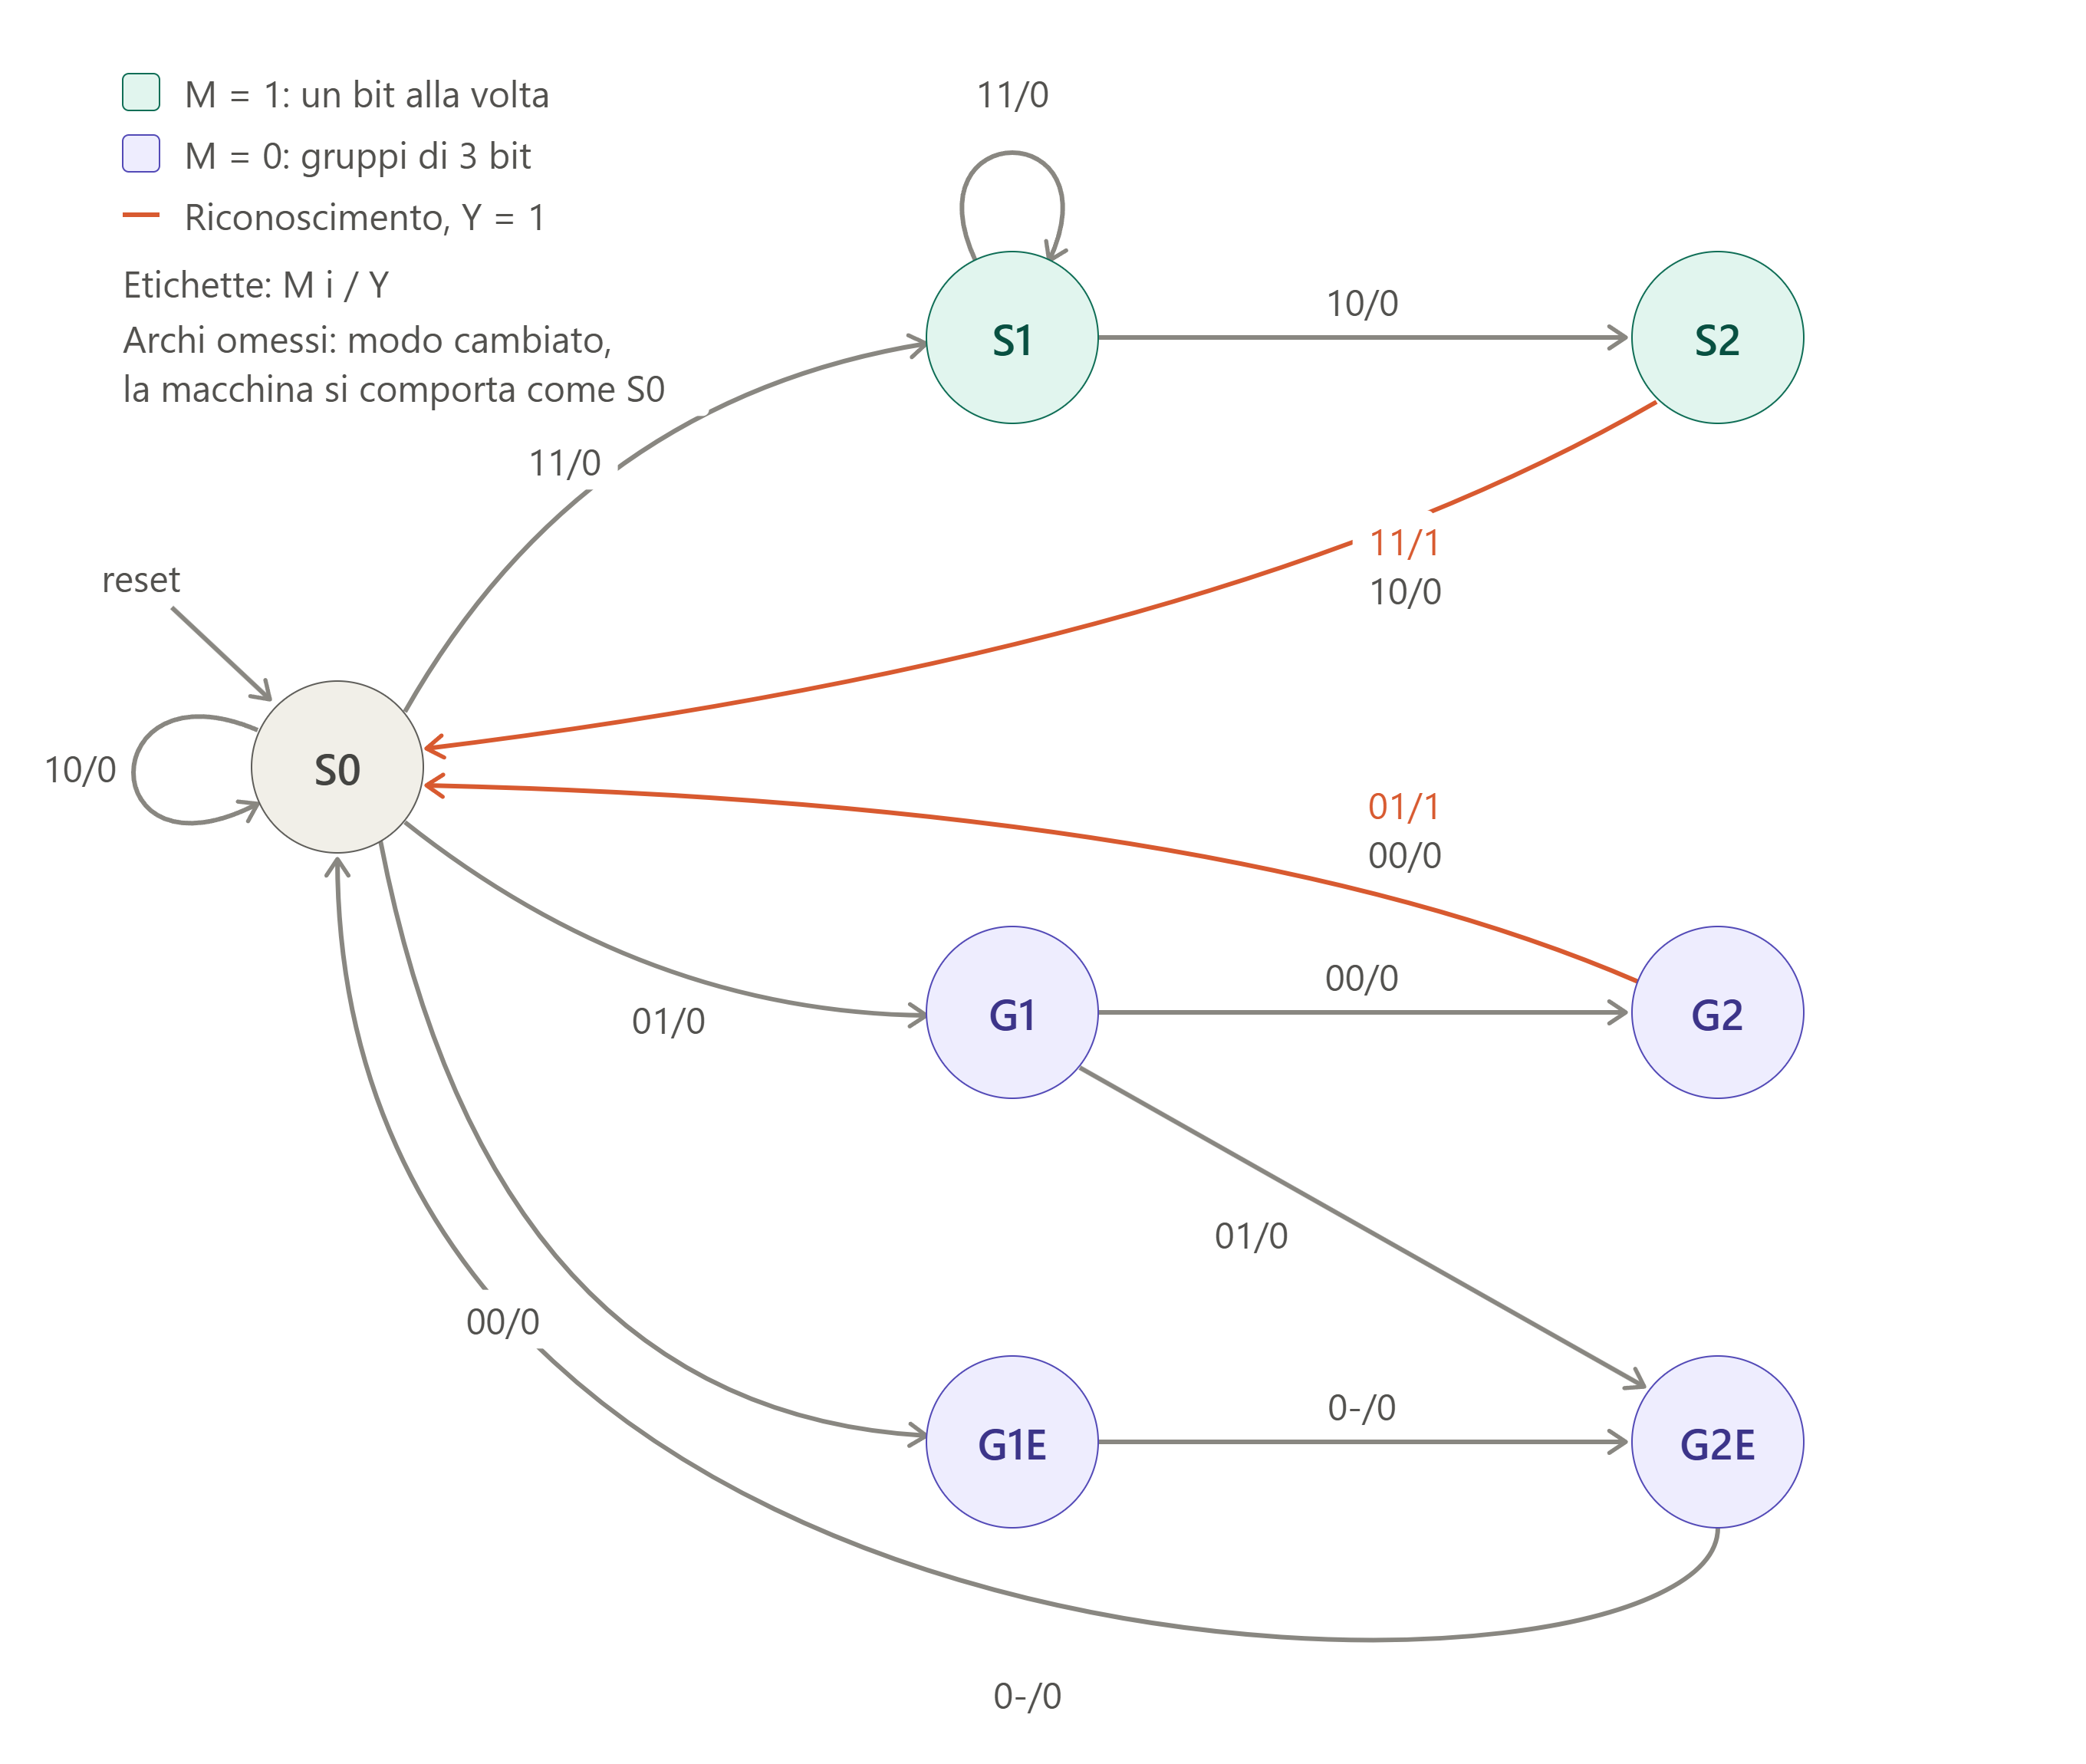
\includegraphics[width=0.75\linewidth]{figure/esercizio3-1/stati}
  \caption{FSM del riconoscitore 101}
  \label{fig:esercizio3-1:stati}
\end{figure}

Gli stati verdi appartengono al modo 1 e quelli viola al modo 0; l'arco arancione indica le transizioni con uscita a '1'. Gli archi nei quali il modo risulta cambiato rispetto allo stato in cui ci si trova sono omessi: in tal caso la macchina si comporta come se fosse in \texttt{S0} del nuovo modo, senza perdere il bit in ingresso.

\implementazione

L'entità \texttt{fsm\_sequence} ha cinque porte di tipo \texttt{std\_logic}: gli ingressi \texttt{i} (dato), \texttt{m} (modo), \texttt{a} (tempificazione) e \texttt{rst} (reset), e l'uscita \texttt{y}. L'architettura \texttt{Behavioral} definisce il tipo enumerato \texttt{state} con i sette stati e i segnali \texttt{current\_state} e \texttt{next\_state}.

Il process \texttt{f\_stato\_uscita} ha come sensitivity list \texttt{current\_state}, \texttt{m} e \texttt{i}. In testa assegna i valori di default: \texttt{y} a '0' e lo stato prossimo ottenuto come se la macchina fosse in \texttt{S0} per il modo corrente. Il costrutto \texttt{case} sullo stato corrente sovrascrive poi solo le transizioni diverse dal default, e ciascuna di esse è condizionata al modo coerente con lo stato: se \texttt{m} non lo è, resta valido il default e la macchina riparte come da \texttt{S0}. Il process \texttt{mem} è sensibile ad \texttt{a}: sul fronte di salita carica \texttt{S0} se \texttt{rst} vale '1', altrimenti \texttt{next\_state}.

\vhdlfile{esercizio3-1/fsm_sequence.vhd}{Implementazione del riconoscitore di sequenza}{lst:esercizio3-1:fsm}

\simulazione

Il testbench \texttt{fsm\_sequence\_tb} ha un'entità senza porte e istanzia il componente da verificare come \texttt{dut}. Il process \texttt{clk\_proc} genera il segnale \texttt{A} con periodo di \SI{10}{\nano\second} (costante \texttt{T}); il process \texttt{stim} applica gli ingressi, cambiando \texttt{i} a ogni periodo e riportando la macchina in reset tra un test e il successivo. Termina con un \texttt{wait} senza condizione. I test sono quattro:
\begin{enumerate}
  \item $M=1$, ingresso \texttt{010101}: la sequenza è riconosciuta al quarto bit; l'ultimo '1' non produce uscita;
  \item $M=0$, ingresso \texttt{010101}: il primo gruppo \texttt{010} non è valido, il secondo \texttt{101} è riconosciuto al sesto bit;
  \item $M=1$, ingresso \texttt{1101}: il riconoscimento avviene al quarto bit grazie all'autoanello su \texttt{S1};
  \item cambio di modo a metà sequenza: con $M=0$ si leggono \texttt{1} e \texttt{0}, poi $M$ passa a '1' e si leggono \texttt{1}, \texttt{0}, \texttt{1}; la macchina riparte da \texttt{S0} e riconosce la sequenza all'ultimo bit.
\end{enumerate}

\vhdlfile{esercizio3-1/fsm_sequence_tb.vhd}{Testbench del riconoscitore di sequenza}{lst:esercizio3-1:tb}

Il risultato della simulazione è mostrato in figura~\ref{fig:esercizio3-1:simulazione}.

\begin{figure}[H]
  \centering
  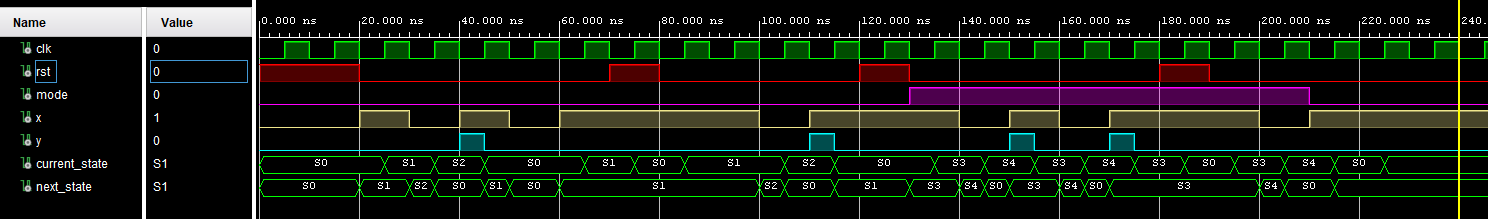
\includegraphics[width=\linewidth]{figure/esercizio3-1/simulazione}
  \caption{Simulazione del riconoscitore 101}
  \label{fig:esercizio3-1:simulazione}
\end{figure}

Consideriamo il primo test. Terminato il reset a \SI{20}{\nano\second}, con $M=1$ vengono applicati i bit \texttt{0}, \texttt{1}, \texttt{0}, \texttt{1}, uno per periodo di \texttt{A}: lo stato corrente passa da \texttt{S0} a \texttt{S1}, poi a \texttt{S2}. Quando il quarto bit, pari a '1', è presente in ingresso (intorno a \SI{50}{\nano\second}) la macchina è in \texttt{S2} e \texttt{Y} sale a '1'; al fronte di \texttt{A} successivo lo stato torna a \texttt{S0} e \texttt{Y} ridiventa '0'. Poiché \texttt{Y} dipende anche da \texttt{i}, l'uscita è un impulso della durata di mezzo periodo di \texttt{A}. Gli stessi impulsi si ritrovano nei tre test successivi, in corrispondenza dell'ultimo bit della sequenza riconosciuta.

\begin{risultato}
In tutti e quattro i test l'uscita \texttt{Y} assume il valore '1' una sola volta, in corrispondenza dell'ultimo bit della sequenza \texttt{101}.
\end{risultato}

\esercizioDaSvolgere{Riconoscitore di sequenza su board}{esercizio3-2}


\esCapitolo{Shift register}\label{cap:shift-register}
\esSezione{Shift register}\label{sec:esercizio4-1}

\begin{traccia}
Progettare, implementare in VHDL e testare mediante simulazione un registro a scorrimento di N bit in grado di shiftare a destra o a sinistra di un numero Y variabile di posizioni a seconda di una opportuna selezione. In particolare, i valori possibili di Y sono 1 e 2. L'utente tramite selezione deve scegliere di quante posizioni shiftare. Il componente deve essere realizzato utilizzando sia un a) approccio comportamentale sia un b) approccio strutturale. Nota: il numero di bit del registro deve essere implementato come un generic, e dall'esterno deve poter essere scelta la modalità di funzionamento mediante opportuni segnali di selezione.
\end{traccia}

\progetto

Il registro è descritto da un'unica entità, \texttt{shift\_register}, dotata di due architetture: \texttt{Behavioral} e \texttt{structural}. Le due condividono la stessa interfaccia, per poterle istanziare entrambe nel testbench e confrontarne le uscite. Il generic \texttt{N} fissa la larghezza; gli ingressi \texttt{dir} e \texttt{pos} selezionano rispettivamente il verso (\texttt{'0'} destra, \texttt{'1'} sinistra) e il numero di posizioni (\texttt{'0'} una, \texttt{'1'} due), mentre \texttt{en} abilita lo scorrimento e \texttt{load} il caricamento parallelo del dato \texttt{d}. Il reset \texttt{rst} è sincrono e ha la precedenza su \texttt{load}, che a sua volta ha la precedenza su \texttt{en}. Nello scorrimento i bit che entrano valgono \texttt{'0'}.

\subsection*{}
\esSottosezione{Approccio comportamentale}

\implementazione

L'architettura \texttt{Behavioral} contiene un solo process con sensitivity list limitata a \texttt{clk}, attivo sul fronte di salita. Il registro interno \texttt{r} viene azzerato se \texttt{rst} vale \texttt{'1'}, altrimenti caricato con \texttt{d} se \texttt{load} vale \texttt{'1'}; se invece è attivo \texttt{en}, viene aggiornato con una concatenazione che dipende da \texttt{dir} e \texttt{pos}, ad esempio \texttt{'0' \& r(N-1 downto 1)} per lo scorrimento a destra di una posizione. Se nessun controllo è attivo il valore si mantiene. Un'istruzione \texttt{assert} controlla in fase di elaborazione che \texttt{N} sia almeno 2; l'uscita \texttt{q} è assegnata in modo concorrente a \texttt{r}. Si riportano di seguito l'entità e la prima architettura.

\vhdlfile[firstline=1,lastline=52]{esercizio4-1/shift_register.vhd}{Implementazione comportamentale dello shift register}{lst:esercizio4-1:shift-register-beh}

\esSottosezione{Approccio strutturale}

\progetto

La versione strutturale replica per ogni bit una slice, illustrata nella figura~\ref{fig:esercizio4-1:rtl}. Il flip-flop D è preceduto da due multiplexer 2:1 in cascata e da un multiplexer 4:1. Il multiplexer 4:1 sceglie il nuovo valore del bit tra i quattro bit adiacenti (a distanza 1 e 2, a destra e a sinistra) in base a \texttt{dir} e \texttt{pos}; il primo multiplexer 2:1 sceglie tra questo valore e il dato \texttt{d(i)} in base a \texttt{load}; il secondo mantiene il valore corrente \texttt{r(i)} quando né \texttt{load} né \texttt{en} sono attivi, ed è comandato dal segnale \texttt{we}, ottenuto come \texttt{load or en}. 
\begin{figure}[H]
  \centering
  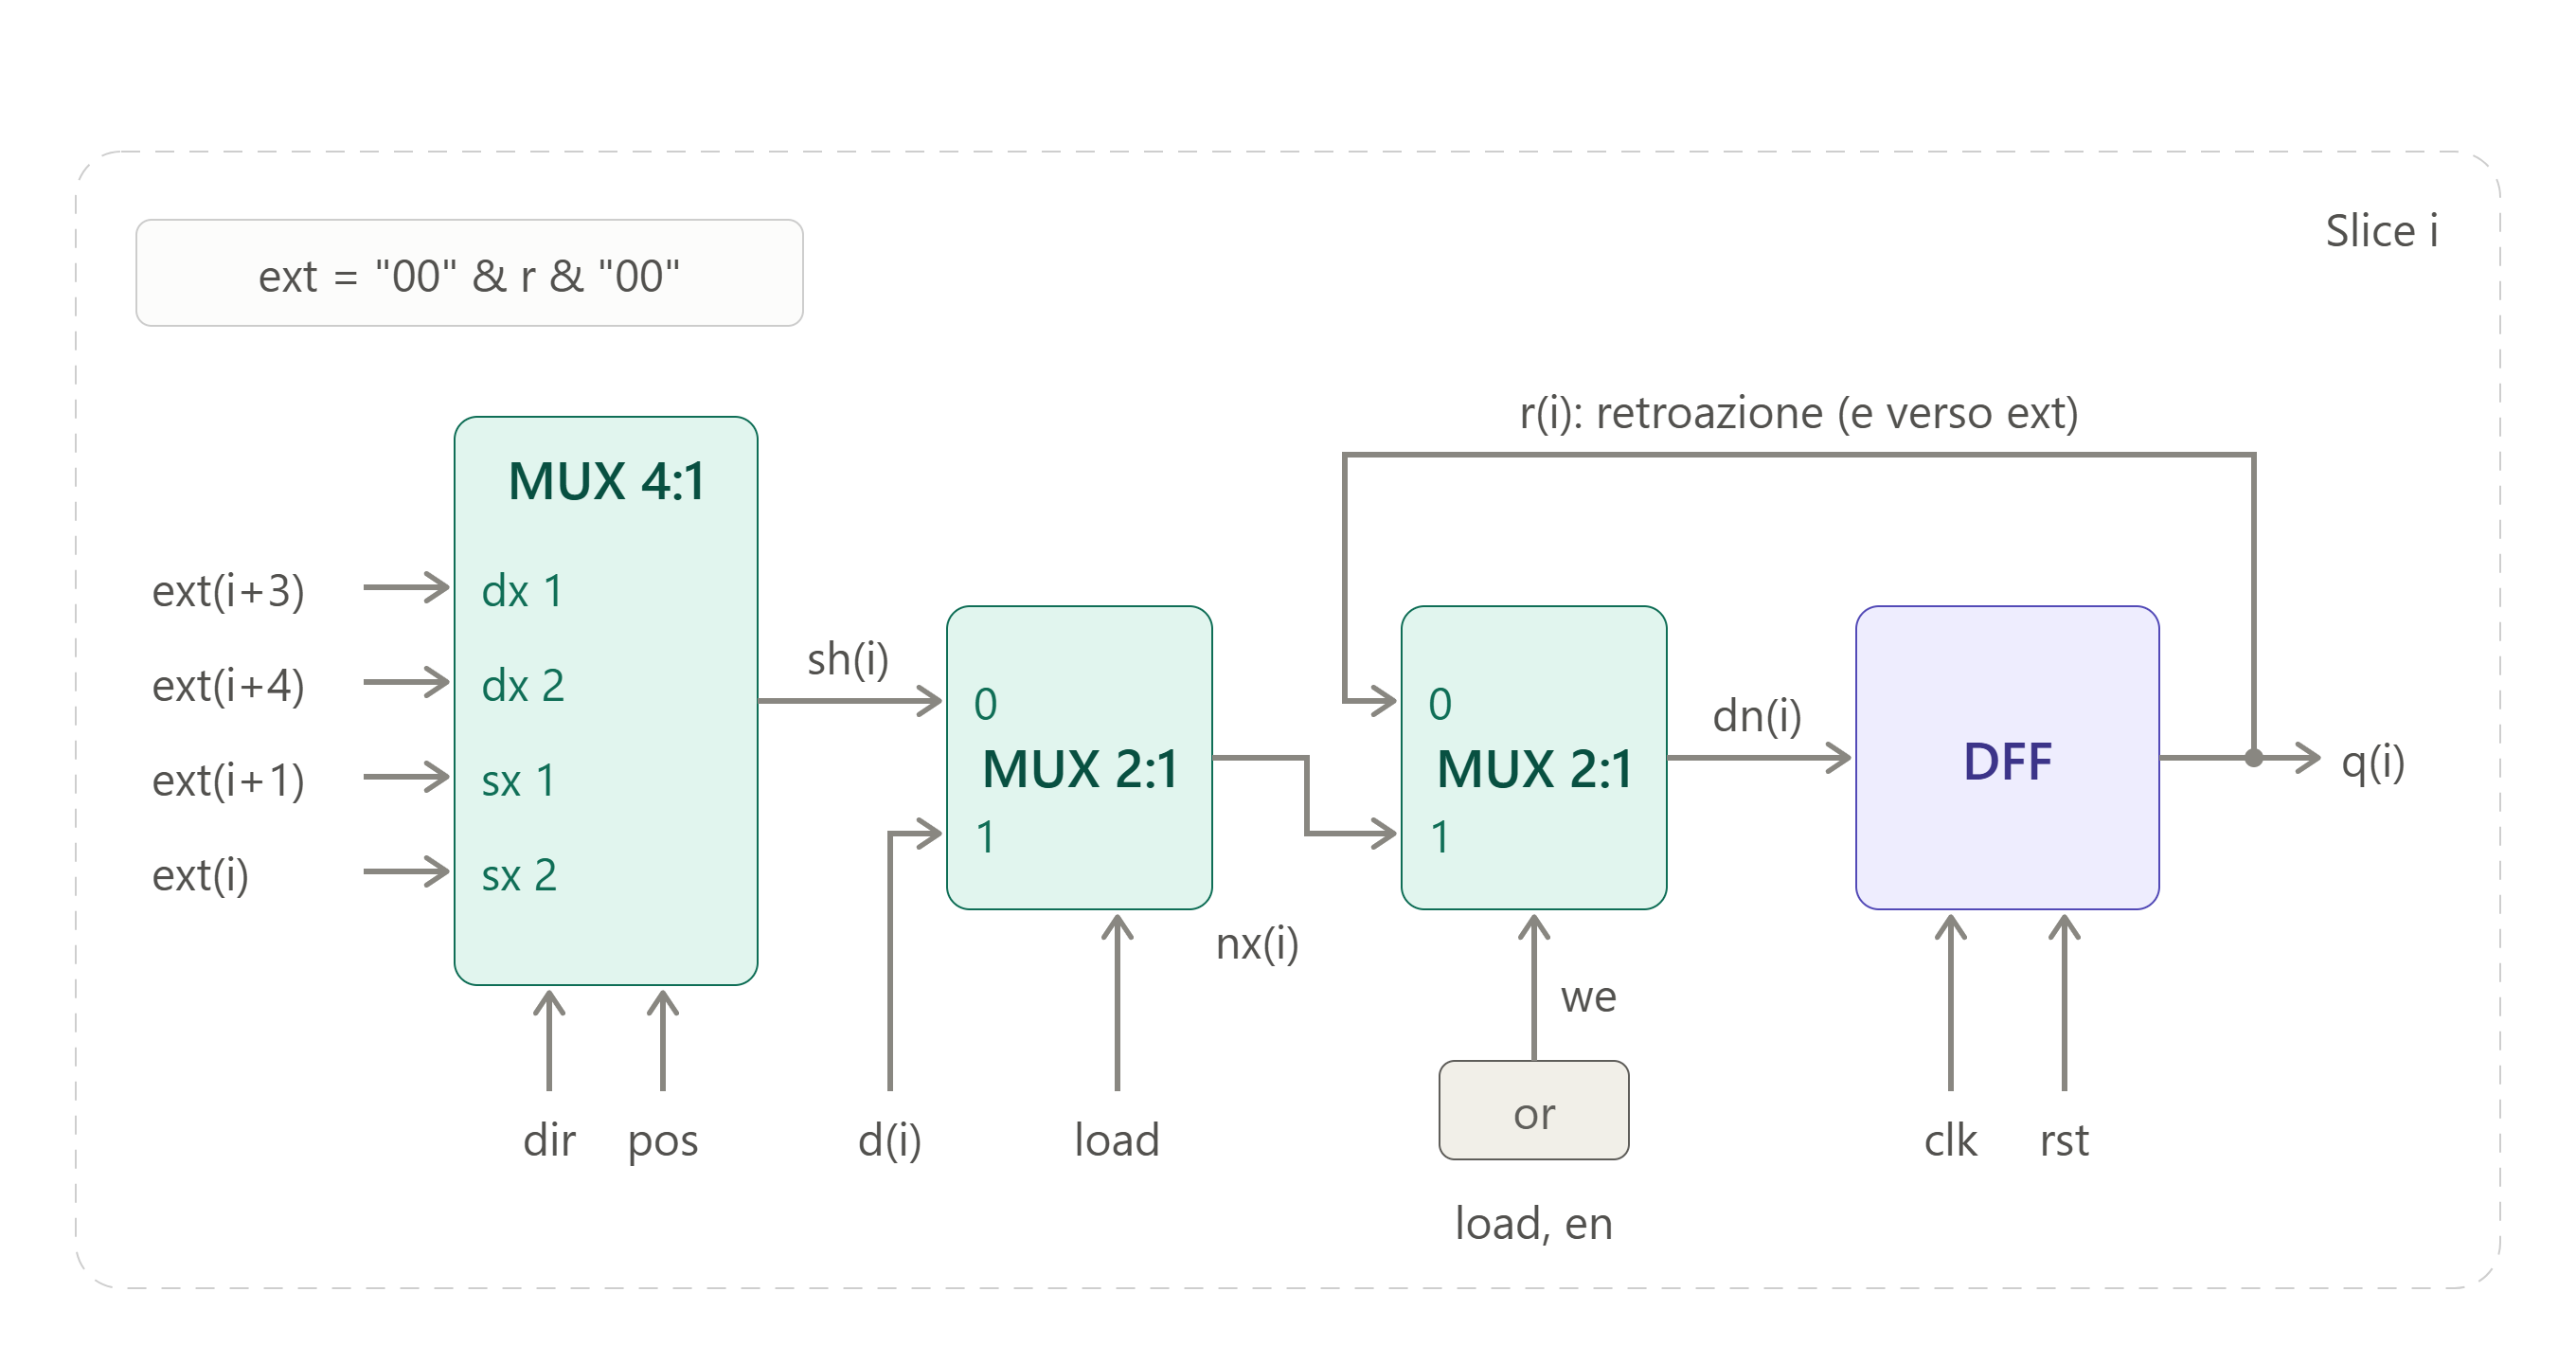
\includegraphics[width=0.75\linewidth]{figure/esercizio4-1/rtl}
  \caption{Slice i-esima dello shift register strutturale}
  \label{fig:esercizio4-1:rtl}
\end{figure}

Per gestire i bit di bordo, il segnale \texttt{ext}, di $N+4$ bit, è ottenuto affiancando due zeri a ciascun estremo di \texttt{r}; in questo modo \texttt{ext(i+3)} e \texttt{ext(i+4)} corrispondono a \texttt{r(i+1)} e \texttt{r(i+2)}, mentre \texttt{ext(i+1)} ed \texttt{ext(i)} corrispondono a \texttt{r(i-1)} e \texttt{r(i-2)}, e i bit fuori dal registro valgono \texttt{'0'}.

\implementazione

Il flip-flop D è l'entità \texttt{dff}, con ingressi \texttt{clk}, \texttt{rst} e \texttt{d} e uscita \texttt{q}, tutti a un bit. L'architettura \texttt{behavioral} è un process sul fronte di salita del clock, con reset sincrono che porta l'uscita a \texttt{'0'}.

\vhdlfile{esercizio4-1/dff.vhd}{Implementazione flip-flop D}{lst:esercizio4-1:dff}

Il multiplexer 2:1 è l'entità \texttt{mux\_2\_1}, con ingressi \texttt{a0} e \texttt{a1}, selezione \texttt{s} e uscita \texttt{y} (usiamo la semplice architettura \texttt{dataflow}).

\vhdlfile{esercizio4-1/mux_2_1.vhd}{Implementazione MUX 2:1}{lst:esercizio4-1:mux-2-1}

Il multiplexer 4:1 è già stato presentato nel listato~\ref{lst:esercizio1-1:mux-4-1} dell'esercizio~1.1; qui si usa l'architettura \texttt{dataflow}.

L'architettura \texttt{structural} dichiara i segnali \texttt{r} (uscite dei flip-flop), \texttt{ext}, \texttt{sh} (uscite dei multiplexer 4:1), \texttt{nx} (valore scelto tra scorrimento e caricamento), \texttt{dn} (ingresso dei flip-flop) e \texttt{we}. Un ciclo \texttt{for generate} istanzia, per ciascun indice \texttt{i}, i componenti \texttt{m\_shift}, \texttt{m\_load}, \texttt{m\_hold} e \texttt{ff} con port mapping. Nel multiplexer 4:1 la selezione è composta da \texttt{dir} (bit più significativo) e \texttt{pos} (bit meno significativo), per cui i valori \texttt{"00"}, \texttt{"01"}, \texttt{"10"} e \texttt{"11"} corrispondono a scorrimento a destra di 1, a destra di 2, a sinistra di 1 e a sinistra di 2. Il reset è collegato ai flip-flop, mentre l'uscita \texttt{q} è assegnata a \texttt{r}. Il codice è il seguente.

\vhdlfile[firstline=54,lastline=95]{esercizio4-1/shift_register.vhd}{Implementazione strutturale dello shift register}{lst:esercizio4-1:shift-register-str}

\simulazione

Il testbench \texttt{shift\_register\_tb} ha entità senza porte e fissa \texttt{N} a 8 e il periodo del clock a \SI{10}{ns}. Sono istanziate due copie del componente, \texttt{dut\_beh} con architettura \texttt{Behavioral} e \texttt{dut\_str} con architettura \texttt{structural}, collegate agli stessi ingressi e con uscite distinte \texttt{q\_beh} e \texttt{q\_str}. Il process \texttt{clk\_proc} genera il clock; il process \texttt{stim} applica gli stimoli; il process \texttt{check} confronta le due uscite a ogni fronte di discesa e segnala con \texttt{assert} l'eventuale divergenza. I passi di prova sono i seguenti.

\begin{enumerate}
  \item Reset per due periodi, con \texttt{rst} a \texttt{'1'}.
  \item Caricamento parallelo di \texttt{"10110011"} (0xB3).
  \item Con \texttt{en} a \texttt{'1'}, quattro scorrimenti consecutivi: destra di 1, destra di 2, sinistra di 1, sinistra di 2.
  \item Mantenimento del valore con \texttt{en} a \texttt{'0'} per due periodi.
  \item Attivazione simultanea di \texttt{load} ed \texttt{en} con \texttt{d} pari a \texttt{"11110000"} (0xF0): prevale il caricamento.
  \item Attivazione simultanea di \texttt{rst} e \texttt{load}: prevale il reset.
\end{enumerate}

\vhdlfile{esercizio4-1/shift_register_tb.vhd}{Testbench dello shift register}{lst:esercizio4-1:tb}

Il risultato della simulazione è mostrato in figura~\ref{fig:esercizio4-1:simulazione}, dove sono visibili anche i singoli bit di \texttt{q\_str}.

\begin{figure}[H]
  \centering
  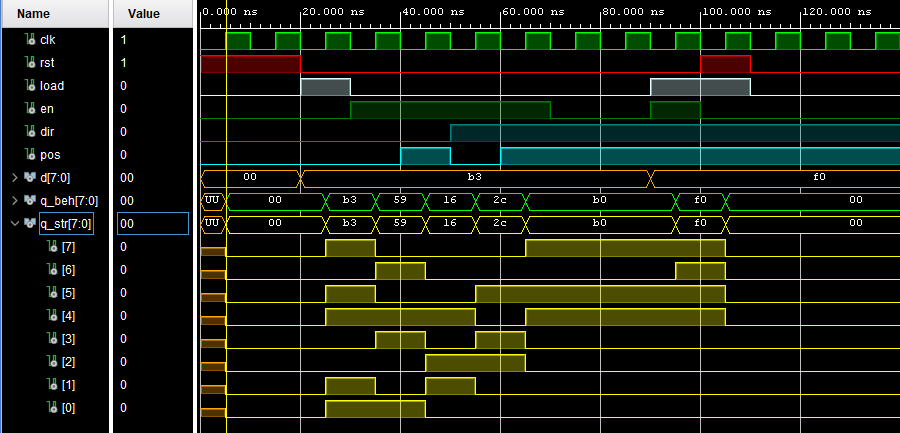
\includegraphics[width=0.95\linewidth]{figure/esercizio4-1/simulazione}
  \caption{Simulazione dello shift register}
  \label{fig:esercizio4-1:simulazione}
\end{figure}

Dopo il reset, con \texttt{load} a \texttt{'1'} e \texttt{d} pari a 0xB3 ($1011\,0011_2$), le due uscite \texttt{q\_beh} e \texttt{q\_str} assumono il valore b3 al fronte di clock successivo. Con \texttt{en} attivo e \texttt{dir} e \texttt{pos} a \texttt{'0'}, il valore diventa 0x59 ($0101\,1001_2$), ossia lo scorrimento a destra di una posizione; con \texttt{pos} a \texttt{'1'} diventa 0x16 ($0001\,0110_2$), a destra di due; con \texttt{dir} a \texttt{'1'} e \texttt{pos} a \texttt{'0'} diventa 0x2C ($0010\,1100_2$), a sinistra di una; infine con \texttt{pos} a \texttt{'1'} diventa 0xB0 ($1011\,0000_2$), a sinistra di due. Il valore 0xB0 resta invariato mentre \texttt{en} è a \texttt{'0'}. Al caricamento simultaneo con \texttt{en} le uscite passano a 0xF0, e all'ultimo impulso di \texttt{rst}, applicato insieme a \texttt{load}, tornano a 0x00. In tutti i passi le due uscite coincidono.

\begin{risultato}
Le uscite \texttt{q\_beh} e \texttt{q\_str} coincidono lungo tutta la simulazione: b3, 59, 16, 2c, b0, f0 e infine 00.
\end{risultato}


\esCapitolo{Cronometro}\label{cap:cronometro}
\esSezione{Cronometro}\label{sec:esercizio5-1}

\begin{traccia}
Progettare, implementare in VHDL e testare mediante simulazione un cronometro, in grado di scandire secondi, minuti e ore a partire da una base dei tempi prefissata (es.\ si consideri il clock a disposizione sulla board). Il progetto deve prevedere la possibilità di inizializzare il cronometro con un valore iniziale, sempre espresso in termini di ore, minuti e secondi, mediante un opportuno ingresso di set, e deve prevedere un ingresso di reset per azzerare il tempo. Il componente deve essere realizzato utilizzando un approccio strutturale, collegando opportunamente dei contatori secondo uno schema a scelta.
\end{traccia}

\progetto

Il cronometro è ottenuto dalla cascata di quattro istanze dello stesso componente, il contatore modulare \texttt{counter\_mod}, che verrà riutilizzato anche negli esercizi successivi. La prima istanza, il prescaler, ha modulo \texttt{F\_CLK}, pari al numero di cicli di clock contenuti in un secondo, e produce un impulso \texttt{tick} una volta al secondo. Fa quindi da divisore di frequenza. Il conteggio dei secondi è comunque pilotato da un segnale di abilitazione, così tutto il circuito resta sincrono con il clock della board.

Le tre istanze successive contano i secondi (modulo 60, 6 bit), i minuti (modulo 60, 6 bit) e le ore (modulo 24, 5 bit). L'uscita di riporto \texttt{tc} di ciascun contatore abilita quello successivo: \texttt{tick} abilita i secondi, \texttt{tc\_s} i minuti e \texttt{tc\_m} le ore. Clock, reset e set sono comuni a tutti i contatori, mentre \texttt{run} abilita il solo prescaler e permette di fermare il conteggio. Lo schema è visibile in figura~\ref{fig:esercizio5-1:schema}.

\begin{figure}[H]
  \centering
  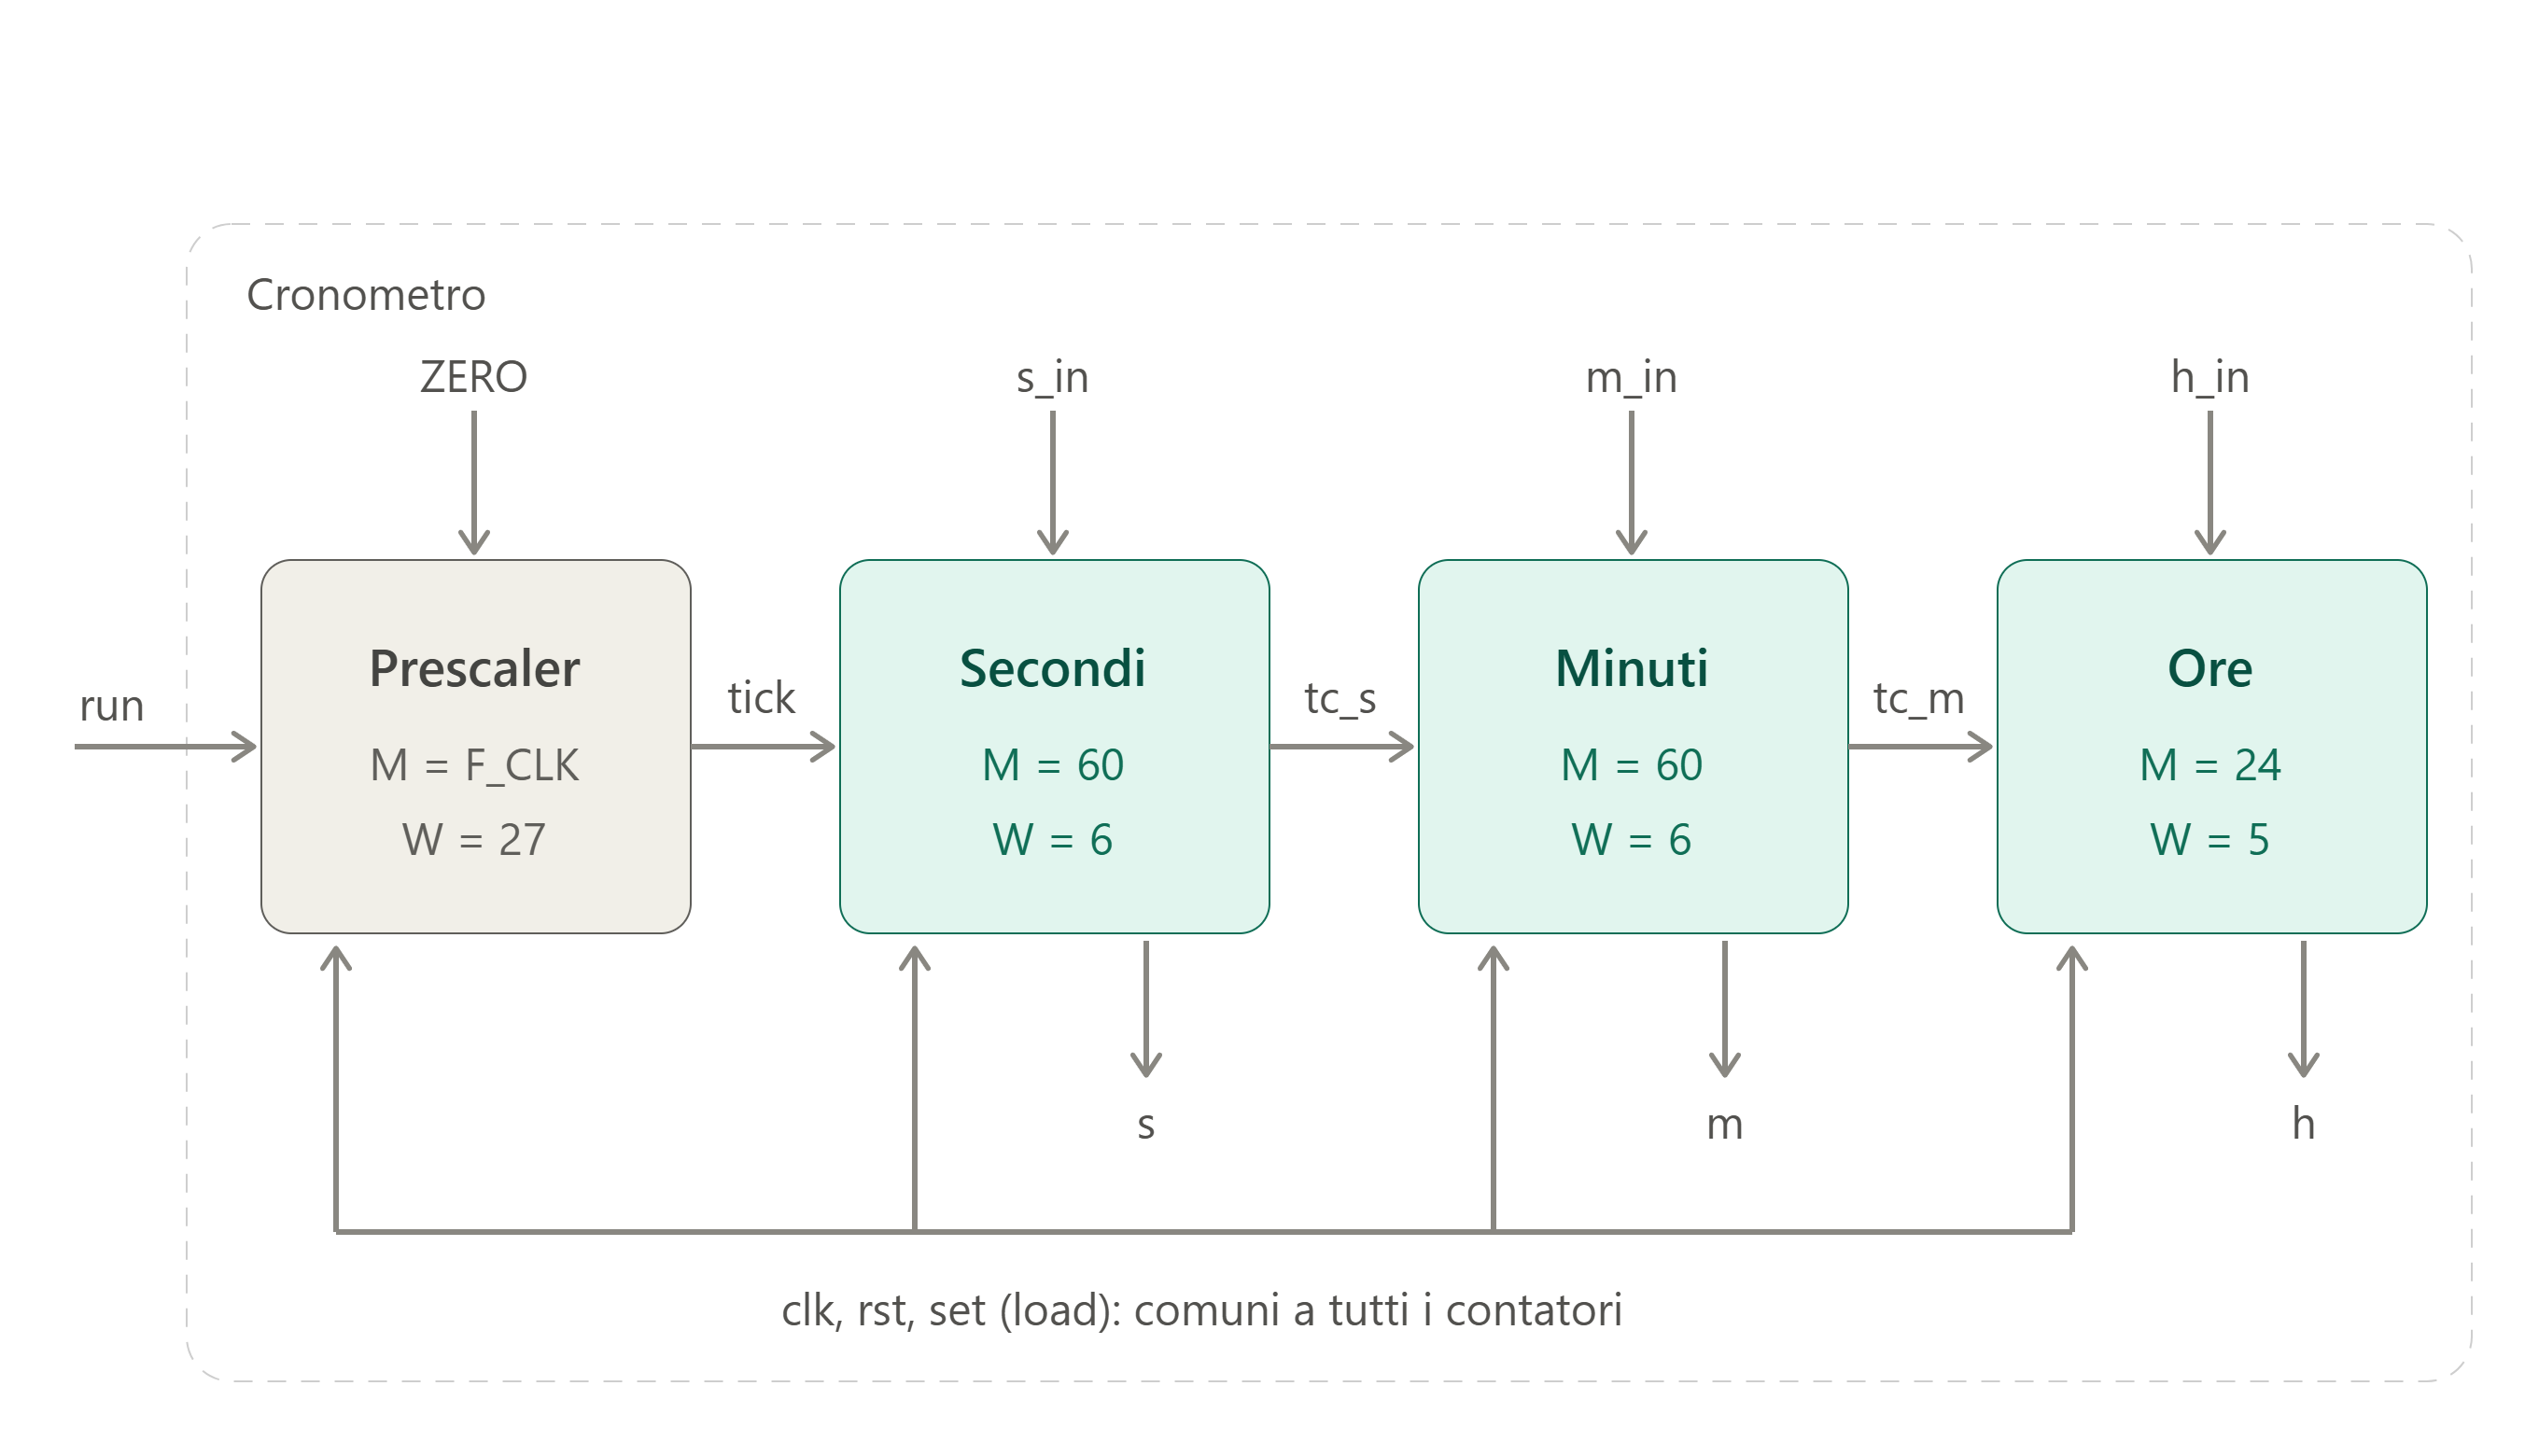
\includegraphics[width=0.7\linewidth]{figure/esercizio5-1/schema}
  \caption{Architettura del Cronometro}
  \label{fig:esercizio5-1:schema}
\end{figure}

Il valore iniziale è caricato tramite l'ingresso \texttt{load} dei contatori, collegato a \texttt{set}: ogni contatore riceve la propria parte del valore (\texttt{s\_in}, \texttt{m\_in}, \texttt{h\_in}), mentre il prescaler carica una costante nulla, così da ripartire dall'inizio del secondo.


\implementazione

Presentiamo per primo il contatore modulare \texttt{counter\_mod}, componente comune. I generic sono \texttt{M}, il modulo, e \texttt{W}, il numero di bit dell'uscita. Le porte sono \texttt{clk}, \texttt{rst} (reset sincrono), \texttt{en} (abilitazione al conteggio), \texttt{load} (caricamento del valore \texttt{d}), il dato \texttt{d} e l'uscita \texttt{q} a \texttt{W} bit, e infine il riporto \texttt{tc}. L'architettura è \texttt{behavioral}: un solo process sensibile a \texttt{clk} aggiorna il segnale interno \texttt{cnt}, con priorità decrescente a reset, caricamento e incremento; al raggiungimento di \texttt{M-1} il conteggio riparte da zero. Un \texttt{assert} con severità \texttt{failure} segnala il caso in cui \texttt{M} non è rappresentabile su \texttt{W} bit. Il riporto \texttt{tc} vale \texttt{'1'} quando \texttt{en} è attivo e il conteggio è a \texttt{M-1}, ossia quando al fronte successivo il contatore si azzera.

\vhdlfile{esercizio5-1/counter_mod.vhd}{Implementazione del Contatore modulare}{lst:esercizio5-1:counter-mod}

Definito tale componente, si riporta il top module \texttt{cronometro}. Il generic \texttt{F\_CLK}, di default 100\,000\,000, è il numero di cicli di clock per secondo. Le porte sono \texttt{clk}, \texttt{rst}, \texttt{run}, \texttt{set}, gli ingressi di inizializzazione \texttt{h\_in} (5 bit), \texttt{m\_in} e \texttt{s\_in} (6 bit) e le uscite \texttt{h}, \texttt{m}, \texttt{s} con le stesse larghezze. L'architettura è \texttt{structural}: la costante \texttt{W\_PRESC}, pari a 27, dimensiona il prescaler perché $2^{27}$ supera 100\,000\,000, mentre i segnali \texttt{tick}, \texttt{tc\_s} e \texttt{tc\_m} realizzano la cascata. Le quattro istanze \texttt{presc}, \texttt{sec}, \texttt{min} e \texttt{ore} sono create con port mapping e generic map; l'uscita \texttt{q} del prescaler e il riporto delle ore non sono utilizzati (\texttt{open}).

\vhdlfile{esercizio5-1/cronometro.vhd}{Implementazione del Cronometro}{lst:esercizio5-1:cronometro}

\simulazione

Il testbench \texttt{cronometro\_tb} ha entità senza porte e istanzia il top module come \texttt{dut}. Ai fini della simulazione \texttt{F\_CLK} è posto a 4: con un clock di periodo \texttt{T} di \SI{10}{ns}, un secondo corrisponde a \texttt{SEC} $= 4T = \SI{40}{ns}$. Il process \texttt{clk\_proc} genera il clock e \texttt{stim} applica la sequenza di stimoli, riportata di seguito.

\vhdlfile{esercizio5-1/cronometro_tb.vhd}{Testbench del Cronometro}{lst:esercizio5-1:cronometro-tb}

I passi del test sono i seguenti.
\begin{enumerate}
  \item Reset per due periodi di clock, poi \texttt{run} a \texttt{'1'} per cinque secondi: il tempo passa da 00:00:00 a 00:00:05.
  \item \texttt{run} a \texttt{'0'} per tre secondi: il conteggio resta fermo.
  \item Caricamento di 00:00:58 con un impulso di \texttt{set} e tre secondi di conteggio, fino a 00:01:00.
  \item Caricamento di 00:59:58, per verificare il riporto sulle ore (01:00:00).
  \item Caricamento di 23:59:58, per verificare il ritorno a 00:00:00 dopo 23:59:59.
  \item Impulso di \texttt{rst} e altri due secondi di conteggio.
\end{enumerate}

Il risultato della simulazione è mostrato in figura~\ref{fig:esercizio5-1:simulazione}.

\begin{figure}[H]
  \centering
  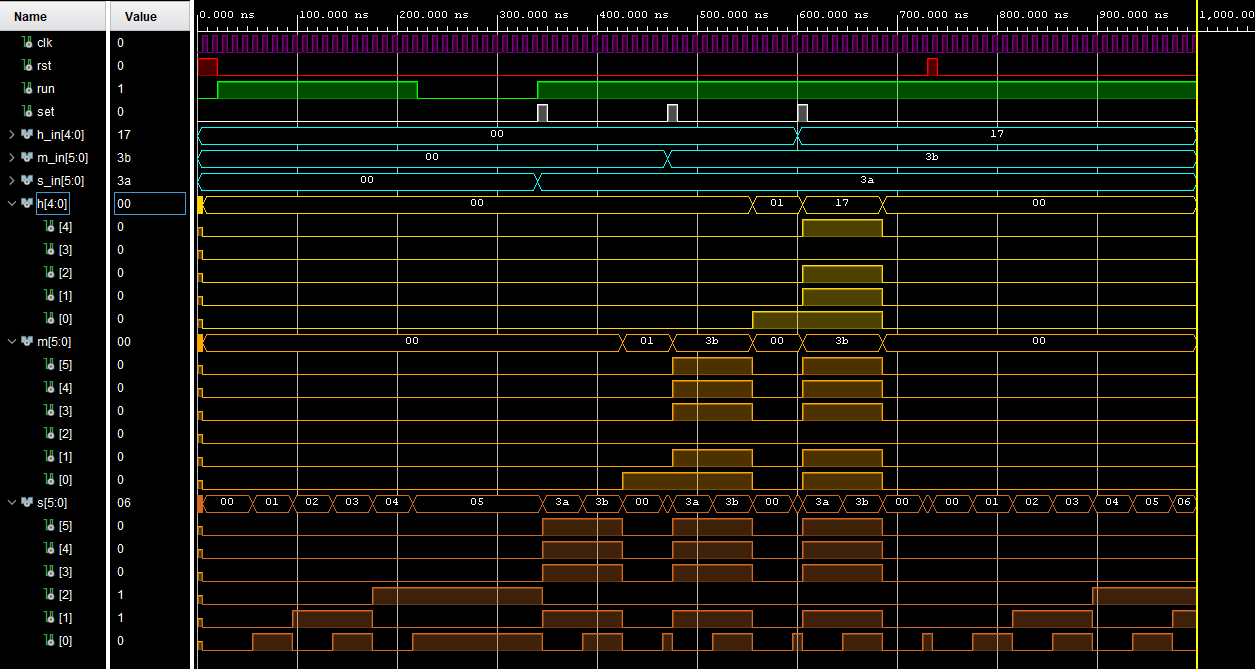
\includegraphics[width=\linewidth]{figure/esercizio5-1/simulazione}
  \caption{Simulazione del Cronometro}
  \label{fig:esercizio5-1:simulazione}
\end{figure}

Consideriamo il caricamento di 23:59:58. Con \texttt{h\_in} $=$ 0x17 ($10111_2$, ossia $23_{10}$), \texttt{m\_in} $=$ 0x3B ($59_{10}$) e \texttt{s\_in} $=$ 0x3A ($58_{10}$), un impulso di \texttt{set} porta le uscite a \texttt{h} $=$ 17, \texttt{m} $=$ 3b, \texttt{s} $=$ 3a. Dopo un secondo \texttt{s} vale 3b (59), dopo un altro secondo si azzera e il riporto propaga l'azzeramento a \texttt{m} e a \texttt{h}: le uscite tornano a 00:00:00. Nel caricamento precedente (00:59:58) l'ora passa da 00 a 01 e i minuti da 3b a 00. Dopo l'impulso di \texttt{rst} tutte le uscite sono a zero e il conteggio riprende dai secondi, che nell'ultima parte della figura arrivano a 06.

\begin{risultato}
La simulazione verifica il comportamento alle transizioni critiche (cambio di minuto, ora, giorno), l'arresto quando \texttt{run} è inattivo e l'azzeramento con \texttt{rst}.
\end{risultato}

\esSezione{Cronometro su board}\label{sec:esercizio5-2}

\begin{traccia}
Sintetizzare ed implementare su board il componente sviluppato al punto precedente, utilizzando i display a 7 segmenti per la visualizzazione dell'orario (o una combinazione di display e led nel caso in cui i display a disposizione siano in numero inferiore a quello necessario), gli switch per l'immissione dell'orario iniziale e due bottoni, uno per il set dell'orario e uno per il reset. Si utilizzi una codifica a scelta dello studente per la visualizzazione dell'orario sui display (esadecimale o decimale).
\end{traccia}

\progetto

Il cronometro dell'esercizio~\ref{sec:esercizio5-1} viene mantenuto invariato (listati~\ref{lst:esercizio5-1:cronometro} e~\ref{lst:esercizio5-1:counter-mod}); il top module gli affianca quattro blocchi.

\begin{enumerate}
  \item il \texttt{debouncer}, già presentato nell'esercizio~\ref{sec:esercizio3-2} (listato~\ref{lst:esercizio3-2:debouncer}), che ripulisce il bottone centrale;
  \item l'\texttt{input\_manager}, che acquisisce ore, minuti e secondi iniziali attraverso un unico gruppo di sei switch;
  \item tre istanze di \texttt{bin2dec}, che convertono i valori binari di ore, minuti e secondi in due cifre BCD ciascuna;
  \item il \texttt{display\_driver}, che pilota in multiplexing i display a 7 segmenti e al suo interno usa il decodificatore \texttt{seg7\_decoder}.
\end{enumerate}

Per l'orario iniziale servono $5+6+6=17$ bit, più dei 16 switch della board. Si è scelto di inserire i tre campi uno alla volta, con gli stessi sei switch \texttt{SW(5:0)}, e di confermarli con una sequenza di pressioni del bottone centrale: la prima carica le ore, la seconda i minuti, la terza i secondi e genera il \texttt{set} del cronometro. I tre LED \texttt{LED(2:0)} indicano il campo in attesa di essere caricato. Il bottone inferiore \texttt{BTND} è il reset, mentre lo switch \texttt{SW(15)} è collegato all'ingresso \texttt{run} e avvia o ferma il conteggio. L'orario è mostrato in decimale su sei delle otto cifre disponibili, nella forma ore, minuti, secondi.

\implementazione

Presentiamo per primo il convertitore \texttt{bin2dec}. L'ingresso \texttt{bin} è a 6 bit (valori 0--63) e le uscite \texttt{decine} e \texttt{unita} sono due cifre BCD a 4 bit. L'architettura è \texttt{behavioral}: un process sensibile a \texttt{v}, copia unsigned di \texttt{bin}, confronta il valore con le soglie 60, 50, \ldots, 10 in una catena di \texttt{if}/\texttt{elsif}, assegna la cifra delle decine e sottrae la soglia per ottenere le unità. Così si evitano i divisori: basta un comparatore per soglia.

\vhdlfile{esercizio5-2/bin2dec.vhd}{Implementazione del convertitore binario-BCD}{lst:esercizio5-2:bin2dec}

Il decodificatore \texttt{seg7\_decoder} ha un ingresso \texttt{cifra} a 4 bit e un'uscita \texttt{seg} a 7 bit, nell'ordine \texttt{gfedcba}, attiva bassa come i segmenti della board. L'architettura \texttt{dataflow} usa un'unica assegnazione \texttt{with select}; ogni valore non compreso tra 0 e 9 spegne tutti i segmenti.

\vhdlfile{esercizio5-2/seg7_decoder.vhd}{Implementazione del decodificatore a 7 segmenti}{lst:esercizio5-2:seg7-decoder}

Il \texttt{display\_driver} ha il generic \texttt{N\_REFRESH}, di default 100\,000 cicli di clock, pari a \SI{1}{ms} a \SI{100}{MHz}. Gli ingressi sono \texttt{clk}, \texttt{rst} e le sei cifre BCD \texttt{ore\_d}, \texttt{ore\_u}, \texttt{min\_d}, \texttt{min\_u}, \texttt{sec\_d}, \texttt{sec\_u}; le uscite sono \texttt{seg} (7 bit), \texttt{dp} e \texttt{an} (8 bit), tutte attive basse. L'architettura è \texttt{structural} e riusa il contatore modulare: l'istanza \texttt{refresh} (modulo \texttt{N\_REFRESH}, 17 bit) produce un impulso \texttt{tick} ogni millisecondo, mentre \texttt{sel\_cnt} (modulo 6, 3 bit) avanza di una posizione a ogni \texttt{tick} e fornisce il segnale \texttt{sel}. Un process combinatorio, sensibile a \texttt{sel} e alle sei cifre, seleziona la cifra da mostrare, l'anodo da accendere e lo stato del punto decimale, che resta acceso sulle cifre delle unità di ore e di minuti per separare i tre campi. Un solo \texttt{seg7\_decoder} serve tutte le cifre; le due restanti non sono mai selezionate e restano spente.

\vhdlfile{esercizio5-2/display_driver.vhd}{Implementazione del Display Driver}{lst:esercizio5-2:display-driver}

L'\texttt{input\_manager} ha come ingressi \texttt{clk}, \texttt{rst}, \texttt{load} (il segnale proveniente dal debouncer) e \texttt{sw}, a 6 bit. Le uscite sono \texttt{h\_in} (5 bit), \texttt{m\_in} e \texttt{s\_in} (6 bit), l'impulso \texttt{set} e \texttt{campo} (3 bit) per i LED. L'architettura \texttt{behavioral} è una FSM a tre stati, \texttt{ORE}, \texttt{MINUTI} e \texttt{SECONDI}, descritta con un solo process sincrono: a ogni \texttt{load} il valore degli switch viene memorizzato nel registro del campo corrente e lo stato avanza; nello stato \texttt{SECONDI}, inoltre, \texttt{set} viene posto a \texttt{'1'} per un ciclo e la macchina torna in \texttt{ORE}. Il reset sincrono azzera i registri e riporta la macchina in \texttt{ORE}. L'uscita \texttt{campo} vale \texttt{"100"}, \texttt{"010"} o \texttt{"001"} a seconda dello stato.

\vhdlfile{esercizio5-2/input_manager.vhd}{Implementazione dell'Input Manager}{lst:esercizio5-2:input-manager}

Il top module \texttt{cronometro\_tl} (nel file \texttt{coronometro\_tl.vhd}) ha le porte coerenti con i nomi dei vincoli della board: \texttt{CLK100MHZ}, \texttt{SW} (16 bit), \texttt{BTNC}, \texttt{BTND}, \texttt{LED} (3 bit), i sette segmenti \texttt{CA}--\texttt{CG}, \texttt{DP} e \texttt{AN} (8 bit). L'architettura è \texttt{structural}. Il reset \texttt{rst} è collegato direttamente a \texttt{BTND}, mentre \texttt{BTNC} attraversa il \texttt{debouncer} e produce \texttt{load\_p}. Questo alimenta l'\texttt{input\_manager}, la cui uscita \texttt{set\_p} e i valori \texttt{h\_in}, \texttt{m\_in}, \texttt{s\_in} entrano nel \texttt{cronometro}, con \texttt{run} collegato a \texttt{SW(15)}. Le ore, estese a 6 bit con uno zero in testa (\texttt{h\_ext}), e i minuti e secondi passano per le tre istanze \texttt{conv\_h}, \texttt{conv\_m} e \texttt{conv\_s} di \texttt{bin2dec}; le sei cifre risultanti raggiungono il \texttt{display\_driver}. Il vettore \texttt{seg} è poi scomposto nei singoli segnali \texttt{CA}--\texttt{CG}.

\vhdlfile{esercizio5-2/coronometro_tl.vhd}{Implementazione del top module Cronometro su board}{lst:esercizio5-2:coronometro-tl}

Per questo esercizio non è stato sviluppato un testbench: il comportamento è verificato direttamente sulla scheda.

\sintesiboard

Il circuito è stato sintetizzato ed implementato sulla Nexys A7-100T. Dopo il reset con \texttt{BTND}, si impostano gli switch \texttt{SW(5:0)} sul valore delle ore e si preme \texttt{BTNC}; si ripete l'operazione per minuti e secondi, controllando sui LED il campo in corso. Alla terza pressione l'orario impostato viene caricato nel cronometro e, con \texttt{SW(15)} alto, il conteggio procede. Nella figura~\ref{fig:esercizio5-2:board} sono mostrati i display in due momenti: nella foto (a) compaiono ore, minuti e secondi con le cifre accese, nella foto (b) l'orario azzerato, con i punti decimali che separano i tre campi.

\begin{figure}[H]
  \centering
  \begin{subfigure}[b]{0.45\linewidth}
    \centering
    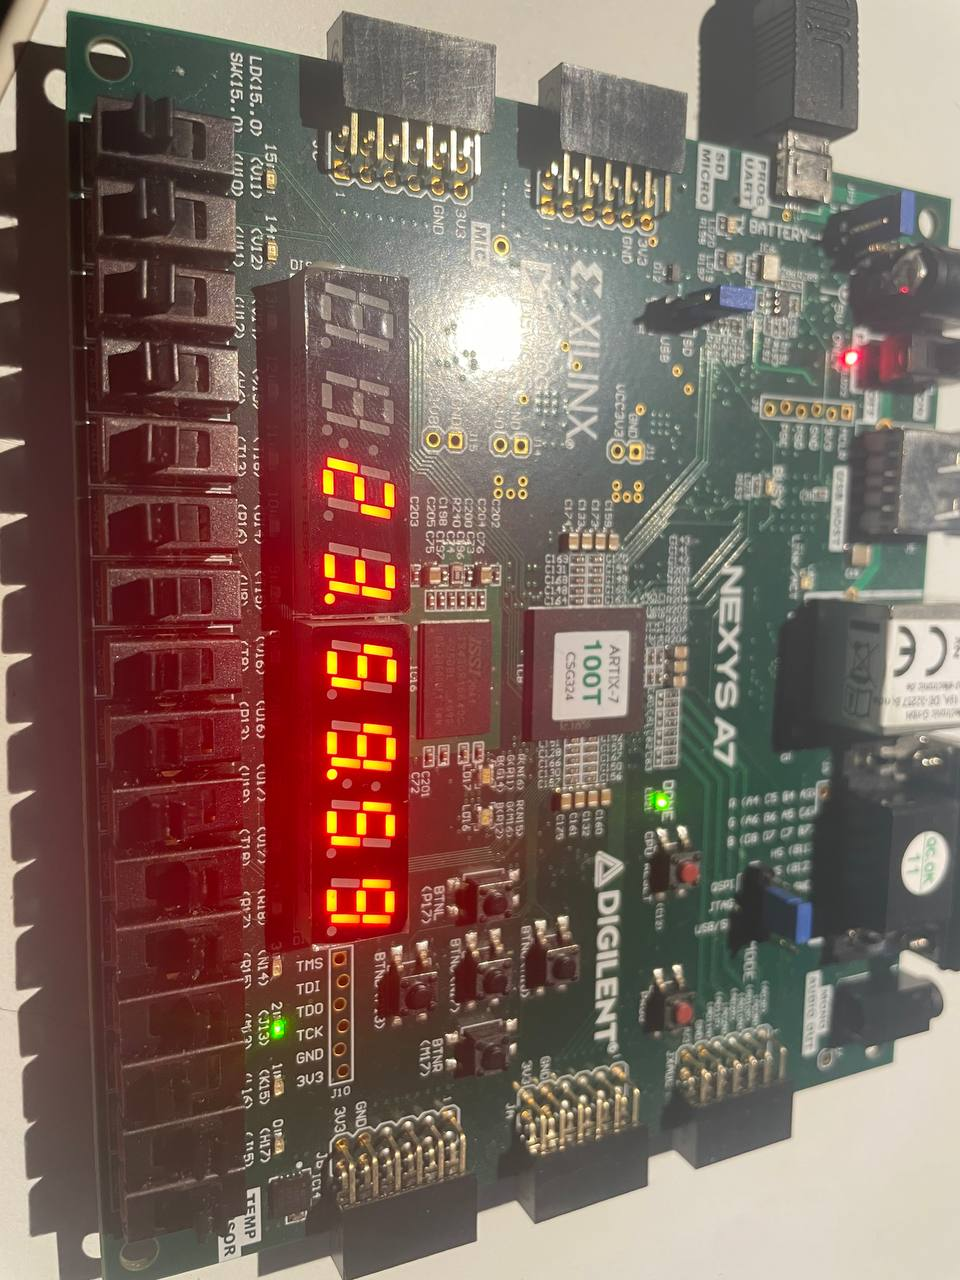
\includegraphics[width=\linewidth]{figure/esercizio5-2/board-1}
    \caption{Orario in corso}
  \end{subfigure}
  \hfill
  \begin{subfigure}[b]{0.45\linewidth}
    \centering
    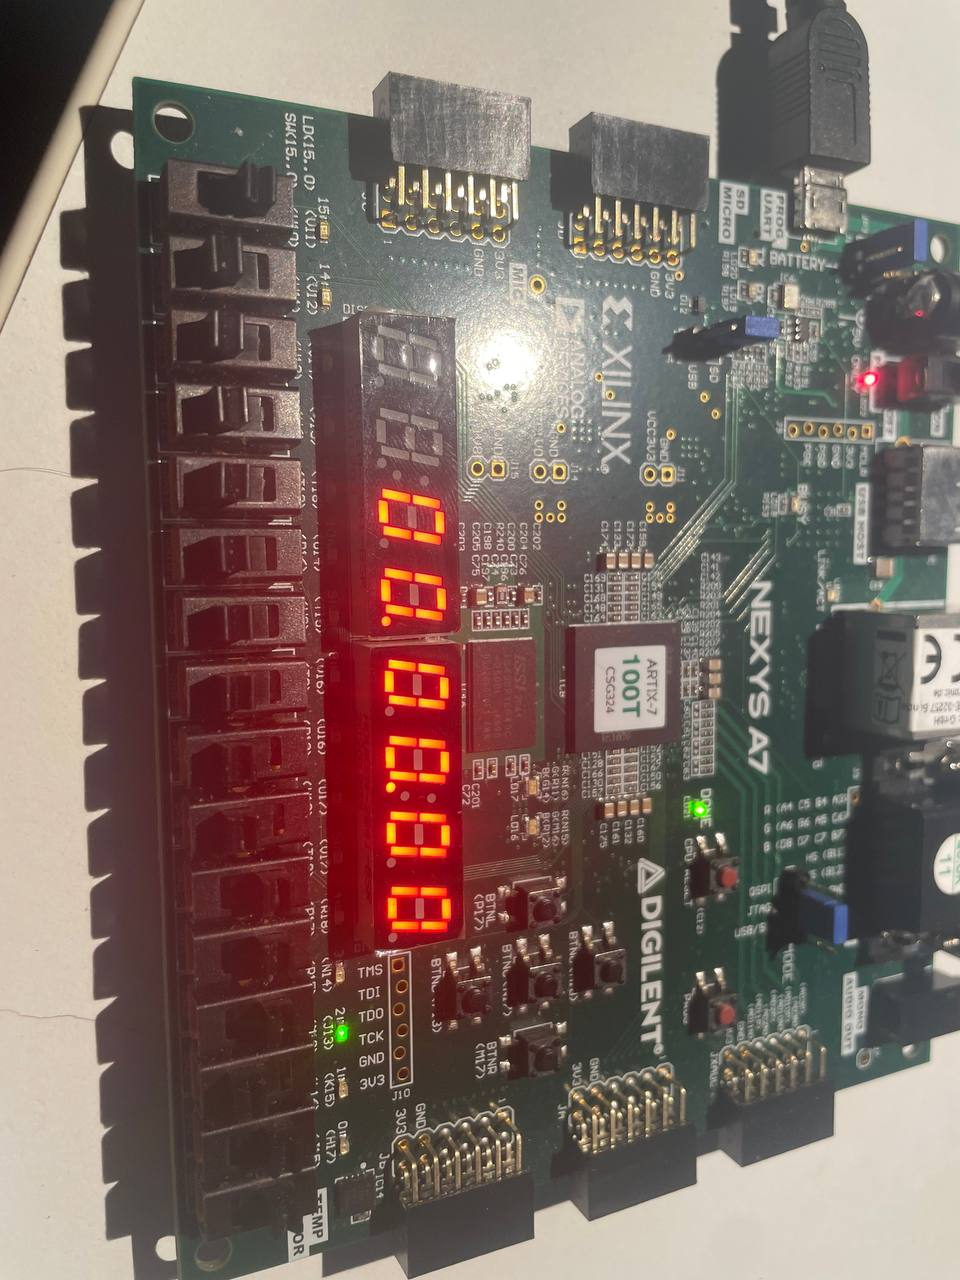
\includegraphics[width=\linewidth]{figure/esercizio5-2/board-2}
    \caption{Orario azzerato}
  \end{subfigure}
  \caption{Cronometro su Board}
  \label{fig:esercizio5-2:board}
\end{figure}

Nel file dei constraint sono state decommentate le seguenti righe.

\xdcfile{esercizio5-2/vincoli.xdc}{Constraint}{lst:esercizio5-2:vincoli}


\esCapitolo{Sistema di lettura, elaborazione e scrittura}\label{cap:po-pc}
\esSezione{Sistema PO/PC}\label{sec:esercizio6-1}

\begin{traccia}
Progettare, implementare in VHDL e verificare mediante simulazione un sistema dotato di una memoria ROM di N locazioni da 8 bit ciascuna, una macchina combinatoria M in grado di trasformare (secondo una funzione a scelta dello studente) la stringa di 8 bit letta dalla ROM in una stringa di 4 bit, e una memoria MEM di N locazioni che memorizza la stringa in output da M.

Il sistema si avvia in corrispondenza di un segnale di START che viene fornito esternamente. Una volta avviato, tramite un'apposita unità di controllo che gestisce la tempificazione del sistema, viene scandita una locazione alla volta della ROM e viene scritta la corrispondente locazione di MEM. Gli indirizzi di memoria sono forniti da un contatore. Le memorie ROM e MEM hanno rispettivamente un read e un write sincrono.
\end{traccia}


\progetto

Il sistema si divide in parte operativa e parte di controllo. Il top module \texttt{sistema} istanzia cinque componenti:
\begin{enumerate}
  \item Control Unit (\texttt{control\_unit});
  \item ROM (\texttt{rom});
  \item macchina combinatoria $M$ (\texttt{onecount});
  \item memoria (\texttt{mem});
  \item contatore (\texttt{counter\_mod}).
\end{enumerate}

L'indirizzo, comune a ROM e MEM, è fornito dal contatore. La ROM restituisce il byte letto su \texttt{rom\_data}; la macchina $M$ lo trasforma in \texttt{m\_data}, che è il dato in ingresso alla MEM. L'unità di controllo riceve \texttt{start} e il riporto \texttt{tc} del contatore e produce i comandi \texttt{rd} (lettura della ROM), \texttt{we} (scrittura della MEM), \texttt{cnt\_en} (avanzamento del contatore) e l'uscita \texttt{done}. La funzione scelta per $M$ è il conteggio degli '1' presenti nel byte, così il risultato, compreso tra 0 e 8, sta su 4 bit.

Lo schema a blocchi dell'architettura è riportato in Figura~\ref{fig:esercizio6-1:schema}: in basso la parte operativa, in alto l'unità di controllo con i segnali di controllo e di stato scambiati con essa.

\begin{figure}[H]
  \centering
  \scalebox{0.93}{%
  \begin{tikzpicture}[font=\sffamily\small]
    \node[blocco, minimum width=1.8cm] (cnt) at (0,0) {\texttt{counter\_mod}};
    \node[blocco, minimum width=1.8cm] (rom) at (4,0) {\texttt{rom}};
    \node[blocco, minimum width=1.8cm] (m) at (8,0) {$M$\\[-2pt]\scriptsize\texttt{onecount}};
    \node[blocco, minimum width=1.8cm] (mem) at (12,0) {\texttt{mem}};
    \node[ctrl, minimum width=6.5cm] (cu) at (6,3.2) {\texttt{control\_unit}};

    \draw[bus] (cnt) -- node[pos=0.25, above=3pt, font=\scriptsize]{\texttt{addr}} node[pos=0.55, sloped, inner sep=1pt]{/} node[pos=0.55, below=3pt, font=\scriptsize]{4} (rom);
    \draw[bus] (rom) -- node[pos=0.28, above=3pt, font=\scriptsize]{\texttt{rom\_data}} node[pos=0.75, sloped, inner sep=1pt]{/} node[pos=0.75, below=3pt, font=\scriptsize]{8} (m);
    \draw[bus] (m) -- node[pos=0.28, above=3pt, font=\scriptsize]{\texttt{m\_data}} node[pos=0.75, sloped, inner sep=1pt]{/} node[pos=0.75, below=3pt, font=\scriptsize]{4} (mem);
    \draw[bus] (2.8,0) -- (2.8,-1.2) -- node[below, font=\scriptsize]{\texttt{addr} ($\to$ \texttt{waddr})} (11.6,-1.2) -- (11.6,-0.5);
    \fill (2.8,0) circle (1.5pt);
    \draw[bus,<-] (12.4,-0.5) -- (12.4,-1.2) node[below, font=\scriptsize]{\texttt{raddr}};
    \draw[bus] (mem.east) -- ++(1,0) node[right, font=\scriptsize]{\texttt{dout}};

    \draw[seg] ([xshift=-3cm]cu.south) -- ++(0,-0.6) -| (cnt.north);
    \node[font=\scriptsize, left] at (2.9,2.3) {\texttt{cnt\_en}};
    \draw[seg] ([xshift=-1cm]cu.south) -- ++(0,-0.9) -| (rom.north);
    \node[font=\scriptsize, right] at (5.1,2.1) {\texttt{rd}};
    \draw[seg] ([xshift=3cm]cu.south) -- ++(0,-0.6) -| (mem.north);
    \node[font=\scriptsize, right] at (9.1,2.3) {\texttt{we}};
    \draw[seg] (cnt.west) -- ++(-0.7,0) |- node[pos=0.25, left, font=\scriptsize]{\texttt{tc}} (cu.west);
    \draw[seg,<-] ([xshift=-0.8cm]cu.north) -- ++(0,0.6) node[above, font=\scriptsize]{\texttt{start}};
    \draw[seg,<-] ([xshift=0.8cm]cu.north) -- ++(0,0.6) node[above, font=\scriptsize]{\texttt{rst}};
    \draw[seg] (cu.east) -- ++(1,0) node[right, font=\scriptsize]{\texttt{done}};
  \end{tikzpicture}}
  \caption{Architettura PO/PC del sistema. \texttt{clk} raggiunge tutti i blocchi sincroni e \texttt{rst} anche il contatore; non sono disegnati.}
  \label{fig:esercizio6-1:schema}
\end{figure}

\implementazione

Partiamo dai componenti della parte operativa. La ROM è descritta dall'entità \texttt{rom}, con generic \texttt{N} (locazioni) e \texttt{A} (bit di indirizzo) e porte \texttt{clk}, \texttt{rd}, \texttt{addr} (\texttt{A} bit) e \texttt{data} (8 bit). L'architettura \texttt{behavioral} contiene la costante \texttt{CONTENT}, un array di \texttt{N} byte con sedici valori iniziali e gli altri a \texttt{x"00"}. Un process sensibile a \texttt{clk} carica \texttt{data} sul fronte di salita solo se \texttt{rd} vale '1', quindi la lettura è sincrona. Un \texttt{assert} con severità \texttt{failure} controlla che \texttt{N} sia indirizzabile su \texttt{A} bit. 

\vhdlfile{esercizio6-1/rom.vhd}{Implementazione della ROM}{lst:esercizio6-1:rom}

La macchina combinatoria $M$ è l'entità \texttt{onecount}, con ingresso \texttt{x} a 8 bit e uscita \texttt{y} a 4 bit. Un process sensibile a \texttt{x} azzera una variabile \texttt{n} di tipo \texttt{unsigned} e la incrementa per ogni bit di \texttt{x} pari a '1', con un ciclo \texttt{for} sugli otto indici; \texttt{y} è il risultato convertito in \texttt{std\_logic\_vector}. Senza clock, la rete è puramente combinatoria.

\vhdlfile{esercizio6-1/onecount.vhd}{Implementazione della macchina combinatoria $M$ (conteggio degli '1')}{lst:esercizio6-1:onecount}

L'entità \texttt{mem} ha generic \texttt{N}, \texttt{A} e \texttt{W} (larghezza del dato, 4 per default) e porte \texttt{clk}, \texttt{we}, \texttt{waddr}, \texttt{din}, oltre a \texttt{raddr} e \texttt{dout}, aggiunte per consentire al testbench di leggere il contenuto. La scrittura avviene in un process sincrono, quando \texttt{we} vale '1'; la lettura su \texttt{dout} è invece un assegnamento concorrente, quindi asincrona. Le locazioni sono inizializzate a tutti '1'. La MEM espone quindi anche un'uscita.

\vhdlfile{esercizio6-1/mem.vhd}{Implementazione della memoria MEM}{lst:esercizio6-1:mem}

Il contatore è \texttt{counter\_mod}, già presentato nell'esercizio 5.1 (listato~\ref{lst:esercizio5-1:counter-mod}). Nel sistema è istanziato con \texttt{M} pari a \texttt{N} e \texttt{W} pari a \texttt{A}, con \texttt{load} a '0' e ingresso \texttt{d} a zero; l'uscita \texttt{tc} vale '1' quando il contatore è abilitato e si trova sull'ultimo valore.

L'unità di controllo \texttt{control\_unit} è una FSM di tipo Moore con quattro stati (\texttt{S\_IDLE}, \texttt{S\_READ}, \texttt{S\_WRITE}, \texttt{S\_DONE}), descritta con due process. Il process \texttt{f\_controllo}, sensibile a \texttt{stato\_corrente}, \texttt{start} e \texttt{tc}, assegna dei valori di default alle uscite e calcola lo stato prossimo; il process \texttt{mem\_stato} aggiorna \texttt{stato\_corrente} sul fronte di salita di \texttt{clk}, con reset sincrono verso \texttt{S\_IDLE}. Gli stati si comportano così:
\begin{enumerate}
  \item in \texttt{S\_IDLE} si attende \texttt{start} a '1' per passare in \texttt{S\_READ};
  \item in \texttt{S\_READ} viene attivato \texttt{rd} e si passa in \texttt{S\_WRITE};
  \item in \texttt{S\_WRITE} vengono attivati \texttt{we} e \texttt{cnt\_en}; se \texttt{tc} vale '1' si va in \texttt{S\_DONE}, altrimenti si torna in \texttt{S\_READ};
  \item in \texttt{S\_DONE} viene attivato \texttt{done}, e si torna in \texttt{S\_IDLE} solo quando \texttt{start} torna a '0'.
\end{enumerate}
Ogni locazione richiede quindi due cicli di clock: nel primo la ROM campiona l'indirizzo, nel secondo il dato elaborato da $M$ è disponibile e viene scritto in MEM nello stesso fronte in cui il contatore avanza. 

\vhdlfile{esercizio6-1/control_unit.vhd}{Implementazione della Control Unit}{lst:esercizio6-1:cu}

Il top module \texttt{sistema} ha generic \texttt{N} (16) e \texttt{A} (4) e porte \texttt{clk}, \texttt{rst}, \texttt{start} in ingresso, \texttt{done} in uscita, oltre a \texttt{raddr} e \texttt{dout} per la lettura della MEM. L'architettura \texttt{structural} istanzia i cinque componenti con port mapping e dichiara i segnali interni \texttt{addr}, \texttt{rom\_data}, \texttt{m\_data}, \texttt{rd}, \texttt{we}, \texttt{cnt\_en} e \texttt{tc}.

\vhdlfile{esercizio6-1/sistema.vhd}{Implementazione del top module del sistema}{lst:esercizio6-1:sistema}

\simulazione

Il testbench \texttt{sistema\_tb} ha un'entità senza porte e istanzia il top module come \texttt{dut} con \texttt{N} pari a 16 e \texttt{A} pari a 4. Il clock ha periodo di \SI{10}{ns}, generato da un process dedicato. Il process \texttt{stim} esegue questi passi:
\begin{itemize}
  \item \texttt{rst} a '1' per due periodi, poi a '0' per altri due;
  \item \texttt{start} a '1' e attesa di \texttt{done} a '1';
  \item attesa di tre periodi, poi \texttt{start} a '0' e altri due periodi;
  \item lettura di tutte le locazioni della MEM tramite \texttt{raddr}, con un \texttt{assert} per ciascuna, confrontata con i valori attesi della costante \texttt{EXP}, con severità \texttt{error}.
\end{itemize}
I valori attesi sono il numero di '1' di ciascun byte della ROM: $0, 8, 1, 1, 4, 4, 4, 4, 7, 7, 2, 4, 6, 1, 4, 4$.

\vhdlfile{esercizio6-1/sistema_tb.vhd}{Testbench del sistema}{lst:esercizio6-1:tb}

Il risultato della simulazione è in figura~\ref{fig:esercizio6-1:simulazione}.

\begin{figure}[H]
  \centering
  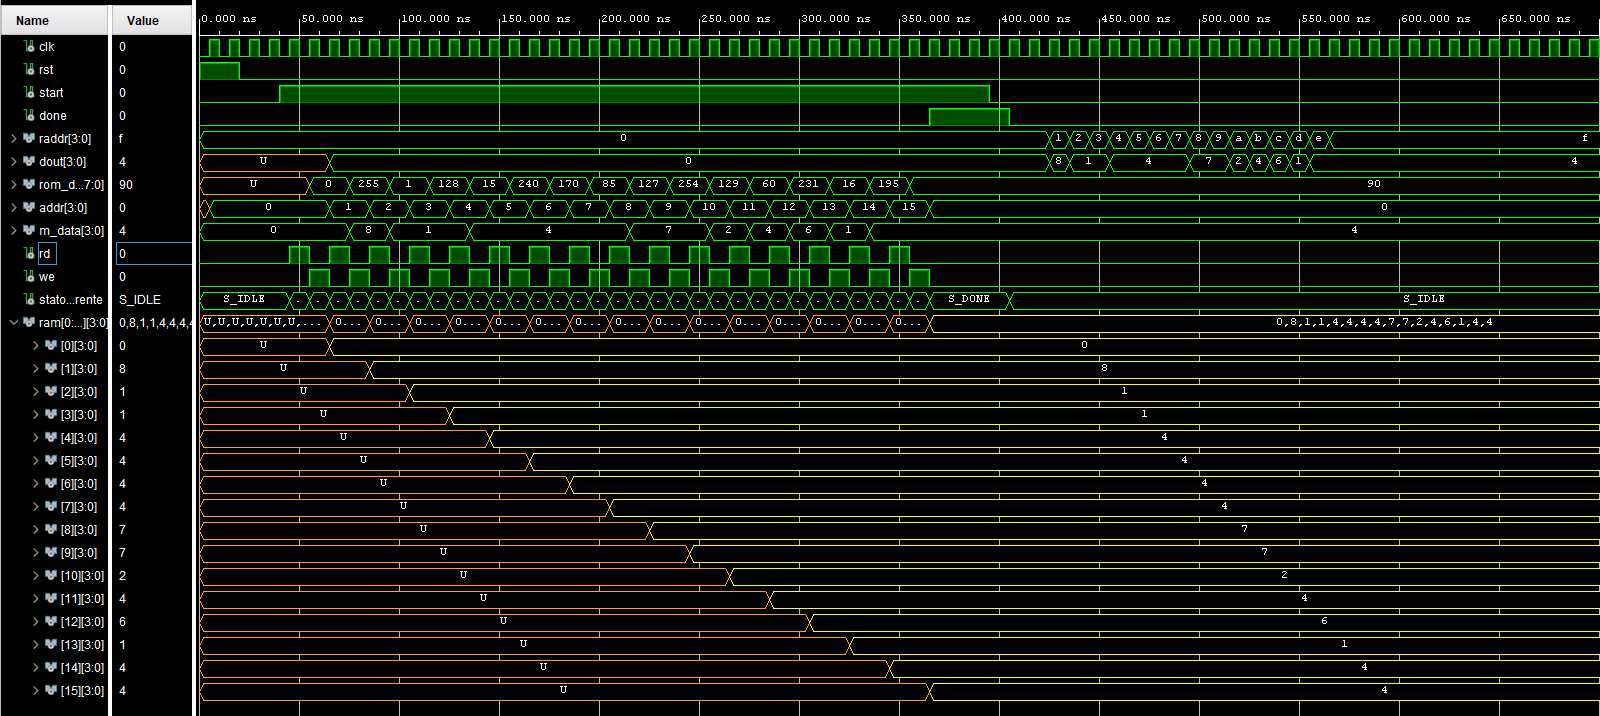
\includegraphics[width=\linewidth]{figure/esercizio6-1/simulazione}
  \caption{Simulazione del sistema PO/PC}
  \label{fig:esercizio6-1:simulazione}
\end{figure}


\begin{risultato}
Il contenuto finale di \texttt{ram} mostrato in figura coincide con i valori attesi di \texttt{EXP}, e \texttt{done} viene attivato una volta al termine della scansione.
\end{risultato}

\esercizioDaSvolgere{Sistema PO/PC su board}{esercizio6-2}

\esercizioDaSvolgere{Timing analysis del sistema PO/PC}{esercizio6-3}


\esCapitolo{Moltiplicatore di Booth}\label{cap:moltiplicatore-booth}
\esSezione{Moltiplicatore di Booth}\label{sec:esercizio7-1}

\begin{traccia}
Progettare, implementare in VHDL e testare mediante simulazione un moltiplicatore di Booth in grado di calcolare il prodotto di due stringhe da 8 bit, interpretate come numeri con segno in complemento a due.
\end{traccia}

\progetto

L'algoritmo di Booth moltiplica numeri con segno in complemento a due esaminando, a ogni passo, la coppia formata dal bit meno significativo del moltiplicatore e dal bit scartato al passo precedente. Detti \texttt{q0} e \texttt{qm1} tali bit, si hanno tre casi:

\begin{enumerate}
  \item se la coppia vale $00_2$ oppure $11_2$, viene eseguito soltanto lo shift aritmetico a destra;
  \item se vale $01_2$, il moltiplicando viene sommato alla parte alta del prodotto parziale, poi si effettua lo shift;
  \item se vale $10_2$, il moltiplicando viene sottratto alla parte alta, poi si effettua lo shift.
\end{enumerate}

Il calcolo richiede otto passi, uno per bit del moltiplicatore, e il sistema è diviso in parte operativa e unità di controllo. La parte operativa contiene il registro \texttt{M} (moltiplicando), il registro \texttt{A} (parte alta del prodotto parziale), il registro \texttt{Q} (moltiplicatore e parte bassa del prodotto), il flip-flop \texttt{Q[-1]}, un addizionatore/sottrattore a 8 bit e un contatore modulo 8 per contare i passi. L'unità di controllo è una FSM: produce i comandi per i registri e legge \texttt{q0}, \texttt{qm1} e \texttt{last}. Lo schema è visibile in figura~\ref{fig:esercizio7-1:schema}.

\begin{figure}[H]
  \centering
  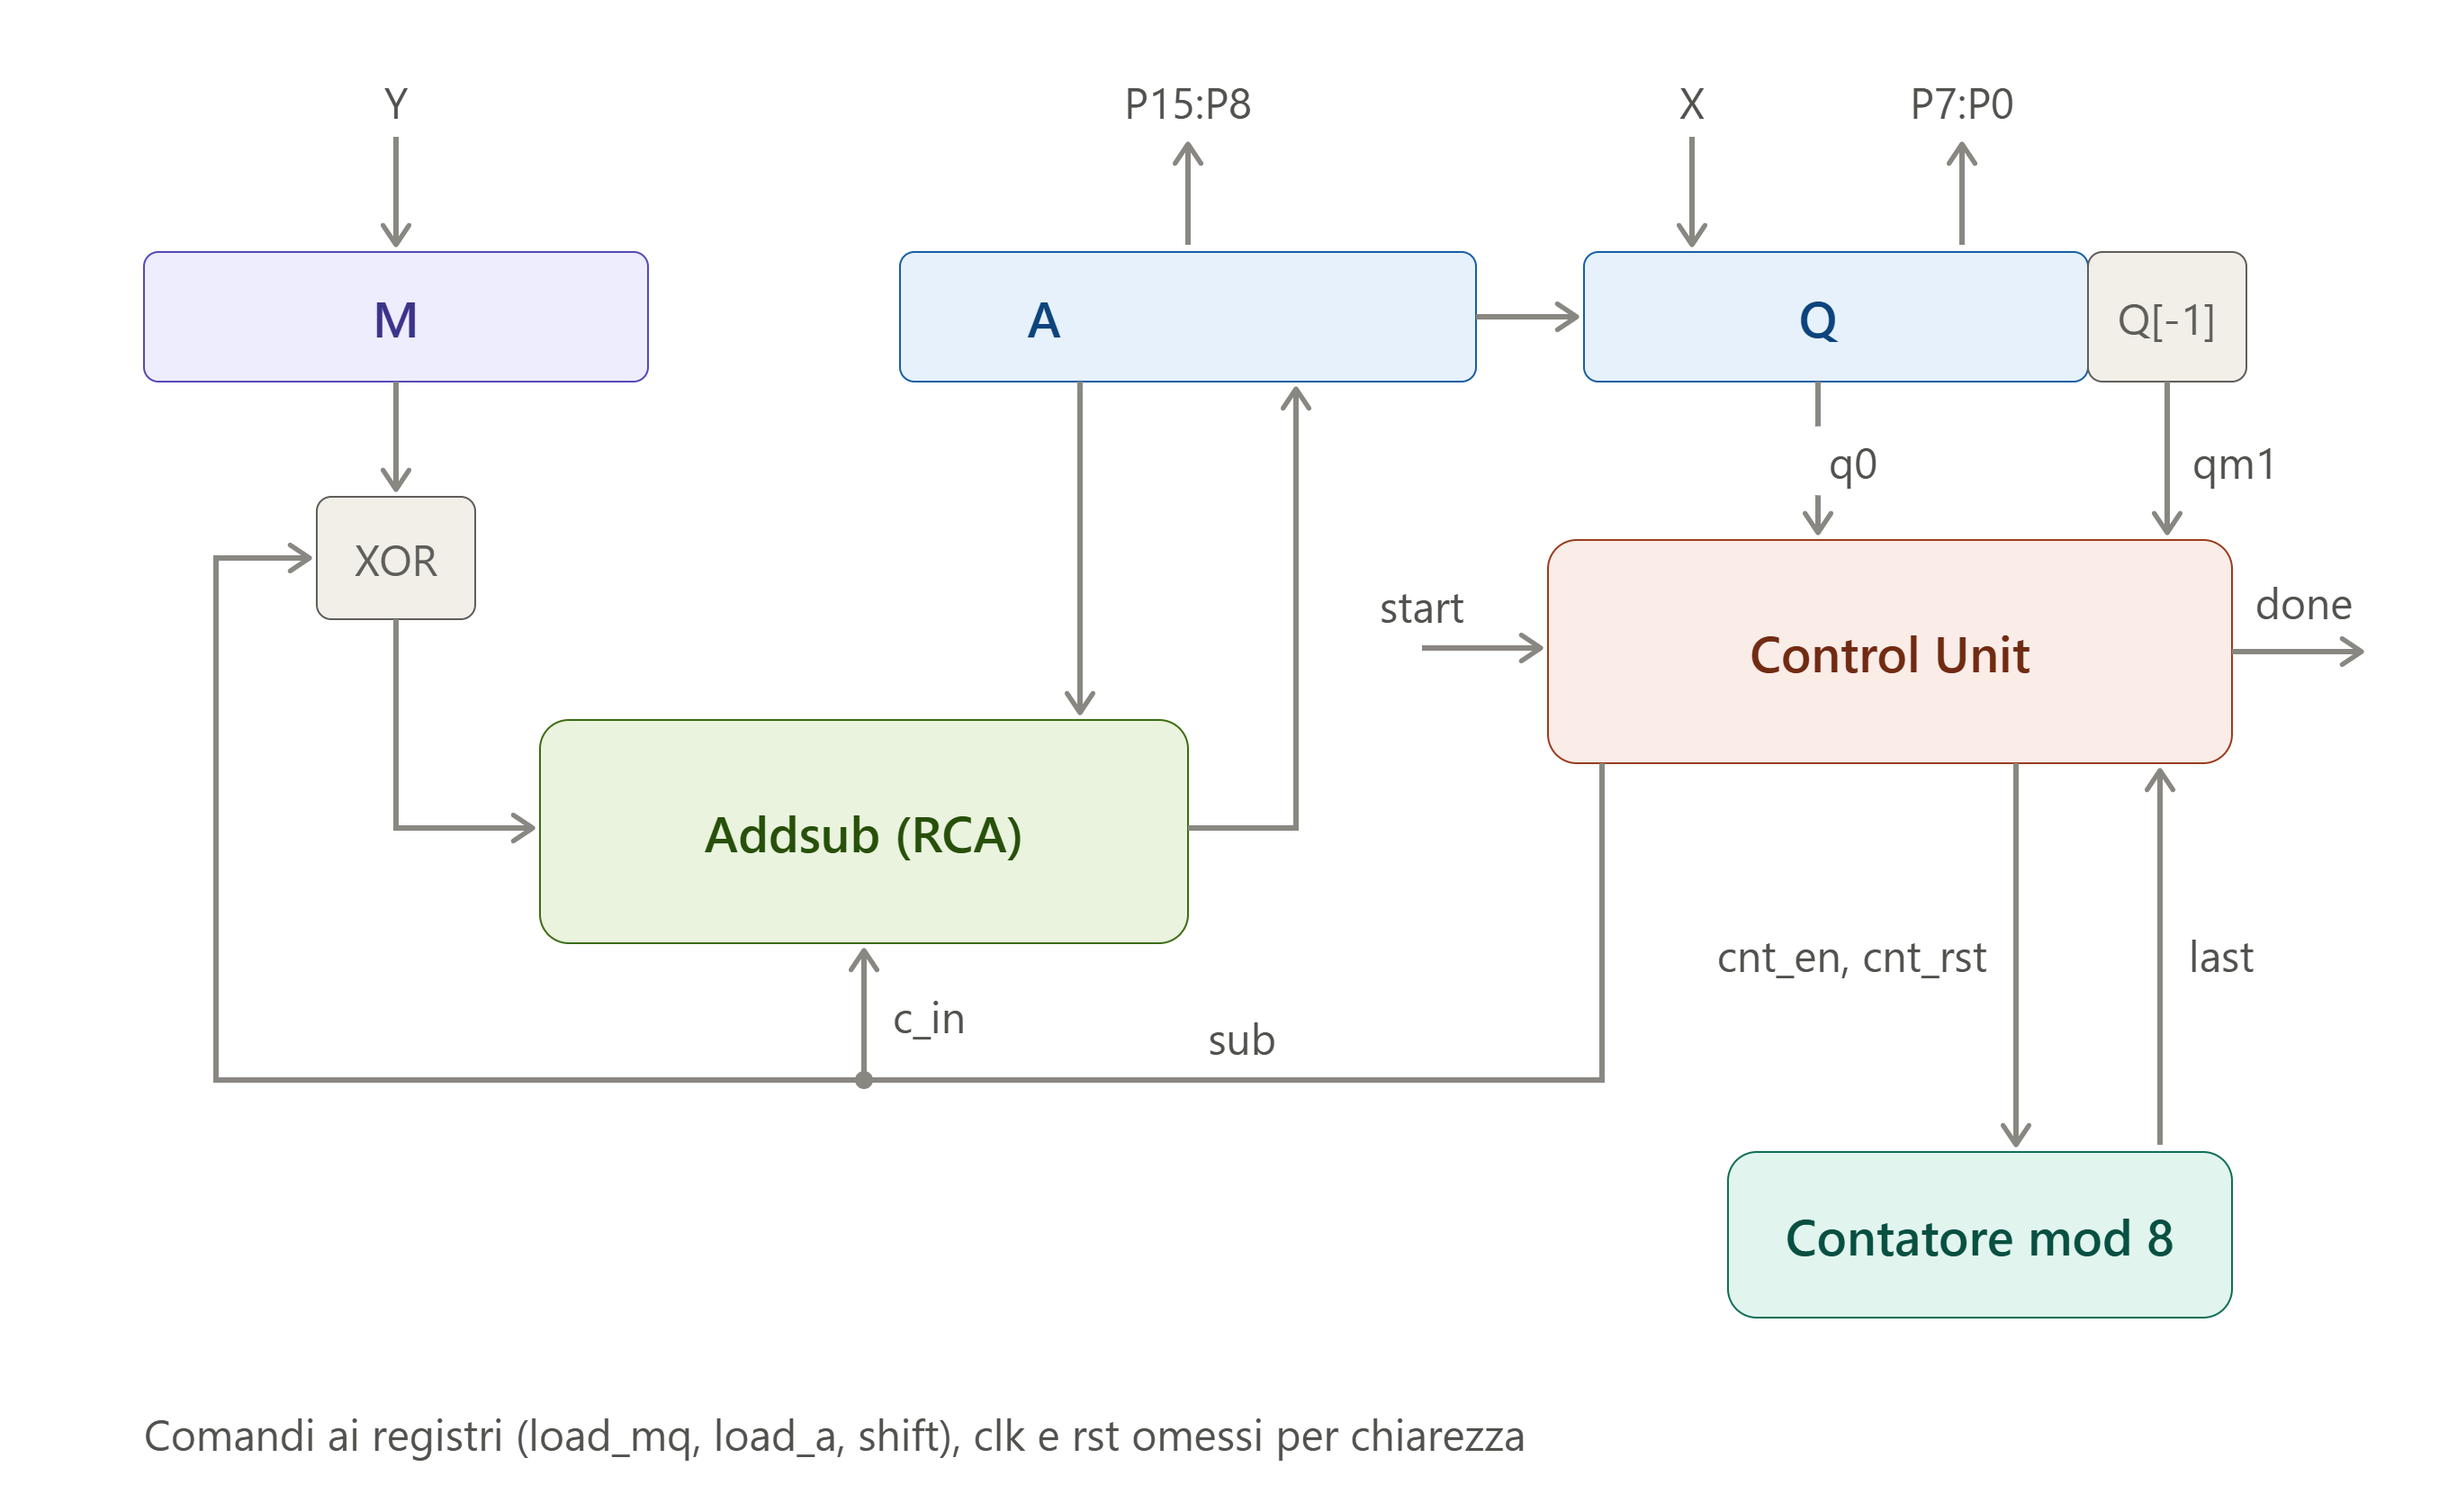
\includegraphics[width=0.7\linewidth]{figure/esercizio7-1/schema}
  \caption{Architettura del moltiplicatore di Booth}
  \label{fig:esercizio7-1:schema}
\end{figure}

Il sommatore riceve \texttt{A} e \texttt{M}, quest'ultimo attraverso uno strato di XOR pilotato da \texttt{sub}. Lo stesso segnale è anche il riporto in ingresso: con \texttt{sub} a \texttt{'1'} si ottiene $A - M$, con \texttt{sub} a \texttt{'0'} si ottiene $A + M$. Il risultato viene ricaricato in \texttt{A}, mentre il prodotto a 16 bit è la concatenazione di \texttt{A} e \texttt{Q}.

A differenza della soluzione proposta nel documento di riferimento, registri e shift register non sono istanziati come componenti separati: \texttt{M}, \texttt{A}, \texttt{Q} e \texttt{Q[-1]} sono segnali aggiornati da un unico process della parte operativa. Il contatore è invece quello parametrico già utilizzato altrove (\texttt{counter\_mod}), non uno dedicato.

\implementazione

Si riportano di seguito i componenti in ordine bottom-up, a partire dal \texttt{full\_adder}: tre ingressi (\texttt{a}, \texttt{b}, \texttt{c\_in}), due uscite (\texttt{s}, \texttt{c\_out}) e architettura dataflow con assegnazioni concorrenti.

\vhdlfile{esercizio7-1/full_adder.vhd}{Implementazione Full Adder}{lst:esercizio7-1:full-adder}

Il componente \texttt{rca} realizza il ripple carry adder a $N$ bit (generic \texttt{N}, di default 8) con architettura structural: un \texttt{for generate} istanzia $N$ full adder collegati tramite il vettore di riporti interno \texttt{c}. Oltre alla somma e al riporto in uscita c'è \texttt{ovf}, ottenuto come XOR tra gli ultimi due riporti.

\vhdlfile{esercizio7-1/rca.vhd}{Implementazione Ripple Carry Adder}{lst:esercizio7-1:rca}

L'entità \texttt{add\_sub} ha gli stessi generic e le stesse porte dell'\texttt{rca}, ma \texttt{c\_in} fa da selettore: un ciclo \texttt{for generate} calcola lo XOR tra ogni bit di \texttt{b} e \texttt{c\_in}, e il vettore ottenuto alimenta il ripple carry adder. Con \texttt{c\_in} a \texttt{'1'} l'operando è complementato e il riporto iniziale aggiunge uno: è la sottrazione in complemento a due.

\vhdlfile{esercizio7-1/add_sub.vhd}{Implementazione Addizionatore/Sottrattore}{lst:esercizio7-1:add-sub}

Il contatore modulo $M$ che conta gli otto passi è quello presentato nel Listato~\ref{lst:esercizio5-1:counter-mod} e non viene ripetuto.

La parte operativa \texttt{booth\_po} riceve \texttt{x} (moltiplicatore) e \texttt{y} (moltiplicando) e restituisce il prodotto \texttt{p} a 16 bit, insieme ai segnali di stato \texttt{q0}, \texttt{qm1} e \texttt{last}; i comandi provengono dalla CU. L'architettura, denominata \texttt{mixed}, unisce due istanze (\texttt{add\_sub} con \texttt{N} pari a 8 e \texttt{counter\_mod} con \texttt{M} pari a 8 e \texttt{W} pari a 3) a un process sincrono, \texttt{registri}, sensibile al solo \texttt{clk}. Le condizioni hanno priorità decrescente: \texttt{rst} azzera tutti i registri; \texttt{load\_mq} carica \texttt{M} con \texttt{y}, \texttt{Q} con \texttt{x} e azzera \texttt{A} e \texttt{Q[-1]}; \texttt{load\_a} memorizza in \texttt{A} l'uscita del sommatore; \texttt{shift} esegue lo shift a destra della coppia \texttt{A}, \texttt{Q}, replicando il bit di segno di \texttt{A} e passando il bit uscente di \texttt{Q} in \texttt{Q[-1]}. Il contatore riceve \texttt{load} fisso a \texttt{'0'} e usa come reset il segnale \texttt{cnt\_rst}; la sua uscita \texttt{tc} è il segnale \texttt{last}.

\vhdlfile{esercizio7-1/booth_po.vhd}{Implementazione parte operativa del moltiplicatore di Booth}{lst:esercizio7-1:booth-po}

L'unità di controllo \texttt{booth\_cu} è una FSM a cinque stati (\texttt{S\_IDLE}, \texttt{S\_INIT}, \texttt{S\_ADD}, \texttt{S\_SHIFT}, \texttt{S\_DONE}) descritta con due process: \texttt{f\_controllo}, combinatorio, calcola stato prossimo e uscite (assegnate a valori di default all'inizio del process); \texttt{mem\_stato}, sincrono con reset sincrono, aggiorna lo stato. In \texttt{S\_IDLE} si attende \texttt{start}; in \texttt{S\_INIT} vengono attivati \texttt{load\_mq} e \texttt{cnt\_rst}; in \texttt{S\_ADD} si esamina la coppia \texttt{q0}, \texttt{qm1} e si attiva \texttt{load\_a}, insieme a \texttt{sub} nel caso $10_2$, mentre per $00_2$ e $11_2$ non viene fatto nulla; in \texttt{S\_SHIFT} si attivano \texttt{shift} e \texttt{cnt\_en}, e si torna in \texttt{S\_ADD} finché \texttt{last} non vale \texttt{'1'}. Infine, in \texttt{S\_DONE} si alza \texttt{done}, e si torna in \texttt{S\_IDLE} solo quando \texttt{start} è riportato a \texttt{'0'}.

\vhdlfile{esercizio7-1/booth_cu.vhd}{Implementazione unità di controllo del moltiplicatore di Booth}{lst:esercizio7-1:booth-cu}

Il top module \texttt{booth} ha come ingressi \texttt{clk}, \texttt{rst}, \texttt{start}, \texttt{x} e \texttt{y} (8 bit) e come uscite \texttt{p} (16 bit) e \texttt{done}. L'architettura è structural: istanzia con port mapping \texttt{booth\_po} e \texttt{booth\_cu} e li collega tramite i segnali di comando e di stato.

\vhdlfile{esercizio7-1/booth.vhd}{Implementazione top module del moltiplicatore di Booth}{lst:esercizio7-1:booth}

\simulazione

Il testbench \texttt{booth\_tb} ha un'entità priva di porte e istanzia il top module come \texttt{dut}. Ha due process: \texttt{clk\_proc}, che genera un clock con periodo di 10 ns, e \texttt{stim}, che mantiene il reset per due periodi, assegna gli ingressi, alza \texttt{start} e attende \texttt{done} con \texttt{wait until}. A quel punto un \texttt{assert} confronta \texttt{p} con il valore atteso e un \texttt{report} stampa il prodotto calcolato; infine \texttt{start} torna a \texttt{'0'} e un \texttt{wait;} chiude il process. La soluzione proposta verifica più coppie di operandi, mentre questo testbench prova un solo caso.

\vhdlfile{esercizio7-1/booth_tb.vhd}{Testbench del moltiplicatore di Booth}{lst:esercizio7-1:booth-tb}

Il risultato della simulazione è in figura~\ref{fig:esercizio7-1:simulazione}.

\begin{figure}[H]
  \centering
  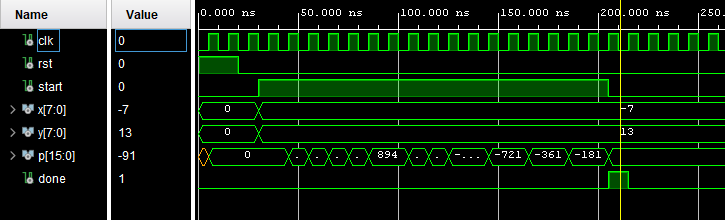
\includegraphics[width=0.95\linewidth]{figure/esercizio7-1/simulazione}
  \caption{Simulazione del moltiplicatore di Booth}
  \label{fig:esercizio7-1:simulazione}
\end{figure}

Il caso simulato è $(-7) \cdot 13$: \texttt{x} vale $-7_{10}$ (0xF9, $11111001_2$) e \texttt{y} vale $13_{10}$ (0x0D, $00001101_2$). Dopo il rilascio del reset, \texttt{start} passa a \texttt{'1'} e \texttt{p} attraversa i prodotti parziali durante gli otto passi (nella forma d'onda compaiono, tra gli altri, i valori $-721_{10}$, $-361_{10}$ e $-181_{10}$). A circa 200 ns \texttt{done} si porta a \texttt{'1'} e \texttt{p} vale $-91_{10}$, coincidente con il valore atteso.

\begin{risultato}
Con \texttt{x} $= -7$ e \texttt{y} $= 13$, all'attivazione di \texttt{done} l'uscita \texttt{p} vale $-91$, come previsto dall'\texttt{assert} del testbench.
\end{risultato}

\esSezione{Moltiplicatore di Booth su board}\label{sec:esercizio7-2}

\begin{traccia}
Sintetizzare il moltiplicatore implementato al punto~\ref{sec:esercizio7-1} su FPGA e testarlo mediante l'utilizzo dei dispositivi di input/output (switch, bottoni, led, display) presenti sulla board di sviluppo in dotazione. La modalità di utilizzo degli stessi è a completa discrezione degli studenti.
\end{traccia}

\progetto

Il moltiplicatore di Booth dell'esercizio~\ref{sec:esercizio7-1} viene istanziato così com'è in un nuovo top module, che si limita a collegarne le porte ai dispositivi della board. Non sono stati aggiunti componenti: il sistema è composto dalle sole entità già presentate (\texttt{booth}, \texttt{booth\_po}, \texttt{booth\_cu}, \texttt{add\_sub}, \texttt{rca}, \texttt{full\_adder}, \texttt{counter\_mod}), richiamate nei listati~\ref{lst:esercizio7-1:booth}, \ref{lst:esercizio7-1:booth-po}, \ref{lst:esercizio7-1:booth-cu}, \ref{lst:esercizio7-1:add-sub}, \ref{lst:esercizio7-1:rca}, \ref{lst:esercizio7-1:full-adder} e~\ref{lst:esercizio5-1:counter-mod}.

L'assegnazione dei dispositivi è la seguente:

\begin{itemize}
  \item i sedici switch forniscono gli operandi: \texttt{SW(15 downto 8)} per il moltiplicando \texttt{x} e \texttt{SW(7 downto 0)} per il moltiplicatore \texttt{y};
  \item il pulsante centrale \texttt{BTNC} è il segnale \texttt{start};
  \item il pulsante inferiore \texttt{BTND} è il segnale \texttt{rst};
  \item i sedici LED \texttt{LED(15 downto 0)} mostrano in binario il prodotto \texttt{p};
  \item il LED verde \texttt{LED16\_G} segnala il termine dell'operazione tramite \texttt{done}.
\end{itemize}

Si è scelto di non inserire debouncer né circuiti di visualizzazione su display: l'unità di controllo evolve a ogni fronte di salita del clock a \SI{100}{MHz} e sfrutta lo stato \texttt{S\_DONE}, nel quale resta finché \texttt{start} non torna a \texttt{'0'}. Il prodotto, in complemento a due, resta quindi stabile sui LED fino alla pressione successiva.

\implementazione

Il top module \texttt{booth\_tl} ha come porte il clock \texttt{CLK100MHZ}, il vettore \texttt{SW} a 16 bit, i pulsanti \texttt{BTNC} e \texttt{BTND}, il vettore \texttt{LED} a 16 bit e l'uscita \texttt{LED16\_G}. L'architettura \texttt{structural} contiene un'unica istanza, \texttt{Mbooth}, del componente \texttt{booth} (architettura \texttt{structural}), collegata con un port mapping diretto alle porte del top module.

\vhdlfile{esercizio7-2/booth_tl.vhd}{Implementazione del top module per la board}{lst:esercizio7-2:booth-tl}

Non è stato scritto un testbench specifico per questo top module, che non contiene logica propria.

\sintesiboard

Sulla scheda si impostano gli operandi con gli switch e si preme \texttt{BTNC}: la moltiplicazione parte e, alla conclusione degli otto passi, si accende \texttt{LED16\_G} mentre i LED \texttt{LED(15 downto 0)} riportano il prodotto a 16 bit. Rilasciando \texttt{BTNC} l'unità di controllo torna nello stato di attesa e una nuova operazione può essere avviata; \texttt{BTND} riporta il sistema alla condizione iniziale. % TODO: esiti della prova su board (foto/valori osservati) non disponibili

Nel file dei constraint sono state decommentate le seguenti righe.

\xdcfile{esercizio7-2/vincoli.xdc}{Constraint}{lst:esercizio7-2:vincoli}
\begin{figure}[H]
  \centering
  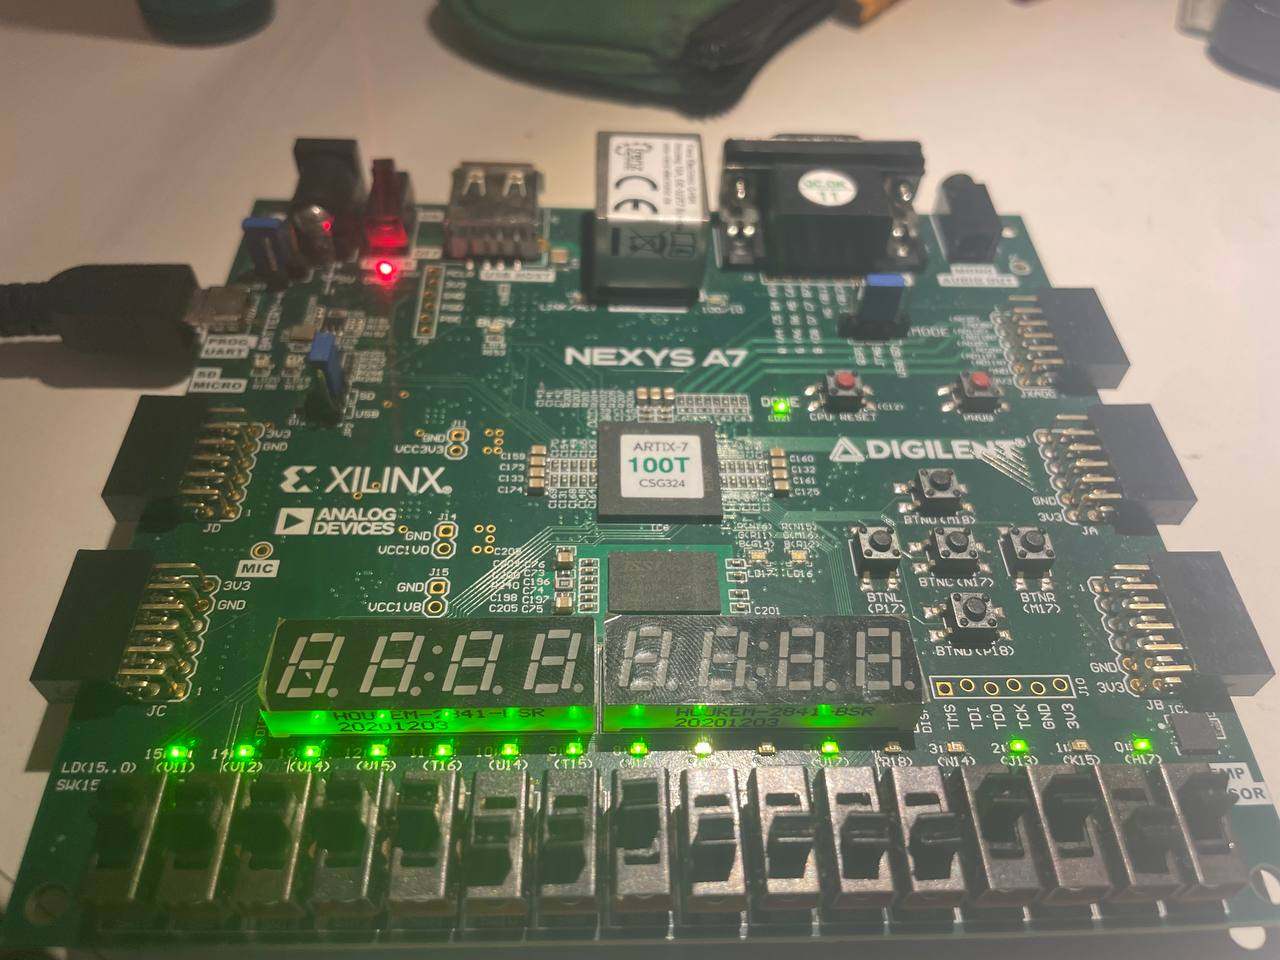
\includegraphics[width=\linewidth]{figure/esercizio7-2/irl.jpg}
  \caption{Realizzazione del moltiplicatore di Booth}
  \label{fig:esercizio7-2:booth}
\end{figure}

\esCapitolo{Comunicazione con handshaking}\label{cap:handshaking}
\esSezione{Comunicazione con handshaking}\label{sec:esercizio8-1}

\begin{traccia}
Progettare, implementare in VHDL e testare mediante simulazione un sistema formato da due nodi, A e B, che comunicano con un protocollo di handshaking. Ciascun nodo dispone di una memoria interna con $N$ stringhe di $M$ bit, indicate rispettivamente con $X(i)$ e $Y(i)$, per $i = 0, \dots, N-1$. Il nodo A trasmette a B ogni stringa $X(i)$; B, ricevutala, calcola $S(i) = X(i) + Y(i)$ e memorizza la somma nella propria memoria. La somma può essere descritta in modo comportamentale, mentre in entrambi i nodi deve essere presente un componente contatore che scandisce le stringhe e determina la fine della comunicazione.
\end{traccia}

\progetto

Il sistema è composto da due entità, \texttt{system\_A} e \texttt{system\_B}, collegate dai segnali \texttt{req}, \texttt{ack} e \texttt{data}. Il nodo A contiene una Control Unit, una ROM con le stringhe $X(i)$ e un contatore che ne scandisce gli indirizzi. Il nodo B contiene una Control Unit, un registro che cattura il dato ricevuto, un adder, una memoria con le stringhe $Y(i)$ (nella quale viene scritta anche la somma) e un contatore degli indirizzi. I due nodi lavorano con clock indipendenti, quindi la sincronizzazione è affidata al solo handshaking. La figura~\ref{fig:esercizio8-1:architettura} illustra l'architettura complessiva, con il clock omesso per chiarezza.

\begin{figure}[H]
  \centering
  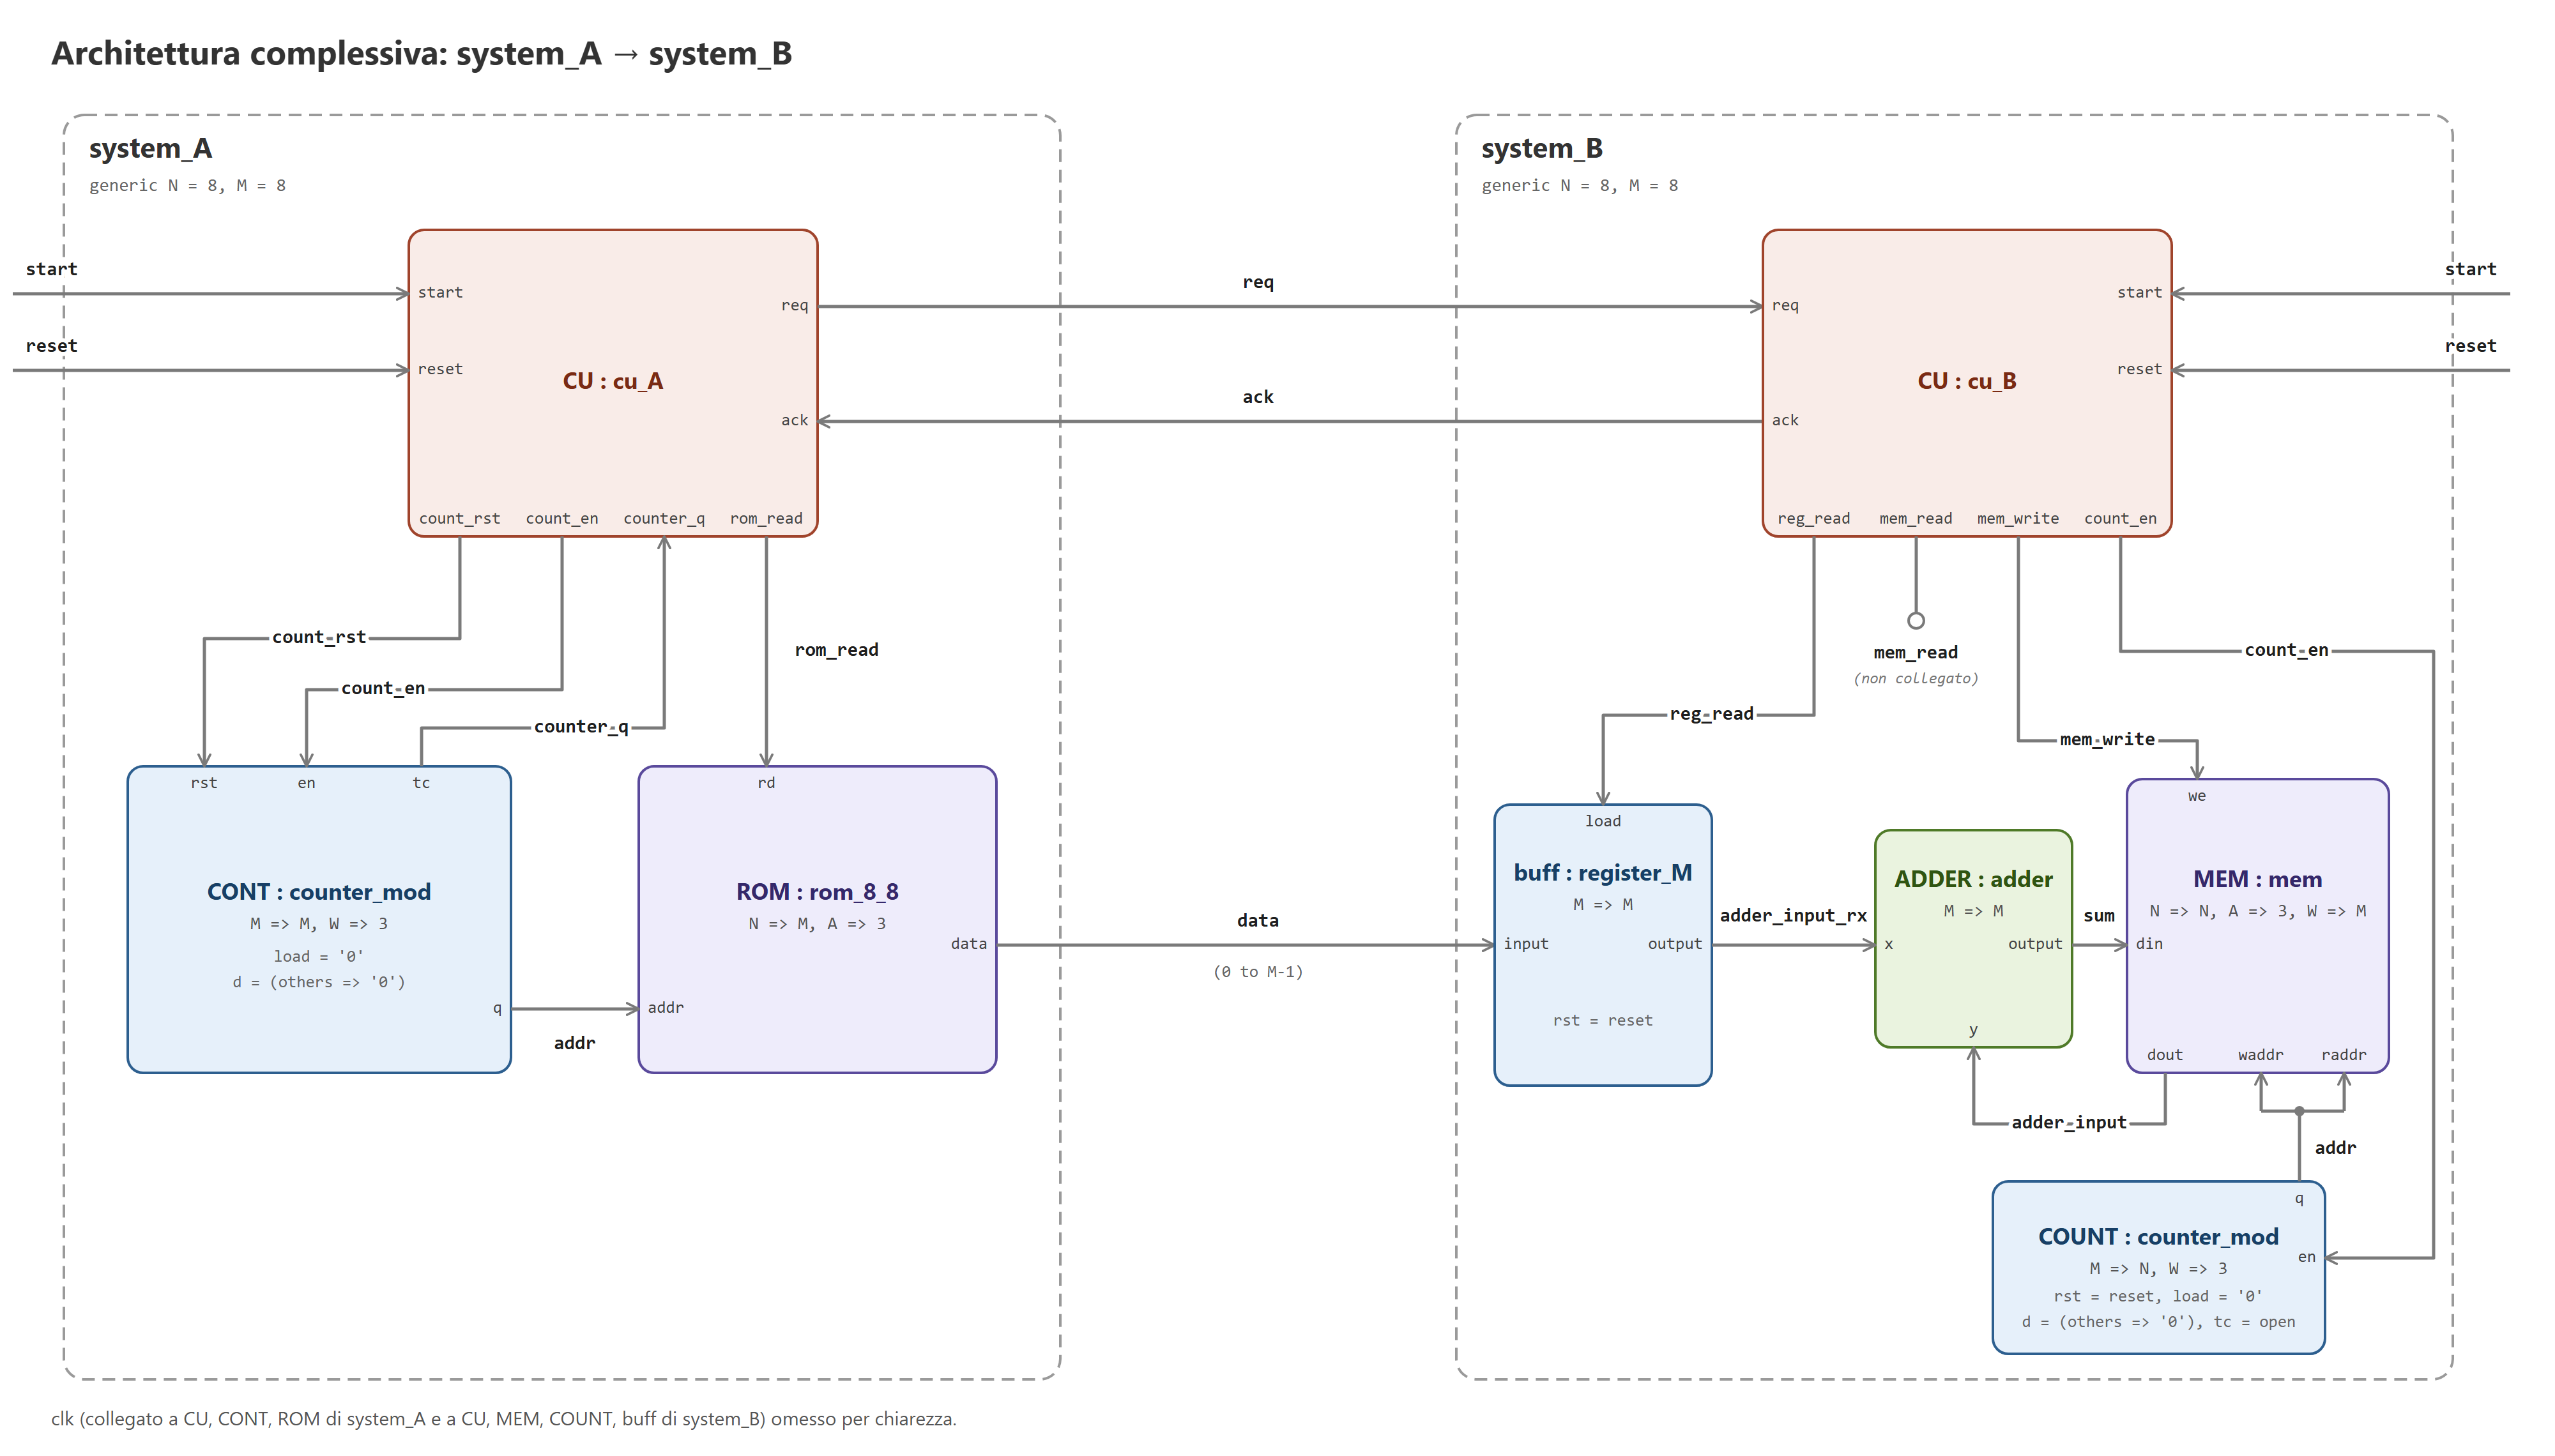
\includegraphics[width=\linewidth]{figure/esercizio8-1/architettura}
  \caption{Architettura del sistema di handshaking}
  \label{fig:esercizio8-1:architettura}
\end{figure}

Il protocollo è a quattro fasi. A porta \texttt{req} a \texttt{'1'} dopo aver letto il dato dalla ROM e attende \texttt{ack} a \texttt{'1'}; B, visto \texttt{req}, cattura il dato nel registro e alza \texttt{ack}; A abbassa \texttt{req}; B, rilevato \texttt{req} a \texttt{'0'}, scrive la somma in memoria, incrementa il contatore e abbassa \texttt{ack}. Solo a questo punto A passa alla stringa successiva. Le unità di controllo sono descritte dalle FSM nelle figure~\ref{fig:esercizio8-1:fsm-a} e~\ref{fig:esercizio8-1:fsm-b}.

\begin{figure}[H]
  \centering
  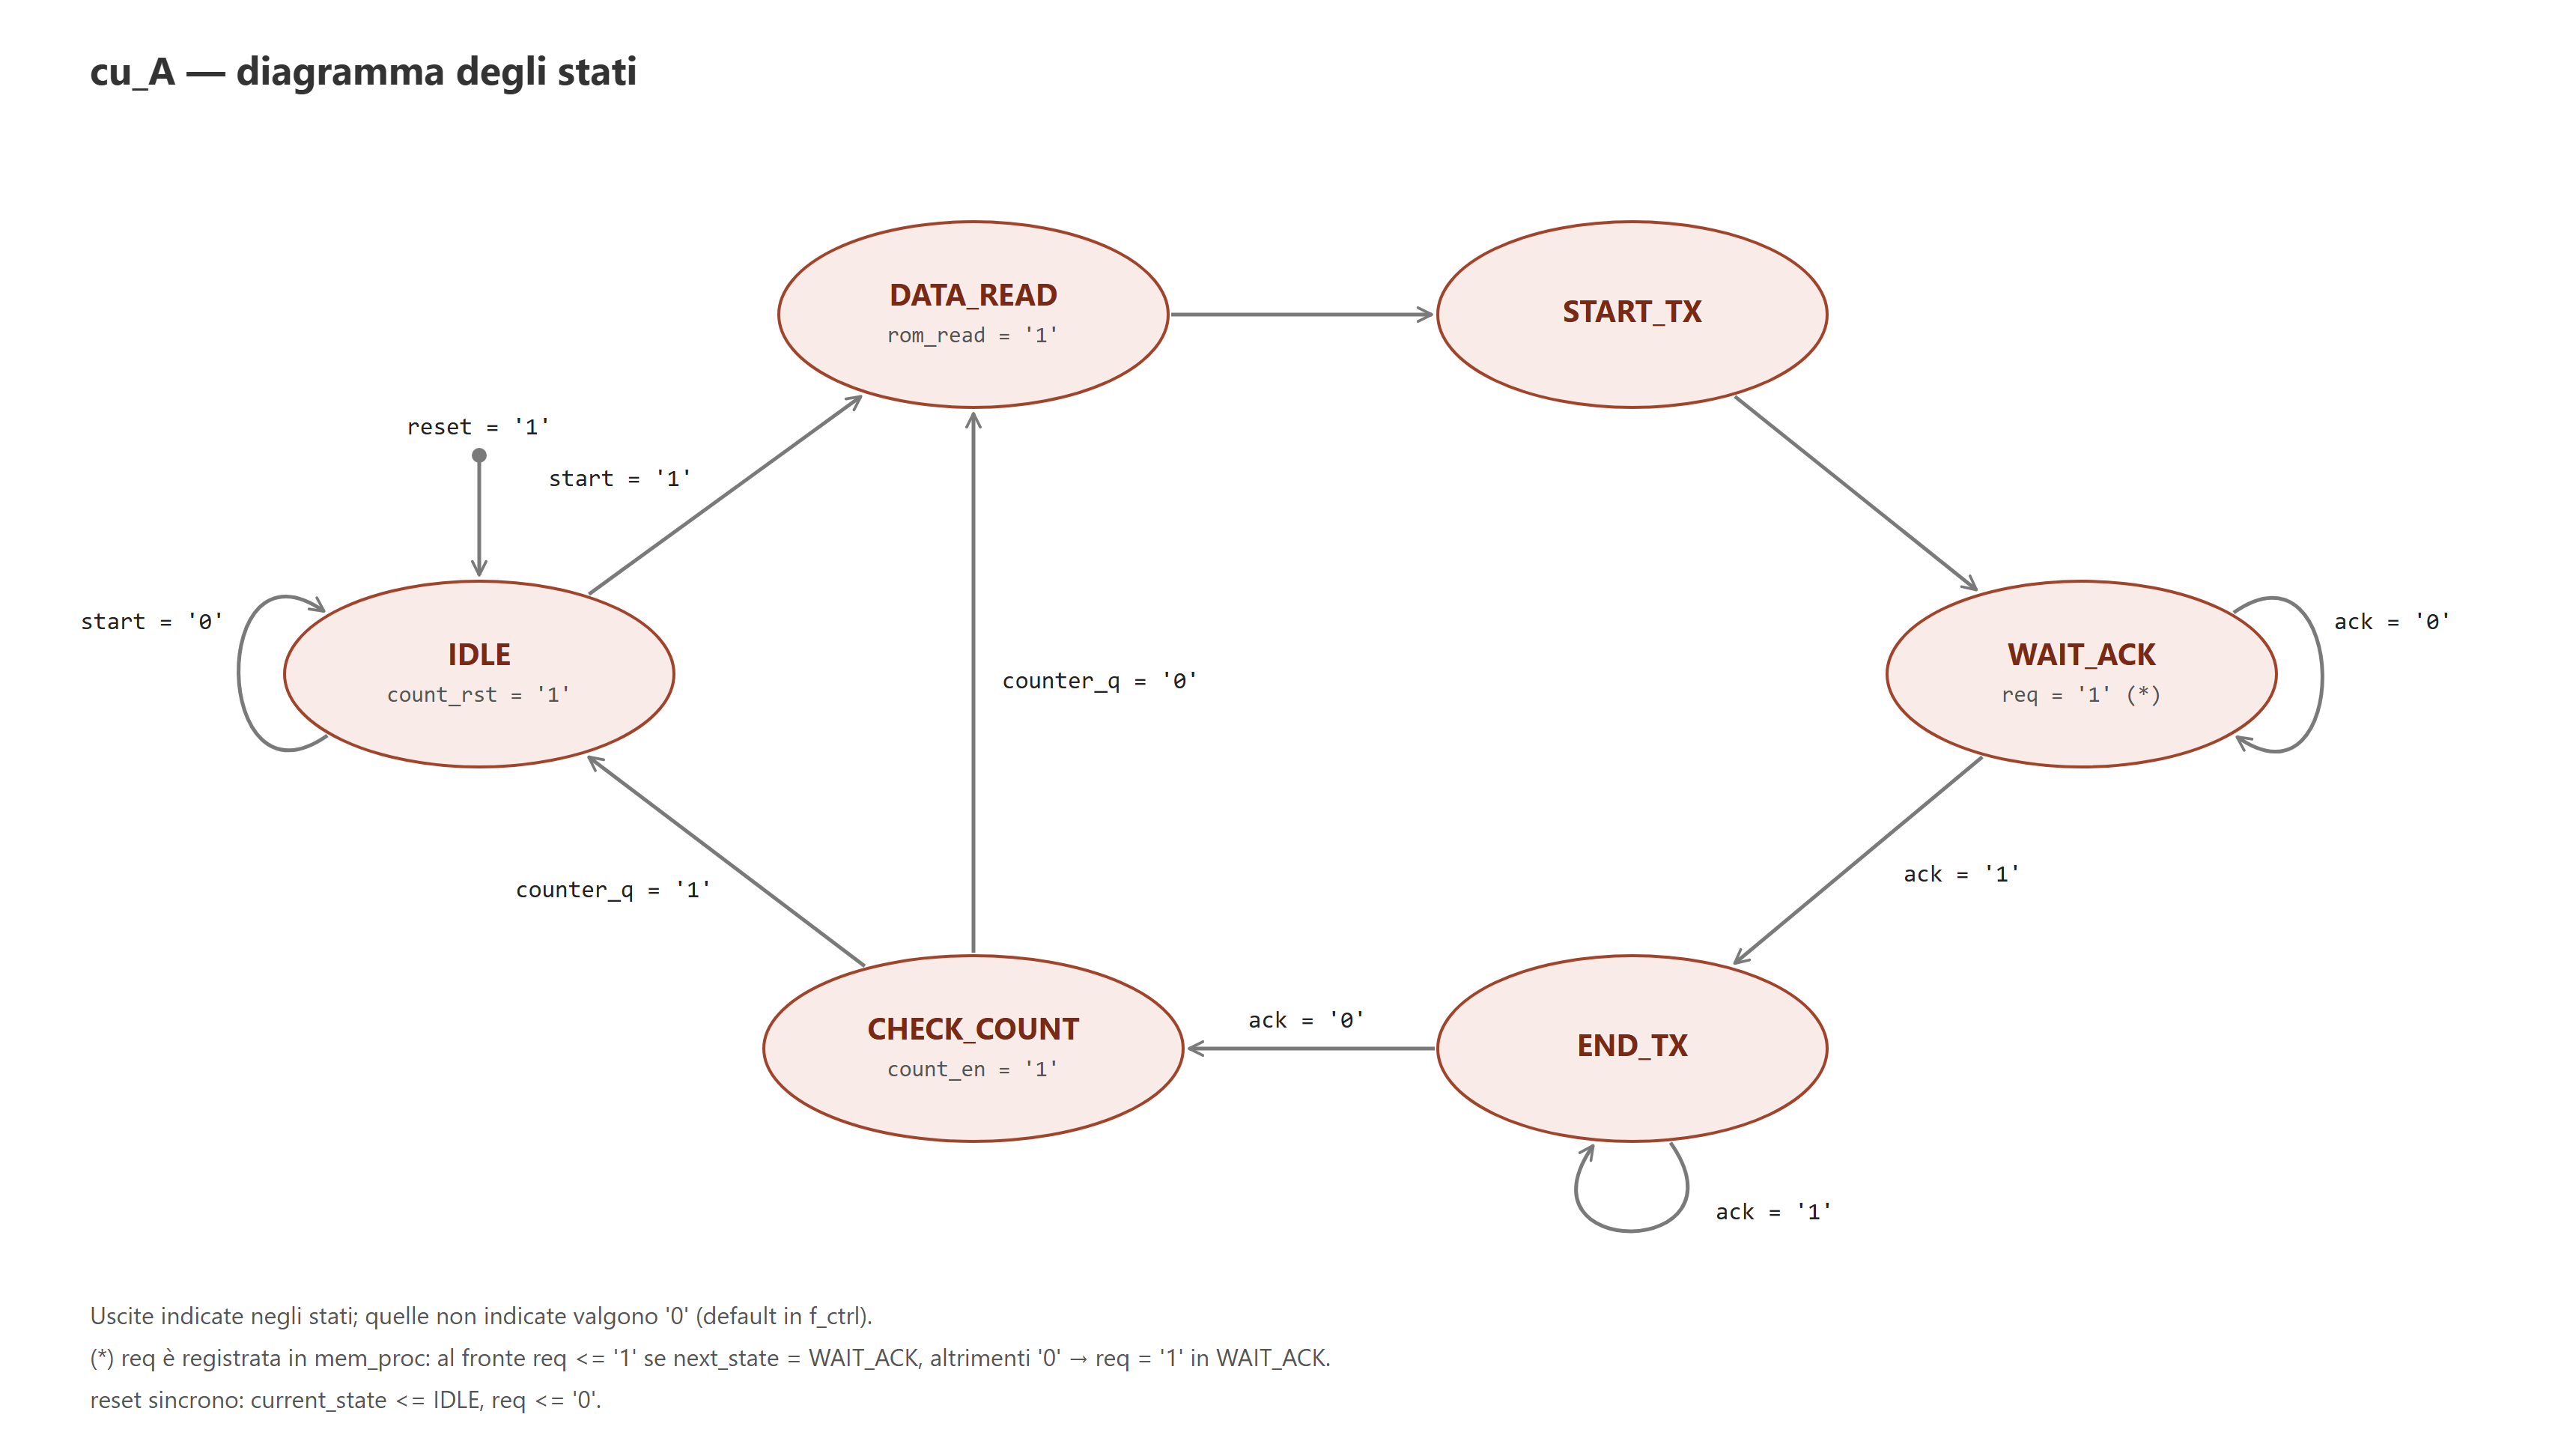
\includegraphics[width=0.8\linewidth]{figure/esercizio8-1/fsm-a}
  \caption{FSM dell'unità A}
  \label{fig:esercizio8-1:fsm-a}
\end{figure}

\begin{figure}[H]
  \centering
  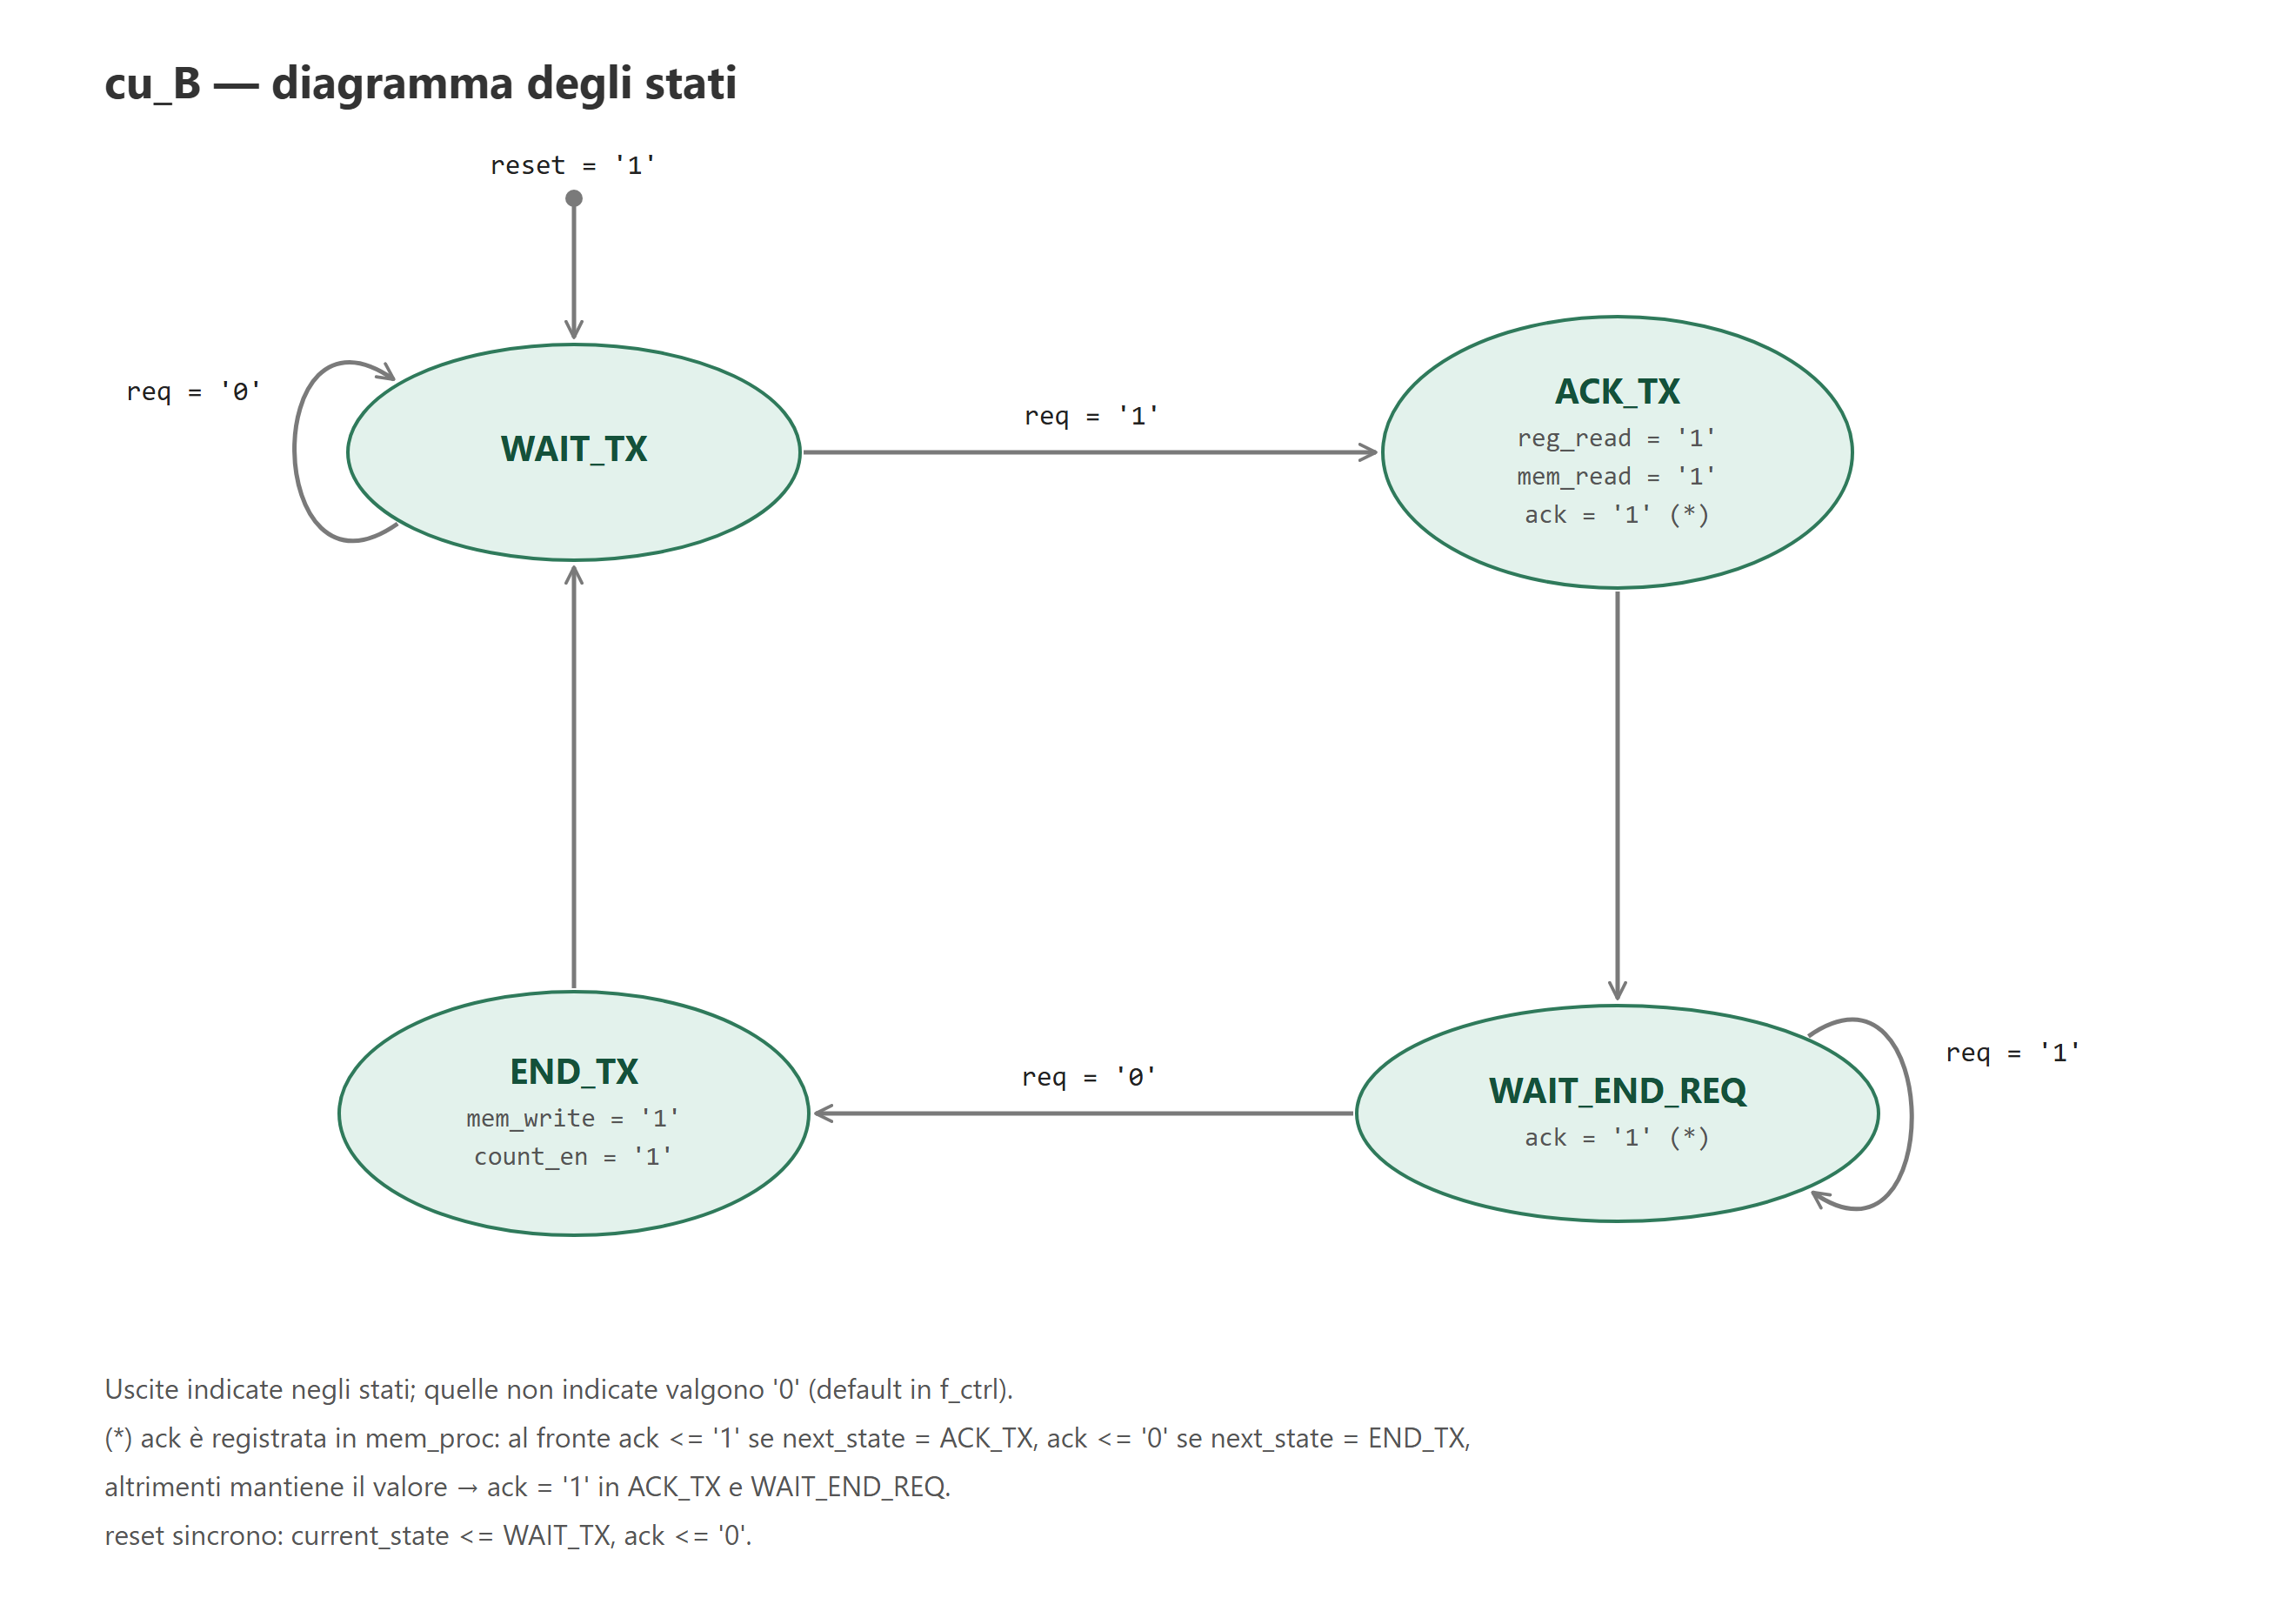
\includegraphics[width=0.6\linewidth]{figure/esercizio8-1/fsm-b}
  \caption{FSM dell'unità B}
  \label{fig:esercizio8-1:fsm-b}
\end{figure}

Nelle figure le uscite non indicate in uno stato valgono \texttt{'0'}; \texttt{req} e \texttt{ack} sono uscite registrate, aggiornate al fronte di clock in funzione dello stato successivo (segnalate con un asterisco). L'FSM di A ha sei stati (\texttt{IDLE}, \texttt{DATA\_READ}, \texttt{START\_TX}, \texttt{WAIT\_ACK}, \texttt{END\_TX}, \texttt{CHECK\_COUNT}) e quella di B quattro (\texttt{WAIT\_TX}, \texttt{ACK\_TX}, \texttt{WAIT\_END\_REQ}, \texttt{END\_TX}).

\begin{osservazione}
Rispetto alla soluzione proposta, l'implementazione differisce nei seguenti punti:
\begin{itemize}
  \item le unità di controllo sono \texttt{cu\_A} e \texttt{cu\_B}, con porte \texttt{clk}, \texttt{count\_en} e \texttt{count\_rst} (invece di \texttt{clock}, \texttt{counter\_enable} e \texttt{counter\_reset});
  \item la FSM di A include \texttt{WAIT\_ACK} (non \texttt{DATA\_WAIT}) e non usa one-hot esplicita;
  \item le FSM sono descritte con due process distinti (combinatorio e sequenziale);
  \item la ROM del nodo A è \texttt{rom\_8\_8} con contenuto fisso;
  \item memoria e contatore sono componenti comuni;
  \item \texttt{cu\_B} riceve \texttt{start} inutilizzato e l'uscita \texttt{mem\_read} non è collegata.
\end{itemize}
\end{osservazione}

\implementazione

Il contatore \texttt{counter\_mod} (listato~\ref{lst:esercizio5-1:counter-mod}) e la memoria \texttt{mem} (listato~\ref{lst:esercizio6-1:mem}) sono già stati presentati e vengono istanziati senza modifiche. Il componente \texttt{rom} (listato~\ref{lst:esercizio6-1:rom}), pur incluso nel progetto Vivado, non è istanziato in questo esercizio: il nodo A usa la ROM dedicata \texttt{rom\_8\_8}. Vediamo ora i componenti propri dell'esercizio, partendo dal nodo B.

Il registro \texttt{register\_M} ha larghezza $M$ (generic, default 8) e porte \texttt{clk}, \texttt{rst}, \texttt{load}, \texttt{input} e \texttt{output}. Un process sincrono azzera il dato con \texttt{rst} attivo e lo carica al fronte di salita quando \texttt{load} è \texttt{'1'}.

\vhdlfile{esercizio8-1/register_m.vhd}{Implementazione del registro}{lst:esercizio8-1:register-m}

L'\texttt{adder} ha architettura dataflow e somma i due ingressi \texttt{x} e \texttt{y} di $M$ bit, interpretati come \texttt{unsigned}. L'uscita \texttt{output} ha gli stessi $M$ bit, quindi il riporto viene scartato.

\vhdlfile{esercizio8-1/adder.vhd}{Implementazione dell'adder}{lst:esercizio8-1:adder}

La \texttt{rom\_8\_8} ha generic \texttt{N} (locazioni) e \texttt{A} (bit di indirizzo) e memorizza in una costante otto byte: \texttt{x"00"}, \texttt{x"FF"}, \texttt{x"01"}, \texttt{x"80"}, \texttt{x"0F"}, \texttt{x"F0"}, \texttt{x"AA"}, \texttt{x"55"}. Un'\texttt{assert} verifica che \texttt{N} sia indirizzabile su \texttt{A} bit; la lettura è sincrona, controllata da \texttt{rd}.

\vhdlfile{esercizio8-1/rom_8_8.vhd}{Implementazione della ROM 8x8}{lst:esercizio8-1:rom-8-8}

L'unità di controllo \texttt{cu\_A} è descritta con due process. Il process \texttt{f\_ctrl}, combinatorio, calcola stato successivo e uscite (\texttt{count\_rst} in \texttt{IDLE}, \texttt{rom\_read} in \texttt{DATA\_READ}, \texttt{count\_en} in \texttt{CHECK\_COUNT}); il process \texttt{mem\_proc}, sincrono, aggiorna lo stato e registra \texttt{req}, che vale \texttt{'1'} quando lo stato successivo è \texttt{WAIT\_ACK}. In \texttt{CHECK\_COUNT} l'ingresso \texttt{counter\_q} decide se tornare a \texttt{IDLE} (ultima stringa) o proseguire con \texttt{DATA\_READ}.

\vhdlfile{esercizio8-1/cu_a.vhd}{Implementazione della CU A}{lst:esercizio8-1:cu-a}

L'unità \texttt{cu\_B} ha la stessa struttura a due process: in \texttt{ACK\_TX} attiva \texttt{reg\_read} e \texttt{mem\_read}; in \texttt{END\_TX} attiva \texttt{mem\_write} e \texttt{count\_en}. L'uscita \texttt{ack}, registrata, sale quando lo stato successivo è \texttt{ACK\_TX}, scende quando è \texttt{END\_TX} e negli altri casi mantiene il valore.

\vhdlfile{esercizio8-1/cu_b.vhd}{Implementazione della CU B}{lst:esercizio8-1:cu-b}

Il top module del nodo A, \texttt{system\_A}, ha generic \texttt{N} e \texttt{M} e istanzia tramite port mapping la \texttt{cu\_A}, un \texttt{counter\_mod} (con \texttt{W} pari a 3, reset da \texttt{count\_rst}, abilitazione da \texttt{count\_en} e riporto \texttt{tc} verso \texttt{counter\_q}) e la \texttt{rom\_8\_8}, indirizzata dall'uscita del contatore.

\vhdlfile{esercizio8-1/system_a.vhd}{Implementazione del sistema A}{lst:esercizio8-1:system-a}

Il top module del nodo B, \texttt{system\_B}, istanzia \texttt{cu\_B}, \texttt{mem}, un \texttt{counter\_mod}, l'\texttt{adder} e il registro \texttt{buff}. Il registro cattura il dato ricevuto quando \texttt{reg\_read} è alto; l'adder somma il contenuto del registro (\texttt{adder\_input\_rx}) al valore letto dalla memoria all'indirizzo corrente (\texttt{adder\_input}); il risultato \texttt{sum} viene scritto nella stessa locazione quando \texttt{mem\_write} è alto. Lo stesso indirizzo pilota lettura e scrittura, e l'uscita di terminal count del contatore non è utilizzata.

\vhdlfile{esercizio8-1/system_b.vhd}{Implementazione del sistema B}{lst:esercizio8-1:system-b}

\simulazione

Il testbench \texttt{handshaking\_tb} ha entità senza porte e istanzia \texttt{system\_A} (\texttt{sysA}) e \texttt{system\_B} (\texttt{sysB}) con $N = M = 8$, collegando \texttt{req}, \texttt{ack} e \texttt{data}. Due process, \texttt{clockA} e \texttt{clockB}, generano clock con periodo di \SI{10}{ns} e \SI{11}{ns}, per verificare il funzionamento con clock diversi. Il process \texttt{stim\_proc} attende \SI{100}{ns}, impone \texttt{rst} per \SI{10}{ns}, attende altri \SI{10}{ns}, alza \texttt{start} per \SI{10}{ns} e termina con \texttt{wait;}. Non sono presenti \texttt{assert}: il controllo avviene per ispezione delle forme d'onda.

\vhdlfile{esercizio8-1/handshaking_tb.vhd}{Testbench dell'handshaking}{lst:esercizio8-1:handshaking-tb}

Il risultato della simulazione è riportato in figura~\ref{fig:esercizio8-1:simulazione}. Il segnale \texttt{data} e la ROM sono mostrati in decimale con segno.

\begin{figure}[H]
  \centering
  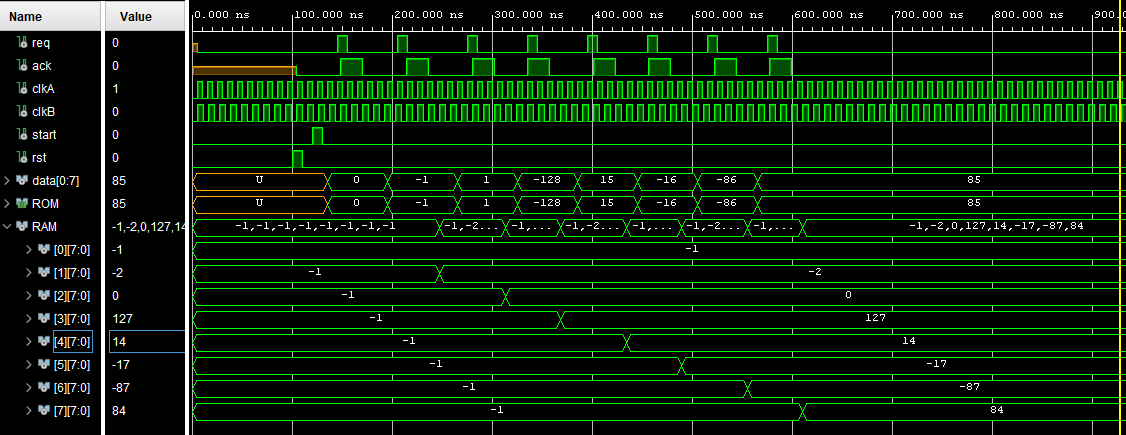
\includegraphics[width=\linewidth]{figure/esercizio8-1/simulazione}
  \caption{Simulazione dell'handshaking}
  \label{fig:esercizio8-1:simulazione}
\end{figure}

Dopo \texttt{start} si osservano otto impulsi di \texttt{req}, ciascuno seguito da un impulso di \texttt{ack} (di durata maggiore, perché \texttt{ack} scende solo dopo che B ha visto \texttt{req} a \texttt{'0'}). Su \texttt{data} compaiono in sequenza i valori della ROM: $0$, $-1$, $1$, $-128$, $15$, $-16$, $-86$, $85$, ossia \texttt{x"00"}, \texttt{x"FF"}, \texttt{x"01"}, \texttt{x"80"}, \texttt{x"0F"}, \texttt{x"F0"}, \texttt{x"AA"}, \texttt{x"55"}. La memoria \texttt{RAM} del nodo B ha inizialmente valore $-1$ (\texttt{x"FF"}) in ogni locazione e viene aggiornata una locazione per volta al termine di ciascun trasferimento. Ad esempio, per la locazione 3 il dato ricevuto è \texttt{x"80"} ($-128$): la somma $\texttt{x"80"} + \texttt{x"FF"}$ dà \texttt{x"7F"} sugli 8 bit, cioè $127$, valore effettivamente letto in \texttt{RAM[3]}. Al termine il contenuto è $-1, -2, 0, 127, 14, -17, -87, 84$.

\begin{risultato}
Le otto somme sono memorizzate nella memoria di B come mostrato in figura, con i due nodi su clock a \SI{10}{ns} e \SI{11}{ns}.
\end{risultato}


\esCapitolo{Processore MIC-1}\label{cap:processore}
\esSezione{Processore MIC-1}\label{sec:esercizio9-1}

\begin{traccia}
A partire dall'implementazione fornita del processore operante secondo il modello IJVM,
\begin{enumerate}[label=\alph*)]
  \item si proceda all'analisi dell'architettura mediante simulazione e si approfondisca lo studio del suo funzionamento per due istruzioni a scelta;
  \item si modifichi un codice operativo a scelta, documentando tutte le modifiche effettuate.
\end{enumerate}
\end{traccia}

% TODO: manca il testbench di simulazione (programma IJVM in memoria, forme d'onda dei registri)



\progetto

Il processore presentato segue l'architettura MIC-1: una parte operativa a \SI{32}{bit}, che contiene i registri e le linee di trasferimento, e un'unità di controllo che, a ogni ciclo di clock, emette un insieme di comandi letti da una memoria ROM di microcodice denominata \texttt{control store}. Il top module \texttt{processor} istanzia le due parti e le collega con quattro gruppi di comandi (ALU, bus C, memoria, bus B), in direzione unità di controllo verso parte operativa, e con tre informazioni di ritorno: il registro \texttt{mbr} e i flag \texttt{n\_flag} e \texttt{z\_flag} dell'ALU.

I componenti del sistema presentato, oltre al package con larghezze dei registi, tipi dei campi di controllo e costanti simboliche per i bit di comando, sono i seguenti:
\begin{enumerate}
  \item \texttt{alu}: unità aritmetico-logica con shifter, ingressi \texttt{a} e \texttt{b}, uscita \texttt{c} e flag \texttt{n} e \texttt{z};
  \item \texttt{control\_store}: memoria di microcodice da 512 parole di \SI{36}{bit};
  \item \texttt{mic1\_cu}: unità di controllo con registro di microistruzione (MIR) e logica di calcolo del prossimo indirizzo;
  \item \texttt{mic1\_datapath}: registri, MBR, multiplexer del bus B e interfaccia verso le memorie;
  \item \texttt{processor}: top module.
\end{enumerate}

I registri hanno ampiezza di \SI{32}{bit} (\texttt{REG\_WIDTH}), tranne \texttt{mbr} che è di \SI{8}{bit} (\texttt{MBR\_WIDTH}) perché contiene un byte d'istruzione. L'indirizzamento della memoria dati passa per \texttt{mar}, il dato per \texttt{mdr}; la memoria istruzioni è indirizzata da \texttt{pc} e fornisce un byte alla volta.

La microistruzione è un vettore di \SI{36}{bit} (\texttt{mir\_type}), suddiviso nei campi seguenti, a partire dal MSB:
\begin{enumerate}
  \item \texttt{Addr} (9 bit): indirizzo della prossima microistruzione;
  \item \texttt{JAM} (3 bit): \texttt{JMPC}, \texttt{JAMN} e \texttt{JAMZ}, segnali utili al controllo del flusso di esecuzione delle microistruzioni;
  \item \texttt{ALU} (8 bit): \texttt{SLL8}, \texttt{SRA1} (segnali per lo shift aritmetico e logico), \texttt{F0}, \texttt{F1} (segnali di selezione della particolare operazione), \texttt{ENA}, \texttt{ENB} (caricamento operandi), \texttt{INVA}, \texttt{INC} (operazioni preliminari sugli operandi);
  \item \texttt{C} (9 bit): un bit di abilitazione per ciascuno dei registri \texttt{H}, \texttt{OPC}, \texttt{TOS}, \texttt{CPP}, \texttt{LV}, \texttt{SP}, \texttt{PC}, \texttt{MDR}, \texttt{MAR}, realizzando di fatto il paradigma orizzontale;
  \item \texttt{Mem} (3 bit): \texttt{WRITE}, \texttt{READ}, \texttt{FETCH} (segnali diretti all'interfaccia di memoria);
  \item \texttt{B} (4 bit): codice del registro da porre sul bus B (paradigma verticale).
\end{enumerate}
% Il codice del campo \texttt{B} seleziona \texttt{mdr} ("0000"), \texttt{pc} ("0001"), \texttt{mbr} con estensione di segno ("0010"), \texttt{mbr} senza segno ("0011"), \texttt{sp} ("0100"), \texttt{lv} ("0101"), \texttt{cpp} ("0110"), \texttt{tos} ("0111") oppure \texttt{opc} ("1000"); con qualunque altro codice, ad esempio "1111", il bus B vale zero.

% \implementazione

% Procediamo in ordine bottom-up. Il package \texttt{common\_defs} definisce i sottotipi dei registri (\texttt{reg\_data\_type} e \texttt{mbr\_data\_type}), i sottotipi dei quattro campi di comando con le posizioni dei singoli bit come costanti \texttt{natural} (ad esempio \texttt{ALU\_INC} o \texttt{C\_SP}), i codici del campo \texttt{B} e i tipi \texttt{mpc\_type} (9 bit) e \texttt{mir\_type} (36 bit).

% \vhdlfile{esercizio9-1/common_defs.vhd}{Package common\_defs}{lst:esercizio9-1:common-defs}

% \paragraph{ALU.}
% L'entità \texttt{alu} ha come ingressi il campo di controllo \texttt{ctrl} (8 bit) e gli operandi \texttt{a} e \texttt{b}, a \SI{32}{bit}, e come uscite il risultato \texttt{c} e i flag \texttt{n} (negativo) e \texttt{z} (zero). L'architettura \texttt{Behavioral} è puramente combinatoria, in stile dataflow. Gli ingressi sono abilitati singolarmente con \texttt{ENA} ed \texttt{ENB}: se il bit vale '0' l'operando è forzato a zero. Il bit \texttt{INVA} complementa l'ingresso \texttt{a}. I bit \texttt{F0} e \texttt{F1} selezionano, tramite un costrutto \texttt{with select}, l'AND ("00"), l'OR ("01"), il complemento di \texttt{b} ("10") oppure la somma \texttt{a + b + inc} ("11"), dove \texttt{inc} è il riporto in ingresso dato dal bit \texttt{INC}. I flag sono calcolati sul risultato prima dello shifter, che infine produce lo scorrimento a sinistra di otto posizioni con \texttt{SLL8} oppure lo scorrimento aritmetico a destra di una posizione con \texttt{SRA1}.

% \vhdlfile{esercizio9-1/alu.vhd}{Implementazione dell'ALU}{lst:esercizio9-1:alu}

% \paragraph{Control store.}
% L'entità \texttt{control\_store} ha un ingresso \texttt{addr} di tipo \texttt{mpc\_type} e un'uscita \texttt{word} di tipo \texttt{mir\_type}. L'architettura \texttt{rom} dichiara una costante di tipo array di 512 microistruzioni; la lettura è asincrona e consiste in un'unica assegnazione concorrente che indicizza l'array con \texttt{addr}. Le posizioni non inizializzate contengono la microistruzione \texttt{NOP}, che non scrive alcun registro, non accede alla memoria e rimanda all'indirizzo 0, cioè al ciclo principale.

% Il microprogramma presente nella memoria è composto da quattro blocchi:
% \begin{enumerate}
%   \item avvio (indirizzi 0x100--0x102): carica in \texttt{mar} il valore di \texttt{sp} avviando una lettura e un fetch, attende un ciclo la memoria e poi copia \texttt{mdr} in \texttt{tos};
%   \item ciclo principale (indirizzo 0x103): incrementa \texttt{pc}, avvia il fetch del byte successivo e salta all'indirizzo ottenuto dall'OR tra il campo \texttt{Addr} (zero) e il contenuto di \texttt{mbr}, ossia al codice operativo letto;
%   \item \texttt{iadd}, opcode 0x65 (indirizzi 0x065--0x067);
%   \item \texttt{halt}, opcode 0xFF (indirizzo 0x0FF): la microistruzione rimanda a se stessa.
% \end{enumerate}
% Poiché il salto \texttt{JMPC} lascia a zero il bit più significativo dell'indirizzo, ogni istruzione ha come indirizzo di partenza il proprio opcode.

% \vhdlfile{esercizio9-1/control_store.vhd}{Implementazione del control store}{lst:esercizio9-1:control-store}

% \paragraph{Unità di controllo.}
% L'entità \texttt{mic1\_cu} riceve \texttt{clk}, \texttt{reset}, il byte \texttt{mbr\_in} e i flag \texttt{n\_flag} e \texttt{z\_flag}, ed emette i quattro gruppi di comando \texttt{alu\_ctrl}, \texttt{c\_ctrl}, \texttt{mem\_ctrl} e \texttt{b\_ctrl}. Un solo process sincrono, \texttt{mir\_proc}, con \texttt{clk} come sensitivity list, aggiorna il registro \texttt{mir} sul fronte di salita: con \texttt{reset} a '1' viene caricata la costante \texttt{RESET\_MIR}, microistruzione senza effetti che rimanda all'indirizzo 0x100 (avvio); altrimenti viene caricata la parola \texttt{cs\_word} letta dal control store. I campi di \texttt{mir} sono resi accessibili tramite \texttt{alias}, ad esempio \texttt{mir\_addr} e \texttt{mir\_jmpc}.

% Il prossimo indirizzo \texttt{mpc} è calcolato in modo combinatorio con la tecnica del bit ORing: gli otto bit bassi sono quelli di \texttt{mir\_addr}, posti in OR con \texttt{mbr\_in} quando \texttt{JMPC} vale '1'; il bit più alto è \texttt{mir\_addr(8)} in OR con \texttt{n\_flag} se \texttt{JAMN} vale '1' e con \texttt{z\_flag} se \texttt{JAMZ} vale '1'. L'indirizzo \texttt{mpc} è collegato a \texttt{control\_store} nell'istanza \texttt{u\_cs}. I comandi verso la parte operativa sono le porzioni di \texttt{mir} assegnate direttamente alle uscite: l'unità di controllo è dunque una macchina di tipo Moore, con comandi dipendenti solo dal registro \texttt{mir}.

% \vhdlfile{esercizio9-1/mic1_cu.vhd}{Implementazione dell'unità di controllo}{lst:esercizio9-1:mic1-cu}

% \paragraph{Parte operativa.}
% L'entità \texttt{mic1\_datapath} riceve i comandi dall'unità di controllo e le uscite della memoria, ed espone \texttt{mbr\_out}, \texttt{n\_flag} e \texttt{z\_flag}; verso le memorie esporta \texttt{mem\_data\_addr}, \texttt{mem\_data\_out}, \texttt{mem\_data\_we} e \texttt{mem\_instr\_addr}. L'architettura \texttt{rtl} dichiara i registri \texttt{mar}, \texttt{mdr}, \texttt{pc}, \texttt{sp}, \texttt{lv}, \texttt{cpp}, \texttt{tos}, \texttt{opc}, \texttt{h} e \texttt{mbr}, più tre flip-flop di appoggio \texttt{rd\_ff}, \texttt{wr\_ff} e \texttt{fetch\_ff}.

% Il process \texttt{reg\_proc}, sincrono su \texttt{clk}, gestisce tutti i registri. Il reset sincrono azzera i registri e inizializza \texttt{sp} a \texttt{x"00000101"}, \texttt{lv} a \texttt{x"00000100"} e \texttt{cpp} a \texttt{x"00000080"}. Nel funzionamento normale ogni registro è caricato dal bus \texttt{c\_bus} quando il rispettivo bit del campo \texttt{c\_ctrl} vale '1'. Il registro \texttt{mdr} ha una doppia sorgente: il bus C, che ha la precedenza, oppure \texttt{mem\_data\_in} quando \texttt{rd\_ff} vale '1'. Il registro \texttt{mbr} si carica da \texttt{mem\_instr\_in} quando \texttt{fetch\_ff} vale '1'. Le richieste di lettura, scrittura e fetch emesse da una microistruzione sono memorizzate in \texttt{rd\_ff}, \texttt{wr\_ff} e \texttt{fetch\_ff} e producono effetto nel ciclo successivo; \texttt{wr\_ff} pilota direttamente \texttt{mem\_data\_we}. Per questo, dopo una microistruzione con \texttt{READ} il dato non è ancora in \texttt{mdr}, e la microistruzione seguente non può ancora usarlo.

% Il bus B è descritto con un costrutto \texttt{with select} su \texttt{b\_ctrl}. Il byte \texttt{mbr} è esteso a \SI{32}{bit} in due modi, con segno (\texttt{mbr\_s}) e senza segno (\texttt{mbr\_u}), tramite \texttt{resize} su tipi \texttt{signed} e \texttt{unsigned}. Le uscite \texttt{mem\_data\_addr}, \texttt{mem\_data\_out} e \texttt{mem\_instr\_addr} sono collegate ai registri \texttt{mar}, \texttt{mdr} e \texttt{pc}.

% \vhdlfile{esercizio9-1/mic1_datapath.vhd}{Implementazione della parte operativa}{lst:esercizio9-1:mic1-datapath}

% \paragraph{Top module.}
% Il top module è l'entità \texttt{processor}, contenuta nel file \texttt{mic1.vhd}, con architettura \texttt{structural}. Le porte sono \texttt{clk} e \texttt{reset}, l'interfaccia dati (\texttt{mem\_data\_addr}, \texttt{mem\_data\_out}, \texttt{mem\_data\_in}, \texttt{mem\_data\_we}) e l'interfaccia istruzioni (\texttt{mem\_instr\_addr}, \texttt{mem\_instr\_in}). I segnali interni \texttt{alu\_ctrl}, \texttt{c\_ctrl}, \texttt{mem\_ctrl}, \texttt{b\_ctrl}, \texttt{mbr}, \texttt{n\_flag} e \texttt{z\_flag} collegano, tramite port mapping per nome, le istanze \texttt{u\_dp} (\texttt{mic1\_datapath}) e \texttt{u\_cu} (\texttt{mic1\_cu}).

% \vhdlfile{esercizio9-1/mic1.vhd}{Implementazione del top module}{lst:esercizio9-1:mic1}

% \paragraph{Microprogramma: avvio e istruzione \texttt{iadd}.}


\subsubsection{Analisi istruzioni}
Visioniamo come sono codificate nel control store due sequenze. La prima è l'avvio, a partire dall'indirizzo 0x100 raggiunto dopo il reset:
\begin{enumerate}
  \item \texttt{MAR = SP; rd; fetch} $\rightarrow$ i campi attivi sono \texttt{ENB}, \texttt{F1} e \texttt{B = SP}; poiché \texttt{ENA} è a '0', l'ALU lascia passare il solo bus B (\texttt{F0F1} = "01", OR con zero). Il risultato è scritto in \texttt{mar} e sono richieste una lettura e un fetch;
  \item attesa della memoria, con una microistruzione che non comanda alcun registro;
  \item \texttt{TOS = MDR} $\rightarrow$ il valore letto è copiato in \texttt{tos} con la stessa configurazione dell'ALU e \texttt{B = MDR}.
\end{enumerate}
Segue la microistruzione del ciclo principale in 0x103, \texttt{PC = PC + 1; fetch; goto (MBR)} $\rightarrow$ con \texttt{ENA} a '0', \texttt{ENB} e \texttt{INC} a '1' e \texttt{F0F1} = "11" l'ALU calcola \texttt{pc + 1}; il risultato è scritto in \texttt{pc}, viene richiesto un nuovo fetch e il bit \texttt{JMPC} manda il controllo all'indirizzo contenuto in \texttt{mbr}.

L'istruzione \texttt{iadd}, con opcode 0x65, estrae due interi dallo stack, ne calcola la somma e la riporta in cima. È composta da tre microistruzioni:
\begin{enumerate}
  \item \texttt{MAR = SP = SP - 1; rd} $\rightarrow$ con \texttt{ENA} a '0' e \texttt{INVA} a '1' il primo operando dell'ALU è \texttt{x"FFFFFFFF"} (-1, complemento di x00000000), e la somma con \texttt{sp} (\texttt{B = SP}) dà \texttt{sp - 1}; il risultato è scritto sia in \texttt{sp} sia in \texttt{mar} e parte la lettura del secondo operando;
  \item \texttt{H = TOS} $\rightarrow$ il registro \texttt{tos}, posto sul bus B, è copiato in \texttt{h}, mentre la lettura è in corso;
  \item \texttt{MDR = TOS = MDR + H; wr; goto main}: con \texttt{ENA}, \texttt{ENB} e \texttt{F0F1} = "11" l'ALU somma \texttt{h} e \texttt{mdr} (\texttt{B = MDR}); il risultato è scritto in \texttt{mdr} e in \texttt{tos}, viene richiesta la scrittura in memoria e il campo \texttt{Addr} rimanda all'indirizzo 0x103, da cui parte l'istruzione successiva.
\end{enumerate}

\subsubsection{Sintesi istruzioni}
In questa sezione presentiamo la modifica dell'istruzione \texttt{DUP} (x59). L'istruzione originale copia la parola in cima allo stack e la \textit{spinge} sullo stack stack. L'idea è quella di implementare \texttt{TRIP} (x59), ovvero la copia della parola in cima allo stack per due volte. 

\vhdlfile{esercizio9-1/dup.vhdl}{Istruzione DUP}{lst:esercizio9-1:dup}

\noindent
L'istruzione \texttt{dup} è composta da due microistruzioni:

\begin{enumerate}
  \item MAR = SP = SP + 1; $\rightarrow$ l'istruzione comanda la ALU con \texttt{F0 F1 = 11}, \texttt{ENA = 0}, \texttt{ENB = 1}, \texttt{INVA = 0}, \texttt{INC = 1} → \texttt{0 + SP + 1}, ovvero somma l'ingresso B con 0 e 1.Il risultato è scritto sia in \texttt{SP} che in \texttt{MAR};
  \item richiediamo una scrittura all'indirizzo aggiornato di \texttt{MAR} con il vecchio valore di \texttt{TOS}, ovvero il valore da duplicare. 
\end{enumerate}

La modifica consiste nell'aggiornamento dello stack pointere del memory address register; Il top of stack già conteneva il valore da duplicare, quindi richiediamo una scrittura del vecchio \texttt{TOS} all'indirizzo aggiornato di \texttt{MAR} sovrascrivendo \texttt{MDR}, e infine richiediamo la stessa operazione di scrittura (i registri di indirizzo e dato sono già impostati) incrementando nuovamente lo \texttt{SP} e il \texttt{MAR}. Infine si salta alla microistruzione principale \texttt{main}.

\vhdlfile{esercizio9-1/trip.vhdl}{Istruzione TRIP}{lst:esercizio9-1:trip}
\vhdlfile{esercizio9-1/program.ajvm}{Modifica al programma}{lst:esercizio9-1:program}
\vhdlfile{esercizio9-1/processor_tb.vhdl}{Modifica al testbench}{lst:esercizio9-1:tb}

\vhdlfile{esercizio9-1/bash_history.vhdl}{.bash\_history}{lst:esercizio9-1:shell}




\esCapitolo{Interfaccia seriale}\label{cap:interfaccia-seriale}
\esercizioDaSvolgere{Comunicazione seriale UART-RS232}{esercizio10-1}


\esCapitolo{Switch multistadio}\label{cap:switch-multistadio}
\esSezione{Switch multistadio omega network}\label{sec:esercizio11-1}

\begin{traccia}
Progettare ed implementare in VHDL uno switch multistadio secondo il modello omega network. Lo switch deve consentire lo scambio di messaggi di 2 bit ciascuno da un nodo sorgente a un nodo destinazione in una rete con 4 nodi, implementando uno schema a priorità fissa fra i nodi (es. nodo 1 più prioritario, con priorità decrescenti fino al nodo 4).
\end{traccia}

\progetto

La omega network è una rete di interconnessione multistadio: una rete $N \times N$ è formata da $\log_2 N$ stadi, ciascuno composto da $N/2$ switch elementari $2 \times 2$, collegati tra loro con lo schema detto \emph{perfect shuffling}. Lo schema richiama la mescolata di un mazzo di carte: il mazzo viene diviso in due metà e le carte vengono intercalate una per una, così che a ogni coppia di posizioni adiacenti corrisponda una carta della metà alta e una della metà bassa. Applicato ai collegamenti, ogni switch riceve un ingresso dalla prima metà dei nodi e uno dalla seconda; lo stesso criterio vale tra uno stadio e il successivo, dove la prima uscita di ciascuno switch va al primo switch dello stadio seguente e la seconda uscita al secondo.

Con $N=4$ gli stadi sono $\log_2 4 = 2$, per un totale di quattro switch. I nodi sono numerati da 1 a 4 e identificati dai codici $00_2$, $01_2$, $10_2$, $11_2$. Gli ingressi sono accoppiati come $(x1, x3)$ e $(x2, x4)$ sul primo stadio, e le uscite dei due switch del primo stadio sono distribuite sul secondo secondo lo schema appena descritto. La topologia così realizzata è visibile in figura~\ref{fig:esercizio11-1:topologia}.

\begin{figure}[htbp]
  \centering
  \resizebox{0.95\linewidth}{!}{%
  \begin{tikzpicture}[font=\sffamily\small]
    % ---------------- stadio 1 ----------------
    \node[font=\sffamily\bfseries\small] at (3,4.95) {Stadio 1};
    \node[font=\footnotesize] at (3,4.5) {\texttt{s\_src(1)}, \texttt{s\_dst(1)}};
    \node[blocco, minimum width=2.2cm, minimum height=1.6cm] (o1) at (3,3) {};
    \node[font=\footnotesize] at (3,3) {\texttt{omega1}};
    \node[font=\scriptsize, anchor=west] at (1.95,3.4) {\texttt{x0}};
    \node[font=\scriptsize, anchor=west] at (1.95,2.6) {\texttt{x1}};
    \node[font=\scriptsize, anchor=east] at (4.05,3.4) {\texttt{y0}};
    \node[font=\scriptsize, anchor=east] at (4.05,2.6) {\texttt{y1}};

    \node[blocco, minimum width=2.2cm, minimum height=1.6cm] (o2) at (3,0) {};
    \node[font=\footnotesize] at (3,0) {\texttt{omega2}};
    \node[font=\scriptsize, anchor=west] at (1.95,0.4) {\texttt{x0}};
    \node[font=\scriptsize, anchor=west] at (1.95,-0.4) {\texttt{x1}};
    \node[font=\scriptsize, anchor=east] at (4.05,0.4) {\texttt{y0}};
    \node[font=\scriptsize, anchor=east] at (4.05,-0.4) {\texttt{y1}};

    % ---------------- stadio 2 ----------------
    \node[font=\sffamily\bfseries\small] at (10,4.95) {Stadio 2};
    \node[font=\footnotesize] at (10,4.5) {\texttt{s\_src(0)}, \texttt{s\_dst(0)}};
    \node[blocco, minimum width=2.2cm, minimum height=1.6cm] (o3) at (10,3) {};
    \node[font=\footnotesize] at (10,3) {\texttt{omega3}};
    \node[font=\scriptsize, anchor=west] at (8.95,3.4) {\texttt{x0}};
    \node[font=\scriptsize, anchor=west] at (8.95,2.6) {\texttt{x1}};
    \node[font=\scriptsize, anchor=east] at (11.05,3.4) {\texttt{y0}};
    \node[font=\scriptsize, anchor=east] at (11.05,2.6) {\texttt{y1}};

    \node[blocco, minimum width=2.2cm, minimum height=1.6cm] (o4) at (10,0) {};
    \node[font=\footnotesize] at (10,0) {\texttt{omega4}};
    \node[font=\scriptsize, anchor=west] at (8.95,0.4) {\texttt{x0}};
    \node[font=\scriptsize, anchor=west] at (8.95,-0.4) {\texttt{x1}};
    \node[font=\scriptsize, anchor=east] at (11.05,0.4) {\texttt{y0}};
    \node[font=\scriptsize, anchor=east] at (11.05,-0.4) {\texttt{y1}};

    % ---------------- ingressi ----------------
    \draw[bus] (-0.3,3.4) -- node[larghezza=2, pos=0.55]{/} (1.9,3.4);
    \node[anchor=east] at (-0.3,3.4) {\texttt{x1}};
    \draw[bus] (-0.3,2.6) -- node[larghezza=2, pos=0.55]{/} (1.9,2.6);
    \node[anchor=east] at (-0.3,2.6) {\texttt{x3}};
    \draw[bus] (-0.3,0.4) -- node[larghezza=2, pos=0.55]{/} (1.9,0.4);
    \node[anchor=east] at (-0.3,0.4) {\texttt{x2}};
    \draw[bus] (-0.3,-0.4) -- node[larghezza=2, pos=0.55]{/} (1.9,-0.4);
    \node[anchor=east] at (-0.3,-0.4) {\texttt{x4}};

    % ---------------- collegamenti perfect shuffle ----------------
    % l1: omega1.y0 -> omega3.x0
    \draw[bus] (4.1,3.4) -- (8.9,3.4);
    \node[font=\footnotesize, above] at (4.65,3.4) {\texttt{l1}};
    \node[larghezza=2] at (7.8,3.4) {/};
    % l2: omega1.y1 -> omega4.x0
    \draw[bus] (4.1,2.6) -- (5.3,2.6) -- (7.7,0.4) -- (8.9,0.4);
    \node[font=\footnotesize, below] at (4.7,2.6) {\texttt{l2}};
    \node[larghezza=2] at (8.3,0.4) {/};
    % l3: omega2.y0 -> omega3.x1
    \draw[bus] (4.1,0.4) -- (5.3,0.4) -- (7.7,2.6) -- (8.9,2.6);
    \node[font=\footnotesize, below] at (4.7,0.4) {\texttt{l3}};
    \node[larghezza=2] at (8.3,2.6) {/};
    % l4: omega2.y1 -> omega4.x1
    \draw[bus] (4.1,-0.4) -- (8.9,-0.4);
    \node[font=\footnotesize, below] at (4.65,-0.4) {\texttt{l4}};
    \node[larghezza=2] at (7.8,-0.4) {/};

    % ---------------- uscite ----------------
    \draw[bus] (11.1,3.4) -- node[larghezza=2, pos=0.4]{/} (13.4,3.4);
    \node[anchor=west] at (13.4,3.4) {\texttt{y1}};
    \draw[bus] (11.1,2.6) -- node[larghezza=2, pos=0.4]{/} (13.4,2.6);
    \node[anchor=west] at (13.4,2.6) {\texttt{y2}};
    \draw[bus] (11.1,0.4) -- node[larghezza=2, pos=0.4]{/} (13.4,0.4);
    \node[anchor=west] at (13.4,0.4) {\texttt{y3}};
    \draw[bus] (11.1,-0.4) -- node[larghezza=2, pos=0.4]{/} (13.4,-0.4);
    \node[anchor=west] at (13.4,-0.4) {\texttt{y4}};
  \end{tikzpicture}}
  \caption{Topologia della omega network a 4 nodi}
  \label{fig:esercizio11-1:topologia}
\end{figure}

L'instradamento sfrutta l'indirizzo del nodo destinazione: ogni stadio esamina un bit, a partire dal più significativo, e indirizza il messaggio sull'uscita alta dello switch se il bit vale \texttt{'0'}, su quella bassa se vale \texttt{'1'}. Si consideri, ad esempio, il trasferimento dal nodo 3 ($10_2$) al nodo 2 ($01_2$). Nel primo stadio il nodo 3 entra dall'ingresso \texttt{x1} di \texttt{omega1}, e il bit più significativo della destinazione, $0$, porta il messaggio su \texttt{y0}, ossia sul collegamento \texttt{l1}. Nel secondo stadio il bit meno significativo, $1$, lo indirizza sull'uscita \texttt{y1} di \texttt{omega3}, che coincide con \texttt{y2}, l'uscita del nodo 2.

Il sistema completo si compone di due parti, riportate in figura~\ref{fig:esercizio11-1:architettura}: la rete di switch, descritta dall'entità \texttt{omega\_network\_4}, e un componente di arbitraggio, \texttt{arbitro}, che realizza la priorità fissa. L'\texttt{arbitro} riceve il vettore di richieste \texttt{req} a 4 bit, in cui \texttt{req(0)} appartiene al nodo 1, il più prioritario, e \texttt{req(3)} al nodo 4; produce il segnale \texttt{src\_out}, a 2 bit, con il codice del nodo ammesso a trasmettere, che pilota l'ingresso \texttt{s\_src} della rete. Il codice del nodo destinazione è invece fornito dall'esterno attraverso \texttt{s\_dst}. I messaggi di 2 bit viaggiano sui bus \texttt{x1}\ldots\texttt{x4} in ingresso e \texttt{y1}\ldots\texttt{y4} in uscita.

\begin{figure}[htbp]
  \centering
  \resizebox{0.9\linewidth}{!}{%
  \begin{tikzpicture}[font=\sffamily\small]
    \node[ctrl, minimum width=3.6cm] (arb) at (2.7,4.6) {\texttt{arbitro}\\[-1pt]{\footnotesize priorità a \texttt{req(0)}}};
    \node[blocco, minimum width=4.4cm, minimum height=4.4cm] (om) at (8,0) {\texttt{omega\_network\_4}\\[-1pt]{\footnotesize 4 switch su 2 stadi}};

    % richieste
    \draw[bus] (-0.5,4.6) -- node[larghezza=4, pos=0.55]{/} (arb.west);
    \node[anchor=east] at (-0.5,4.6) {\texttt{req}};
    % src_out -> s_src
    \draw[bus] (arb.east) -- node[larghezza=2, pos=0.57]{/} (8,4.6) -- (8,2.2);
    \node[font=\footnotesize, above] at (5.3,4.6) {\texttt{src\_out}};
    \node[font=\footnotesize, above] at (7.4,4.6) {\texttt{s\_src}};

    % ingressi dati
    \draw[bus] (0.0,1.5) -- node[larghezza=2, pos=0.5]{/} (5.8,1.5);
    \node[anchor=east] at (0.0,1.5) {\texttt{x1}};
    \draw[bus] (0.0,0.5) -- node[larghezza=2, pos=0.5]{/} (5.8,0.5);
    \node[anchor=east] at (0.0,0.5) {\texttt{x2}};
    \draw[bus] (0.0,-0.5) -- node[larghezza=2, pos=0.5]{/} (5.8,-0.5);
    \node[anchor=east] at (0.0,-0.5) {\texttt{x3}};
    \draw[bus] (0.0,-1.5) -- node[larghezza=2, pos=0.5]{/} (5.8,-1.5);
    \node[anchor=east] at (0.0,-1.5) {\texttt{x4}};

    % uscite dati
    \draw[bus] (10.2,1.5) -- node[larghezza=2, pos=0.5]{/} (13.6,1.5);
    \node[anchor=west] at (13.6,1.5) {\texttt{y1}};
    \draw[bus] (10.2,0.5) -- node[larghezza=2, pos=0.5]{/} (13.6,0.5);
    \node[anchor=west] at (13.6,0.5) {\texttt{y2}};
    \draw[bus] (10.2,-0.5) -- node[larghezza=2, pos=0.5]{/} (13.6,-0.5);
    \node[anchor=west] at (13.6,-0.5) {\texttt{y3}};
    \draw[bus] (10.2,-1.5) -- node[larghezza=2, pos=0.5]{/} (13.6,-1.5);
    \node[anchor=west] at (13.6,-1.5) {\texttt{y4}};

    % destinazione
    \draw[bus] (0.0,-3.4) -- node[larghezza=2, pos=0.55]{/} (8,-3.4) -- (8,-2.2);
    \node[anchor=east] at (0.0,-3.4) {\texttt{s\_dst}};
  \end{tikzpicture}}
  \caption{Architettura del sistema}
  \label{fig:esercizio11-1:architettura}
\end{figure}

\implementazione

Si procede in modo bottom-up, partendo dai due componenti che compongono lo switch elementare. Il multiplexer \texttt{mux2\_1} ha due ingressi dati a 2 bit, \texttt{x0} e \texttt{x1}, la selezione \texttt{s} a 1 bit e l'uscita \texttt{z} a 2 bit. L'architettura è dataflow e si basa su un costrutto \texttt{with select}: con \texttt{s} pari a \texttt{'0'} l'uscita è \texttt{x0}, in ogni altro caso \texttt{x1}.

\vhdlfile{esercizio11-1/mux2_1.vhd}{Implementazione MUX 2:1}{lst:esercizio11-1:mux2-1}

Il demultiplexer \texttt{demux1\_2} riceve il dato \texttt{z} a 2 bit e la selezione \texttt{s}, e dispone di due uscite a 2 bit, \texttt{y0} e \texttt{y1}. Anche questa architettura è dataflow, con due assegnamenti condizionati: l'uscita indicata da \texttt{s} riceve \texttt{z}, mentre l'altra viene forzata a \texttt{"00"}. Un messaggio non destinato a una certa uscita lascia quindi su di essa il valore nullo.

\vhdlfile{esercizio11-1/demux1_2.vhd}{Implementazione DEMUX 1:2}{lst:esercizio11-1:demux1-2}

Lo switch elementare \texttt{switch2\_2} mette in serie un \texttt{mux2\_1} e un \texttt{demux1\_2}, secondo la struttura illustrata in figura~\ref{fig:esercizio11-1:switch}. Gli ingressi sono \texttt{x0} e \texttt{x1}, le uscite \texttt{y0} e \texttt{y1}, tutti a 2 bit, e la selezione \texttt{s} è un vettore a 2 bit: \texttt{s(0)} comanda il multiplexer, che sceglie quale ingresso trasmettere, mentre \texttt{s(1)} comanda il demultiplexer, che sceglie su quale uscita inviarlo. Il segnale interno \texttt{z} collega l'uscita del primo componente all'ingresso del secondo.

\begin{figure}[htbp]
  \centering
  \resizebox{0.9\linewidth}{!}{%
  \begin{tikzpicture}[font=\sffamily\small]
    \draw[dashed, thick] (0.6,-3.5) rectangle (11.4,2.3);
    \node[anchor=north west, font=\sffamily\footnotesize\bfseries] at (0.7,2.25) {\texttt{switch2\_2}};

    \node[blocco, minimum width=2.6cm, minimum height=2.0cm] (mx) at (3.4,0) {\texttt{mux2\_1}\\[-1pt]{\footnotesize istanza \texttt{mux}}};
    \node[blocco, minimum width=2.6cm, minimum height=2.0cm] (dm) at (9.4,0) {\texttt{demux1\_2}\\[-1pt]{\footnotesize istanza \texttt{demux}}};

    % ingressi
    \draw[bus] (-1.2,0.5) -- node[larghezza=2, pos=0.3]{/} (2.1,0.5);
    \node[anchor=east] at (-1.2,0.5) {\texttt{x0}};
    \draw[bus] (-1.2,-0.5) -- node[larghezza=2, pos=0.3]{/} (2.1,-0.5);
    \node[anchor=east] at (-1.2,-0.5) {\texttt{x1}};

    % z
    \draw[bus] (4.7,0) -- (8.1,0);
    \node[font=\footnotesize, above] at (5.3,0) {\texttt{z}};
    \node[larghezza=2] at (7.4,0) {/};

    % uscite
    \draw[bus] (10.7,0.5) -- node[larghezza=2, pos=0.8]{/} (13.2,0.5);
    \node[anchor=west] at (13.2,0.5) {\texttt{y0}};
    \draw[bus] (10.7,-0.5) -- node[larghezza=2, pos=0.8]{/} (13.2,-0.5);
    \node[anchor=west] at (13.2,-0.5) {\texttt{y1}};

    % selezione
    \draw[very thick] (-1.2,-2.8) -- (9.4,-2.8);
    \node[larghezza=2] at (0.2,-2.8) {/};
    \node[anchor=east] at (-1.2,-2.8) {\texttt{s}};
    \fill (3.4,-2.8) circle (1.5pt);
    \draw[seg] (3.4,-2.8) -- (3.4,-1.0);
    \node[font=\footnotesize, anchor=west] at (3.5,-1.9) {\texttt{s(0)}};
    \draw[seg] (9.4,-2.8) -- (9.4,-1.0);
    \node[font=\footnotesize, anchor=west] at (9.5,-1.9) {\texttt{s(1)}};
  \end{tikzpicture}}
  \caption{Struttura dello switch elementare}
  \label{fig:esercizio11-1:switch}
\end{figure}

L'architettura \texttt{structural} non dichiara componenti: le due istanze, \texttt{mux} e \texttt{demux}, sono create istanziando direttamente le entità, ossia \texttt{work.mux2\_1} e \texttt{work.demux1\_2} nella loro architettura dataflow, e collegate tramite port mapping.

\vhdlfile{esercizio11-1/switch2_2.vhd}{Implementazione dello switch 2x2}{lst:esercizio11-1:switch2-2}

Il componente \texttt{arbitro} implementa la priorità fissa tra i nodi. L'ingresso \texttt{req} è un vettore a 4 bit con una richiesta di trasmissione per nodo, mentre l'uscita \texttt{src\_out} è il codice a 2 bit del nodo scelto. L'architettura dataflow usa un assegnamento condizionato che esamina i bit di \texttt{req} in ordine: \texttt{"00"} se \texttt{req(0)} è alto, \texttt{"01"} se lo è \texttt{req(1)}, \texttt{"10"} per \texttt{req(2)}, \texttt{"11"} in tutti gli altri casi. Il nodo 1 prevale quindi su tutti gli altri e il nodo 4 viene selezionato solo in assenza di richieste dai nodi precedenti.

\vhdlfile{esercizio11-1/arbitro.vhd}{Implementazione dell'arbitro}{lst:esercizio11-1:arbitro}

Definiti i componenti, il top module \texttt{omega\_network\_4} li compone con un approccio strutturale, come mostrato in figura~\ref{fig:esercizio11-1:topologia}. Le porte sono i quattro ingressi \texttt{x1}\ldots\texttt{x4}, le quattro uscite \texttt{y1}\ldots\texttt{y4}, tutti a 2 bit, e i due codici di selezione \texttt{s\_src} e \texttt{s\_dst}, a 2 bit ciascuno. I segnali interni \texttt{l1}\ldots\texttt{l4} sono i collegamenti tra i due stadi. Il primo stadio è formato da \texttt{omega1}, che riceve \texttt{x1} e \texttt{x3} e produce \texttt{l1} e \texttt{l2}, e da \texttt{omega2}, che riceve \texttt{x2} e \texttt{x4} e produce \texttt{l3} e \texttt{l4}. Il secondo stadio è formato da \texttt{omega3}, con ingressi \texttt{l1} e \texttt{l3} e uscite \texttt{y1} e \texttt{y2}, e da \texttt{omega4}, con ingressi \texttt{l2} e \texttt{l4} e uscite \texttt{y3} e \texttt{y4}. Ogni stadio usa un solo bit di ciascun codice: i due switch del primo stadio ricevono \texttt{s\_src(1)} come selezione del multiplexer e \texttt{s\_dst(1)} come selezione del demultiplexer, mentre quelli del secondo stadio usano \texttt{s\_src(0)} e \texttt{s\_dst(0)}.

\vhdlfile{esercizio11-1/omega_network_4.vhd}{Implementazione dell'omega network a 4 nodi}{lst:esercizio11-1:omega-network-4}

\begin{osservazione}
Nei file sorgente l'\texttt{arbitro} e la rete \texttt{omega\_network\_4} sono componenti separati: \texttt{src\_out} va collegato a \texttt{s\_src} a un livello gerarchico superiore, mentre nel testbench seguente \texttt{s\_src} è pilotato direttamente. In assenza di richieste l'\texttt{arbitro} restituisce lo stesso codice \texttt{"11"} del nodo 4.
\end{osservazione}

\simulazione

Il testbench \texttt{omega\_network\_4\_tb} ha un'entità senza porte e dichiara i segnali \texttt{x1}\ldots\texttt{x4}, \texttt{y1}\ldots\texttt{y4}, \texttt{s\_src} e \texttt{s\_dst}. La rete è istanziata come \texttt{dut} e un unico process, \texttt{stim}, assegna ai quattro ingressi dati costanti: \texttt{x1} $=$ \texttt{"01"}, \texttt{x2} $=$ \texttt{"11"}, \texttt{x3} $=$ \texttt{"10"}, \texttt{x4} $=$ \texttt{"01"}. Si provano poi quattro trasferimenti, ciascuno mantenuto per \SI{10}{\nano\second}:

\begin{enumerate}
  \item nodo 1 verso nodo 4 (\texttt{s\_src} $=$ \texttt{"00"}, \texttt{s\_dst} $=$ \texttt{"11"}): ci si aspetta \texttt{y4} $=$ \texttt{"01"} e \texttt{y1} $=$ \texttt{"00"};
  \item nodo 3 verso nodo 2 (\texttt{"10"}, \texttt{"01"}): ci si aspetta \texttt{y2} $=$ \texttt{"10"};
  \item nodo 2 verso nodo 3 (\texttt{"01"}, \texttt{"10"}): ci si aspetta \texttt{y3} $=$ \texttt{"11"};
  \item nodo 4 verso nodo 1 (\texttt{"11"}, \texttt{"00"}): ci si aspetta \texttt{y1} $=$ \texttt{"01"}.
\end{enumerate}

Le attese sono verificate con \texttt{assert}, con severità \texttt{error}; il process termina con un \texttt{report} di fine test e con \texttt{wait}.

\vhdlfile{esercizio11-1/omega_network_4_tb.vhd}{Testbench dell'omega network a 4 nodi}{lst:esercizio11-1:omega-network-4-tb}

Il risultato della simulazione è riportato in figura~\ref{fig:esercizio11-1:simulazione}.

\begin{figure}[htbp]
  \centering
  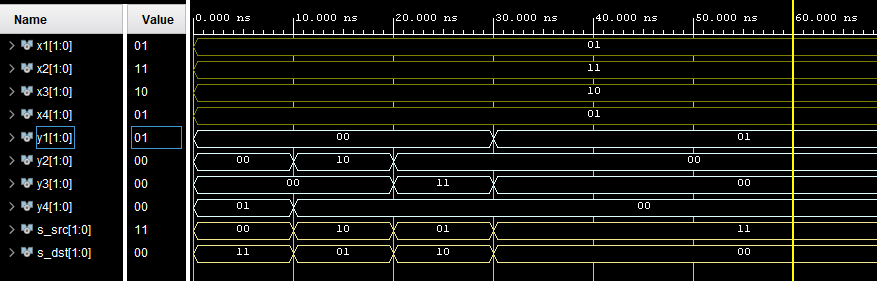
\includegraphics[width=0.95\linewidth]{figure/esercizio11-1/simulazione}
  \caption{Simulazione della omega network a 4 nodi}
  \label{fig:esercizio11-1:simulazione}
\end{figure}

Gli ingressi restano costanti per tutta la durata, mentre \texttt{s\_src} e \texttt{s\_dst} cambiano ogni \SI{10}{\nano\second}. Si legga il secondo intervallo, da \SI{10}{\nano\second} a \SI{20}{\nano\second}: \texttt{s\_src} vale \texttt{"10"} e \texttt{s\_dst} vale \texttt{"01"}, ossia il nodo 3 trasmette al nodo 2. Il dato di \texttt{x3}, \texttt{"10"}, compare su \texttt{y2}, mentre \texttt{y1}, \texttt{y3} e \texttt{y4} restano a \texttt{"00"}. Nello stesso modo, nel primo intervallo \texttt{y4} vale \texttt{"01"}, il valore di \texttt{x1}; nel terzo \texttt{y3} vale \texttt{"11"}, il valore di \texttt{x2}; dal quarto in poi \texttt{y1} vale \texttt{"01"}, il valore di \texttt{x4}.

\begin{risultato}
I quattro trasferimenti producono \texttt{y4} $=$ \texttt{"01"}, \texttt{y2} $=$ \texttt{"10"}, \texttt{y3} $=$ \texttt{"11"} e \texttt{y1} $=$ \texttt{"01"}, e tutte le altre uscite restano a \texttt{"00"}.
\end{risultato}


\esCapitolo{Prova d'esame}\label{cap:prova-esame}
\esercizioDaSvolgere{Prova d'esame di dicembre 2024}{esercizio12-1}


%% === CONTENUTO ELABORATO ===

% ----------------------------------------------------------------------------------------
% APPENDICE: componenti elementari riusati in più esercizi
% ----------------------------------------------------------------------------------------
\appendix

\end{document}
